
%% abtex2-modelo-trabalho-academico.tex, v-1.9 laurocesar
%% Copyright 2012-2013 by abnTeX2 group at http://abntex2.googlecode.com/ 
%%
%% This work may be distributed and/or modified under the
%% conditions of the LaTeX Project Public License, either version 1.3
%% of this license or (at your option) any later version.
%% The latest version of this license is in
%%   http://www.latex-project.org/lppl.txt
%% and version 1.3 or later is part of all distributions of LaTeX
%% version 2005/12/01 or later.
%%
%% This work has the LPPL maintenance status `maintained'.
%% 
%% The Current Maintainer of this work is the abnTeX2 team, led
%% by Lauro César Araujo. Further information are available on 
%% http://abntex2.googlecode.com/
%%
%% This work consists of the files abntex2-modelo-trabalho-academico.tex,
%% abntex2-modelo-include-comandos and abntex2-modelo-references.bib
%%

% ------------------------------------------------------------------------
% ------------------------------------------------------------------------
% abnTeX2: Modelo de Trabalho Academico (tese de doutorado, dissertacao de
% mestrado e trabalhos monograficos em geral) em conformidade com 
% ABNT NBR 14724:2011: Informacao e documentacao - Trabalhos academicos -
% Apresentacao
% ------------------------------------------------------------------------
% ------------------------------------------------------------------------

\documentclass[
	% -- opções da classe memoir --
	12pt,				% tamanho da fonte
	openany,			% capítulos começam em pág ímpar (insere página vazia caso preciso) - openright ou openany
	oneside,			% para impressão em verso e anverso. Oposto a oneside
	a4paper,			% tamanho do papel. 
	% -- opções da classe abntex2 --
	%chapter=TITLE,		% títulos de capítulos convertidos em letras maiúsculas
	%section=TITLE,		% títulos de seções convertidos em letras maiúsculas
	%subsection=TITLE,	% títulos de subseções convertidos em letras maiúsculas
	%subsubsection=TITLE,% títulos de subsubseções convertidos em letras maiúsculas
	% -- opções do pacote babel --
	english,			% idioma adicional para hifenização
	french,				% idioma adicional para hifenização
	spanish,			% idioma adicional para hifenização
	brazil				% o último idioma é o principal do documento
	]{abntex2}

% ---
% PACOTES
% ---

% ---
% Pacotes fundamentais 
% ---
\usepackage{lmodern}			% Usa a fonte Latin Modern			
\usepackage[T1]{fontenc}		% Selecao de codigos de fonte.
\usepackage[utf8]{inputenc}		% Codificacao do documento (conversão automática dos acentos)
\usepackage{lastpage}			% Usado pela Ficha catalográfica
\usepackage{indentfirst}		% Indenta o primeiro parágrafo de cada seção.
\usepackage{color}				% Controle das cores
\usepackage{graphicx}			% Inclusão de gráficos
\usepackage[export]{adjustbox}  % Permite usar a opção frame ou fbox, para criar margem nas figuras
\usepackage[singlelinecheck=false]{caption} % Manter caption à esquerda
\usepackage{microtype} 			% para melhorias de justificação
\usepackage{rotating}           %rotação de texto
%\usepackage[landscape]{geometry}% http://ctan.org/pkg/geometry
\usepackage{array}              % http://ctan.org/pkg/array
\usepackage[table,xcdraw]{xcolor}
\usepackage[printonlyused]{acronimos-extendido}
\usepackage{textcase}
\usepackage{caption}
\usepackage{subcaption}
\usepackage{multirow}
\usepackage{booktabs}
\usepackage{makecell}
\usepackage{pifont}
\usepackage{longtable}
\usepackage{setspace}
\usepackage{ltablex}
\usepackage[T1]{fontenc}
\usepackage{tgbonum}
\usepackage{minted}

\usepackage{mathtools}
% Utilizado para inserir arquivos PDF no documento
\RequirePackage{pdflscape}
\RequirePackage{pdfpages}
% EXEMPLO: \includepdf[pages=1-2,scale=1]{1st_texts/lista_quadros.pdf}

% Utilizado para inserir quadros no documento
%\usepackage{trivfloat}
%\trivfloat{quadro}
% Substituído comando acima por entradas no arquivo "abntex2.cls". Referência de comandos tiradas de: https://github.com/abntex/abntex2/wiki/HowToCriarNovoAmbienteListing





% ---

% Comando para girar texto da tabela em 90 graus
\newcommand*\giranov{\rotatebox{90}}	

% Comando para inserir um texto sobrescrito
\newcommand{\ts}{\textsuperscript}

% Comandos para auxiliar na revisão:
%\usepackage{cancel,soul,ulem}
\usepackage[normalem]{ulem}
\usepackage{color,pgf}
\usepackage{verbatim}

\newcommand{\excluir}[2]{
\textcolor{red}{\textbf{#1: }\sout{#2}}
}

\newcommand{\incluir}[2]{
\textcolor{green}{\textbf{#1: }\textbf{#2}}
}

\newcommand{\idadeinicial}{4 }
\newcommand{\idadefinal}{6 }

\newcommand{\source}[1]
    {
        \vspace{4pt} 
        \raggedright{ Fonte: {#1} }
    }
\newcommand{\sourceauthor}{ \source{O autor.} }

\newcolumntype{L}{>{\RaggedRight\arraybackslash}X}

\newcommand{\bug}{\textit{bug}}

\newcommand{\notcovered}{Conceito não abordado diretamente}

% Pacote para inserir TODO, para correção
\setlength {\marginparwidth }{2cm}
\usepackage[colorinlistoftodos,prependcaption,textsize=tiny]{todonotes}


% ---
% Pacotes de citações
% ---
% Citações padrão ABNT (algumas opções):
% alf: lista autores em ordem alfabética
% abnt-emphasize=bf: coloca o título das referências em negrito. Se tirar, fica em itálico.

%\usepackage[alf,myoptions]{abntex2cite} % Citações padrão ABNT
\usepackage[alf,abnt-etal-list=0,abnt-etal-cite=3,abnt-repeated-author-omit=yes,abnt-doi=expand,abnt-emphasize=bf]{abntex2cite}	

% Pacote de Formatação da Univali
\usepackage{univali_custom}


% ---
% Informações de dados para CAPA e FOLHA DE ROSTO
% ---
\titulo{Interface de Realidade Aumentada para o Brinquedo Programável RoPE}
\subtitulo{}
\autor{Cesar Pereira Viana}
\local{Itajaí (SC)}
\mes{Novembro}
\ano{2020}
\orientador{André Luis Alice Raabe, PhD.}
%\coorientador{Coorientador}
\instituicao{UNIVERSIDADE DO VALE DO ITAJAÍ\par
PRÓ-REITORIA DE PÓS-GRADUAÇÃO,\\ 
PESQUISA, EXTENSÃO E CULTURA\par
PROGRAMA DE MESTRADO ACADÊMICO EM\\ 
COMPUTAÇÃO APLICADA}

\tipotrabalho{Dissertação (Mestrado)}
% O preambulo deve conter o tipo do trabalho, o objetivo, 
% o nome da instituição e a área de concentração 
\preambulo{Dissertação apresentada como requisito parcial à obtenção do grau de Mestre em Computação Aplicada.}
% ---

% ---
% Informações para Resumo e Abstract
% ---
\linhadepesquisa{Informática Aplicada ao Ensino de Computação}
\researchline{Informatics applied to computer teaching}
%\numpaginas{175}
\palavraschave{Pensamento Computacional, Design de Interação, brinquedos programáveis, interfaces de programação}
\keywords{Computational Thinking, Interaction Design, programmable toys, programming interfaces}
\englishmonth{November} 
\titleenglish{Augmented Reality Interface for RoPE Programmable Toy}

% Configurações de aparência do PDF final

% informações do PDF
\makeatletter
\hypersetup{
     	%pagebackref=true,
		pdftitle={\@title}, 
		pdfauthor={\@author},
    	pdfsubject={\imprimirpreambulo},
	    pdfcreator={LaTeX with abnTeX2},
		pdfkeywords={trabalho acadêmico}, 
		colorlinks=true,       		% false: boxed links; true: colored links
    	linkcolor=black,          	% color of internal links
    	citecolor=black,        		% color of links to bibliography
    	filecolor=black,      		% color of file links
		urlcolor=black,
		bookmarksdepth=4
}
\makeatother
% --- 

% ---
% compila o indice
% ---
\makeindex

% ----
% Início do documento
% ----
\begin{document}

% Retira espaço extra obsoleto entre as frases.
\frenchspacing 


% ----------------------------------------------------------
% ELEMENTOS PRÉ-TEXTUAIS
% ----------------------------------------------------------
% \pretextual

% ---
% Capa
% ---
\imprimircapa
% ---

% ---
% Folha de rosto
% (o * indica que haverá a ficha bibliográfica)
% ---
\imprimirfolhaderosto*
% ---

% ---
% Inserir a ficha bibliografica
% ---
%% Isto é um exemplo de Ficha Catalográfica, ou ``Dados internacionais de
% catalogação-na-publicação''. Você pode utilizar este modelo como referência. 
% Porém, provavelmente a biblioteca da sua universidade lhe fornecerá um PDF
% com a ficha catalográfica definitiva após a defesa do trabalho. Quando estiver
% com o documento, salve-o como PDF no diretório do seu projeto e substitua todo
% o conteúdo de implementação deste arquivo pelo comando abaixo:
%
% \begin{fichacatalografica}
%     \includepdf{fig_ficha_catalografica.pdf}
% \end{fichacatalografica}
\begin{fichacatalografica}
	\vspace*{\fill}					% Posição vertical
	\hrule							% Linha horizontal
	\begin{center}					% Minipage Centralizado
	\begin{minipage}[c]{12.5cm}		% Largura
	
	\imprimirautor
	
	\hspace{0.5cm} \imprimirtitulo  / \imprimirautor. --
	\imprimirlocal, \imprimirdata-
	
	\hspace{0.5cm} \pageref{LastPage} p. : il. (algumas color.) ; 30 cm.\\
	
	\hspace{0.5cm} \imprimirorientadorRotulo~\imprimirorientador\\
	
	\hspace{0.5cm}
	\parbox[t]{\textwidth}{\imprimirtipotrabalho~--~\imprimirinstituicao,
	\imprimirdata.}\\
	
	\hspace{0.5cm}
		1. Palavra-chave1.
		2. Palavra-chave2.
		I. Orientador.
		II. Universidade xxx.
		III. Faculdade de xxx.
		IV. Título\\ 			
	
	\hspace{8.75cm} CDU 02:141:005.7\\
	
	\end{minipage}
	\end{center}
	\hrule
\end{fichacatalografica}
% ---
% ---

% ---
% Inserir folha de aprovação
% ---

% Isto é um exemplo de Folha de aprovação, elemento obrigatório da NBR
% 14724/2011 (seção 4.2.1.3). Você pode utilizar este modelo até a aprovação
% do trabalho. Após isso, substitua todo o conteúdo deste arquivo por uma
% imagem da página assinada pela banca com o comando abaixo:
%
% \includepdf{folhadeaprovacao_final.pdf}
%
%\begin{folhadeaprovacao}

  \begin{center}
    {\ABNTEXchapterfont\large\imprimirautor}

    \vspace*{\fill}\vspace*{\fill}
    \begin{center}
      \ABNTEXchapterfont\bfseries\Large\imprimirtitulo
    \end{center}
    \vspace*{\fill}
    
    \hspace{.45\textwidth}
    \begin{minipage}{.5\textwidth}
        \imprimirpreambulo
    \end{minipage}%
    \vspace*{\fill}
   \end{center}
        
   Trabalho aprovado. \imprimirlocal, 24 de novembro de 2012:

   \assinatura{\textbf{\imprimirorientador} \\ Orientador} 
   \assinatura{\textbf{Professor} \\ Convidado 1}
   \assinatura{\textbf{Professor} \\ Convidado 2}
   \assinatura{\textbf{Professor} \\ Convidado 3}
   %\assinatura{\textbf{Professor} \\ Convidado 4}
      
   \begin{center}
    \vspace*{0.5cm}
    {\large\imprimirlocal}
    \par
    {\large\imprimirdata}
    \vspace*{1cm}
  \end{center}
  
\end{folhadeaprovacao}

%\begin{dedicatoria}
    \vspace*{\fill}
	\begin{flushright}
		\textit{Página opcional reservada para dedicatórias, as quais devem ser escritas em itálico, alinhadas à direita e posicionadas na base da página. Exclua esta página se não for incluir nenhuma dedicatória. Só escreva para a versão final, não fica para a qualificação!}
	\end{flushright}
\end{dedicatoria}
\begin{epigrafe}
    \vspace*{\fill}
	\begin{flushright}
		\textit{``I believe with Dewey, Montessori and Piaget that children learn by doing and by thinking about what they do. And so the fundamental ingredients of educational innovation must be better things to do and better ways to think about oneself doing these things.''}
		
		Seymour Papert, 1972.
	\end{flushright}
\end{epigrafe}
%\begin{agradecimentos}

    Ao meus pais. Sem vocês eu nada seria. 

    Ao meu irmão, companheiro e exemplo. Admiro muito teu trabalho e humildade. Você também foi fundamental neste trabalho. 

    Ao meu sobrinho Pedro, pelas opiniões sinceras, e também à minha irmã.

    Ao professor André Raabe, pelas portas abertas, e por plantar muitas sementes de Educação. Que elas se expandam e transformem as salas de aula em locais de construção de conhecimento.

    À Renate Raabe, pela oportunidade de participar no projeto Lite Is Cool. Este foi meu verdadeiro estágio de docência, experiência que vou levar pra vida. Aproveito e agradeço as estudantes, e ao meu colega Ivan. Creio que formamos uma bela equipe.

    Ao meu amigo Noschang, que todos chamam de mago, pelos seus poderes computacionais. Obrigado pelos ensinamentos.

    Ao Paulo, por compartilhar conhecimento e apoiar nas questões de hardware do brinquedo RoPE.

    À Maraysa, secretária do MCA, por enviar o meu resumo para tradução quando eu esqueci, e por sempre incentivar e apoiar os estudantes.

    À Sylvana, diretora do CDI, por todo apoio. Você foi fundamental para esse trabalho. Agradeço também à Secretaria Municipal de Educação de Gaspar. 

    Às professoras do CDI, pelas contribuições à pesquisa. Só posso dizer que gostaria de ser uma de suas crianças, brincando e aprendendo nos espaços que vocês constroem.
    
    Às crianças participantes. Espero que tenham se divertido. Vocês foram a parte mais importante desse trabalho.

    À Aline, minha companheira. Obrigado pelo apoio, pela paciência, e por entender os momentos de ausência. Com metade da sua agilidade essa dissertação estaria pronta em 1 ano.

    Também ao Flick, meu companheiro, muitas vezes dormindo no meu colo enquanto eu escrevia esse texto.

    Àos muitos professores que tive.

    Àos integrantes do Lite e do GIE.

    E, por fim, à CAPES e à Univali, pela bolsa de pesquisa. 

\end{agradecimentos}
% Formatação de Resumo - pg 267 do arquivo "univali_custom.sty"
\setlength{\absparsep}{14pt} 
\begin{resumo}
%introdução

Brinquedos programáveis permitem que crianças tenham os primeiros contatos com algoritmos. Uma característica desses brinquedos é ter interfaces de programação intuitivas. Essas interfaces se dividem em dois grupos: tangíveis e virtuais. As tangíveis favorecem a colaboração e contato direto com materiais, enquanto as virtuais proporcionam efeitos gráficos que transcendem o mundo físico. De modo isolado, entretanto, essas abordagens não favorecem a depuração de algoritmos, pois
Este trabalho apresenta a RoPE AR, uma interface de realidade aumentada para o brinquedo programável RoPE. A proposta da RoPE AR é permitir criar algoritmos com blocos de papelão aumentados por elementos virtuais projetados. Um mapeamento de 56 brinquedos programáveis identificou apenas dois que usam realidade aumentada.  A avaliação ocorreu em um centro de desenvolvimento infantil com a participação de 20 crianças que interagiram em duplas e trios solucionando problemas de programação e encontrando erros em algoritmos. As interações foram filmadas e registradas em uma plataforma de 

%problema
A virtualidade flexibiliza mudar cores e destacar elementos, e a tangibilidade favorece estímulos sensoriais e colaboração. Unir essas duas características é um desafio para os projetistas.
%objetivos
Este trabalho pretende unir as vantagens da interação virtual e tangível em uma interface de realidade aumentada para o brinquedo programável RoPE, um robô educacional criado para crianças a partir dos 4 anos. Um mapeamento industrial, que observa brinquedos desenvolvidos por empresas além de projetos acadêmicos, indicou que esse tipo de abordagem não é utilizada, e portanto há uma lacuna a ser investigada. A proposta da interface é que a criança crie algoritmos usando blocos de papelão aumentados por elementos virtuais emitidos por um projetor.
%métodos

%resultados
Os resultados obtidos indicam a viabilidade do uso de projeção em ambientes iluminados artificialmente, porém não em ambientes externos. As próximas etapas incluem projetar os blocos, e observar e descrever as interações de crianças durante a programação de algoritmos. Acredita-se que esse projeto pode contribuir com o campo de design de interfaces de brinquedos programáveis gerando reflexões sobre a aplicabilidade de realidade aumentada projetiva e tangível.

% Quali e quanti paralelamente MISTA
% Estudos de Caso
% Conversas com crianças
% Teste T pareado. Botões, Intervenção, Botões
% Teste não paramétrico paramétrico
% Krushkal Walis

\begin{comment}
O Resumo é um dos componentes mais importantes do trabalho. É partir dele que o leitor irá decidir se vale a pena continuar lendo o trabalho ou não. O resumo deve ser escrito como um parágrafo único, sem utilizar referências bibliográficas e evitando ao máximo, o uso de siglas/abreviações. O resumo deve conter entre 200 e 400 palavras, sendo composto das seguintes partes (organização lógica): introdução, objetivos, justificativa, metodologia, resultados esperados ou obtidos. Esta é a seqüência lógica, não devendo ser utilizados títulos e subtítulos. Não abuse na contextualização, pois o foco deve ser nos objetivos, resultados esperados e resultados obtidos. Escreva o resumo apenas após a conclusão do trabalho. Ele deve refletir bem aquilo que foi desenvolvido.
\end{comment}

\end{resumo}
\begin{abstract}
 \begin{otherlanguage*}{english}
 
Debugging algorithms is a practice present in learning to program. The identification and correction of errors allows the student to understand the problem and their own way of thinking. For this reason, debugging algorithms was among the design principles of LOGO, one of the first environments developed for children to learn to program. Programmable toys descend from LOGO and have the same aim of allowing children to have their first contact with algorithms, but offering intuitive and playful programming interfaces. We divided these interfaces into two groups: tangible and virtual. Tangibles favor collaboration and contact with materials, and virtual ones provide powerful graphic effects. Isolated, however, these two types of interfaces are not conducive to debugging. This work aims is to explore how the union of tangible and virtual interfaces can facilitate the debugging of algorithms by children. For that, it presents RoPE AR, an augmented reality (AR) interface for the RoPE programmable toy. RoPE AR’s proposal is to use a smartphone camera to capture algorithms created with cardboard blocks; send these algorithms to RoPE to execute; and control a projector that emits virtual elements on the blocks and a projected mat. A mapping of 56 programmable toys identified that the approach suggested in this research is new, as only 2 toys use AR and none apply projection. The RoPE AR evaluation took place at a child development center with the participation of 20 children who interacted in pairs and trios, creating and debugging algorithms for RoPE to capture a projected apple. We filmed the interactions and interviewed the teachers after the activities. The interface proved workable for classroom environments, and children could create, edit, and correct errors in algorithms. However, it is not possible to state that the use of augmented reality favored debugging. Still, the experiment reveals that children perceived augmented reality, but there was no clear distinction between tangible elements and projected virtual objects. In addition, they also perceived the sound and visual feedback emitted when the toy “collides” with the virtual object. In the interviews, the teachers suggested future research could support the configuration of virtual mats to allow to explore open subjects and storytelling, going further than programming challenges with pre-defined objectives.

\end{otherlanguage*}
\end{abstract}

% ---
% inserir lista de ilustrações
% ---
\pdfbookmark[0]{\listfigurename}{lof}
\listoffigures*
% \cleardoublepage
% ---
% ---
% inserir lista de tabelas
% ---
\pdfbookmark[0]{\listtablename}{lot}
\listoftables*
% \cleardoublepage
% ---
% ---
% inserir lista de quadros
% ---
%\newpage
%\phantomsection
\pdfbookmark[0]{\listofquadrosname}{loq}
\listofquadros*
\cleardoublepage
% ---


%\begin{siglas}
\item[6LoWPAN]{\textit{IPv6 over Low Power Wireless Personal Area Networks}}
\item[ABAC]{\textit{Attribute Based Access Control}}	 
\item[AC]{Autoridade Certificadora}
\item[ACL]{\textit{Access Control List}}
\item[ACM]{\textit{Access Control Mechanism}}
\item[AES]{\textit{Advanced Encryption Standard}}
\item[API]{\textit{Application Programming Interface}}
\item[AS]{\textit{Authorized Server}}
\item[BPEL]{\textit{Business Process Execution Language}}
\item[DAC]{\textit{Discretionary Access Control}}	
\item[DoS]{\textit{Denial of Service}}	
\item[DTLS]{\textit{Datagram Transport Layer Security}}
\item[EAP]{\textit{Extensible Authentication Protocol}}	
\item[ECC]{\textit{Elliptic Curve Cryptography}}
\item[ECCDH]{\textit{ECC Diffie-Hellman}}
\item[ECP]{\textit{Enhanced Client or Proxy}}
\item[EnHANTs]{\textit{Energy-Harvesting Active Networked Tags}}
\item[GID]{Gestão de Identidades Digitais}
\item[HTML]{\textit{Hypertext Markup Language}}
\item[HTTP]{\textit{Hypertext Transfer Protocol}}
\item[IAA]{Infraestrutura de Autenticação e Autorização}
\item[IdM]{\textit{Identity Management}}
\item[IdP]{\textit{Identity Provider}}
\item[IoT]{\textit{Internet of Things}}
\item[IP]{\textit{Internet Protocol}}
\item[IPv4]{\textit{Internet Protocol version 4}}
\item[IPv6]{\textit{Internet Protocol version 6}}
\item[JSON]{\textit{JavaScript Object Notation}}
\item[KDC]{\textit{Key Distribution Center}}
\item[LDAP]{\textit{Lightweight Directory Access Protocol}}	
\item[M2M]{\textit{Machine to Machine}}
\item[MAC]{\textit{Mandatory Access Control}}
\item[MITM]{\textit{Man-In-The-Middle}}
\item[NFC]{\textit{Near-Field Communication}}
\item[PAP]{\textit{Policy Administration Point}}
\item[PBAC]{\textit{Policy-Based Access Control}}
\item[PDP]{\textit{Policy Decision Point}}
\item[PEP]{\textit{Policy Enforcement Point}}
\item[PIP]{\textit{Policy Information Point}}
\item[RAM]{\textit{Random Access Memory}}
\item[RBAC]{\textit{Role Based Access Control}}
\item[REST]{\textit{REpresentational State Transfer}}
\item[RFID]{\textit{Radio-Frequency IDentification}}
\item[ROA]{\textit{Resource Oriented Architecture}}
\item[ROM]{\textit{Read-only Memory}}
\item[RSN]{\textit{RFID Sensor Network}}
\item[RSSF]{Redes de Sensores Sem Fio}
\item[SGML]{\textit{Standard Generalized Markup Language}}
\item[SAML]{\textit{Security Assertion Markup Language}}
\item[SP]{\textit{Service Provider}}
\item[SSO]{\textit{Single Sign-On}}
\item[TLS]{\textit{Transport Layer Security}}
\item[TPM]{\textit{Trusted Platform Module}}
\item[UDDI]{\textit{Universal Description, Discovery and Integration}}
\item[URI]{\textit{Uniform Resource Identifier}}
\item[URL]{\textit{Uniform Resource Locator}}
\item[WoT]{\textit{Web of Things}}
\item[WABAC]{\textit{Workflow-oriented Attributed Based Access Control}}
\item[WSAN]{\textit{Wireless Sensor and Actuator Network}}
\item[WSDL]{\textit{Web Services Description Language}}
\item[WSN]{\textit{Wireless Sensor Network}}
\item[XML]{\textit{eXtensible Markup Language}}
\item[XACML]{\textit{eXtensible Access Control Markup Language}}	
\end{siglas}
%% ---
% inserir lista de símbolos
% ---
\begin{simbolos}
  \item[$ \Gamma $] Letra grega Gama
  \item[$ \Lambda $] Lambda
  \item[$ \zeta $] Letra grega minúscula zeta
  \item[$ \in $] Pertence
\end{simbolos}

% ---

%% Como usar o pacote acronym


% Na primeira vez que for citado o acronimo, o nome completo 
% irá aparecer seguido do acronimo entre parênteses. Na 
% proxima vez somente o acronimo irá aparecer. Se usou a 
% opção footnote no pacote, entao o nome por extenso irá 
% aparecer no rodapé \ac{acronimo}


% Para aparecer com nome completo + acronimo
% \acf{acronimo}

% Para aparecer somente o acronimo
% \acs{acronimo}

% Nome por extenso somente, sem o acronimo
% \acl{acronimo}

% igual o \ac mas deixando no plural com S (ingles)
% \acp{acronimo}

% \acfp{acronimo}

% \acsp{acronimo}

% \aclp{acronimo}

%% ATENCAO
% Criei o comando \acfe{}, resultando em: Extenso -- ACRO

\chapter*{Lista de Abreviaturas}%
% \addcontentsline{toc}{chapter}{Lista de abreviaturas}
\markboth{Lista de abreviaturas}{}


\begin{acronym}

%A
\acro{API}{\textit{Application Programming Interface}}
%B
\acro{BLE}{\textit{Bluetooth Low Energy}}
\acro{BPs}{Brinquedos Programáveis}
%C
\acro{CDI}{Centro de Desenvolvimento Infantil}
\acro{CSTA}{\textit{Computer Science Teachers Association}}
\acro{CHI}{\textit{Human Factors in Computing Systems}}
%I
\acro{IBGE}{Instituto Brasileiro de Geografia e Estatística}
\acro{IHC}{Interação Humano Computador}
\acro{ISTE}{\textit{International Society for Technology in Education}}
%J
\acro{JSON}{\textit{Javascript Object Notation}}
%P
\acro{PC}{Pensamento Computacional}
\acro{PPP}{Projeto Político Pedagógico}
%Q
\acro{QP}{Questão de pesquisa}
\acro{QE}{Questão exploratória}
%R
\acro{RA}{Realidade Aumentada}
\acro{RSL}{Revisão Sistemática da Literatura}
\acro{RoPE}{Robô Programável Educacional}
%Z
\acro{ZDP}{Zona de Desenvolvimento Proximal}

\end{acronym}
% ---
% inserir o sumario
% ---
% Ajuste na linha 185/186 do abntex2.cls
% Opções de diagramação de sumários
% sumario=tradicional    : Sumário tradicional do LaTeX/Memoir
% sumario=abnt-6027-2012 : Sumário conforme recomendação da ABNT NBR 6027:2012
\pdfbookmark[0]{\contentsname}{toc}
\tableofcontents*
% \cleardoublepage
% ---


% ----------------------------------------------------------
% ELEMENTOS TEXTUAIS
% ----------------------------------------------------------
\textual

% espaçamento entre linhas 
\DoubleSpacing


\chapter{Introdução}
\label{c_introducao}

A depuração é entendida como um dos conceitos centrais do aprendizado de programação \cite{carver_assessing_1986}. Ela compreende a etapa de encontrar e solucionar problemas ou \textit{bugs}\footnote{
    Termo em inglês que, quando ligado à informática, significa falha ou defeito em código que provoca mau funcionamento.
} em algoritmos. \citeonline{mccauley_debugging_2008} menciona que a depuração é um tema de difícil aprendizado para os estudantes e um desafio de ensino para os professores. Neste sentido, a literatura sobre o tema busca responder questões como: quais as causas dos \textit{bugs}, quais categorias de \textit{bugs} são mais frequentes?, e como melhorar o ensino e aprendizado de depuração?

Enquanto no contexto comercial os erros em \textit{software} são indesejados e causam prejuízos de toda ordem \cite{valdivia-garcia_understanding_2016}, no campo educacional eles representam oportunidades de aprendizado. Segundo \citeonline{papert_mindstorms:_1980}, não se espera que qualquer coisa funcione na primeira tentativa, portanto errar e depurar faz parte do processo. 

\citeonline{valente_aspectos_2018} expressa essa ideia como uma espiral de \textit{descrição-execução-reflexão-depuração} (\autoref{fig_espiral}). Ao entrar nessa espiral, primeiramente o aluno descreve um programa e o executa, para obter um resultado. Pode, então, refletir sobre se a execução do seu programa resultou naquilo que intencionava. Por fim, em caso negativo, deve depurar o programa. Essa depuração pode eliminar erros de sintaxe, revelar incompreensão de conceitos envolvidos no problema ou esclarecer quais passos devem ser aplicados para resolvê-lo. Esse ciclo possibilita ao aluno passar de um nível de conhecimento inicial para outro mais elaborado.

\begin{figure}[!htpb]
  \centering
  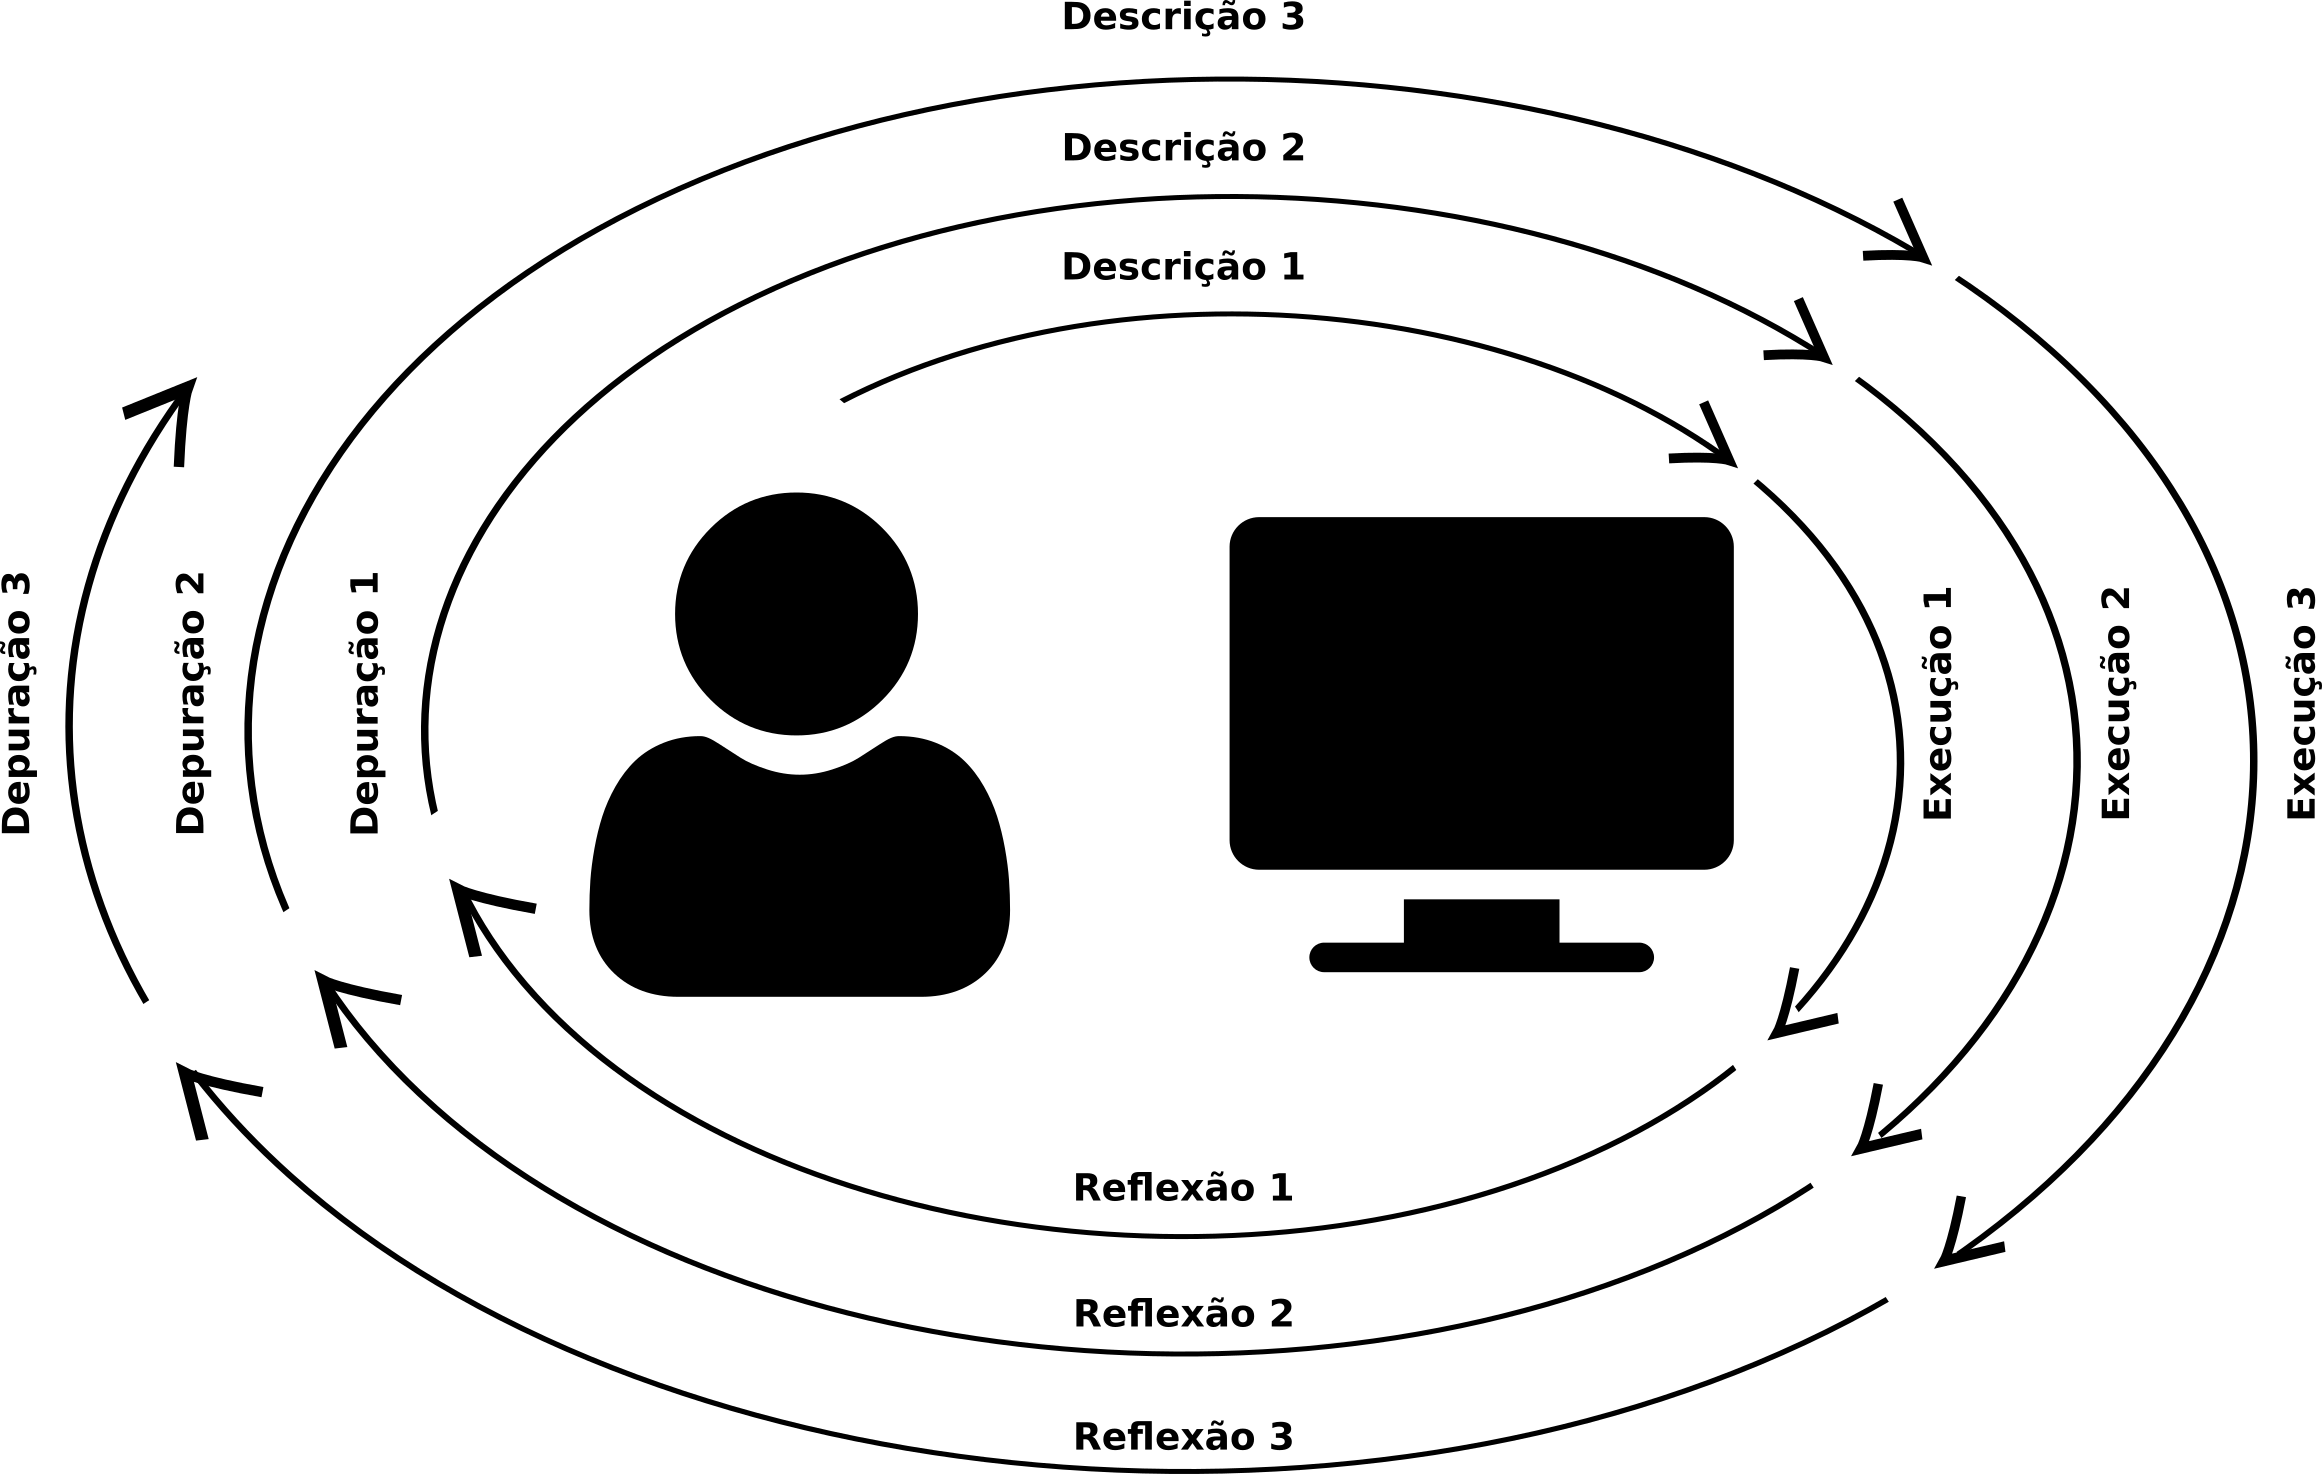
\includegraphics[width=.6\linewidth,fbox]{figs/ciclo_descricao_execucao_reflexao_depuracao.png}
  \caption{Espiral de aprendizagem.}
  \source{Adaptado de \citeonline{valente_aspectos_2018}.}
  \label{fig_espiral}
\end{figure}

A depuração também foi uma das diretrizes de design do ambiente de programação Logo \cite{solomon_history_2020}. Desenvolvido a partir de 1966, ele foi o primeiro ambiente de programação projetado para crianças. Era composto por um computador, uma linguagem textual de programação e um robô com rodas que se movia no chão e desenhava sobre papel. Esse ambiente permitia depurar por meio instruções da própria linguagem, como \textit{pause}, impressão de pilha de comandos e impressão de variáveis. 

Além desses recursos técnicos, para \citeonline{solomon_history_2020} a "grande ideia"\ do Logo era permitir à criança depurar seu próprio entendimento do processo computacional e do algoritmo a ser implementado. Um exemplo é o entendimento dos comandos \textit{left} e \textit{right}, que as crianças confundiam com mover para o lado. Para auxiliar a criança depurar esse conceito, um professor poderia sugeri-la "brincar de ser programada", para então compreender que esses comandos representam movimentos de giro.

A ideia de que a depuração poderia representar uma atividade benéfica para o desenvolvimento cognitivo, somada à existência da linguagem Logo, estimulou pesquisas sobre a prática de depuração por crianças. \citeonline{carver_assessing_1986} avaliaram a depuração de algoritmos por crianças de 7 a 8 anos durante um curso usando Logo. Para isso definiram um modelo de depuração em quatro fases: (i) identificação da diferença entre resultado esperado e resultado obtido; (ii) levantamento de hipóteses para a causa do erro; (iii) localização do \bug\ no código; e (iv) correção do \bug. Com base neste modelo, os pesquisadores concluíram que, após 24 horas de curso, as crianças não desenvolveram estratégias efetivas de depuração, preferindo apagar todo o código e escrever novamente. Posteriormente os mesmos autores conseguiram identificar que crianças aprenderam procurar erros e transferiram esta habilidade para atividades não relacionadas à programação \cite{carver_improving_1987}.

Além de possibilitar pesquisas sobre como as crianças programam, o ambiente Logo contribuiu para o surgimento, na década de 1990, de um ramo de estudos de \ac{IHC} focado no design de interação para crianças \cite{hourcade_child-computer_2015}. Esse ramo de estudos permitiu identificar dificuldades que as crianças tinham ao usar teclado de computadores convencionais \cite{mcnerney_turtles_2004}, projetados para adultos. O uso dos teclados exigia alfabetização, coordenação motora fina, e propiciava a ocorrência de erros sintáticos. Esses aspectos desviavam a atenção que deveria estar focada na construção de algoritmos e entendimento do problema para aspectos secundários, como entender o funcionamento da interface.

O reconhecimento dessa inadequação na interação das crianças com o ambiente de programação, motivou a criação de uma classe de ferramentas dos \ac{BPs}. Os \ac{BPs} descendem do ambiente Logo e buscam facilitar o aprendizado de programação pelo público infantil. Assim como o robô do ambiente Logo, eles geralmente se movem sobre o chão, e tem aparências que remetem ao imaginário infantil, como animais, carros ou robôs \cite{raabe_2017_rope}. Em geral, sua principal funcionalidade é possibilitar à criança inserir comandos, que o brinquedo então executa. Esses brinquedos têm interfaces de programação projetadas para facilitar à criança concentrar-se nos conceitos fundamentais, sem se distrair com erros que não contribuem para o aprendizado de algoritmos.

As interfaces dos \ac{BPs} são simplificadas, para que crianças pequenas saibam como interagir. Adicionar controles de depuração nessas interfaces aumenta a sua complexidade. Ambientes de desenvolvimento profissionais e/ou voltados para o ensino de programação introdutória para adultos apresentam controles de depuração. Esses ambientes mostram valores de variáveis, permitem executar passo a passo e definir pontos de parada \cite{noschang_portugol_2014}. Se adultos precisam destas ferramentas, será que as crianças poderiam se beneficiar das mesmas funcionalidades caso aplicadas em interfaces de \ac{BPs}?

 \citeonline{sipitakiat_robo-blocks_2012} tentam responder essa pergunta ao criar o Robo-Blocks, uma interface tangível de programação em blocos que permite execuções passo a passo. Os autores perceberam que as crianças implementavam “grosseiramente” suas ideias para ver o robô executá-las, sem refletir e aprender com os erros. Além disso, os movimentos rápidos do robô não permitiam comparar as ações do brinquedo com os blocos de “código”, dificultando associar um movimento errado com um bloco. Neste sentido, a execução passo a passo permitiu associar blocos com movimentos, o que foi auxiliado por um LED ativado em cada bloco durante sua execução. 
 
O Cubetto \cite{anzoategui_cubetto_2017} (\autoref{fig_cubetto}) é um \ac{BP} é programado por um painel onde são encaixados blocos de madeira. O painel destaca cada bloco executado acendendo LEDs. Permite, portanto, que a criança associe o movimento do brinquedo com sua causa na lista de comandos. Diferente do Robo-Blocks, porém, não há a opção de execução passo a passo. O Cubetto e o Robo-Blocks, portanto, tentam atacar o problema da depuração em interfaces que devem ser compreendidos por crianças.

Uma característica comum nestes trabalhos é a presença de componentes eletrônicos. Eles têm baterias, conectores e placas eletrônicas. Como alternativa, \citeonline{fincher_tangible_2019} apresentam as “linguagens externamente compiladas”. Elas são interfaces com blocos tangíveis que contém marcas especiais, denominadas marcas fiduciais. Essas marcas são lidas por um sensor óptico e interpretadas por um software que identifica as marcas e as converte em um conjunto de comandos para o brinquedo executar. Deste modo os blocos não carecem de componentes eletrônicos, aumentando a liberdade para os projetistas escolherem os materiais ou objetos a utilizar \citeonline{fincher_tangible_2019}. O KIBO \cite{sullivan_kibo_2015} (\autoref{fig_kibo}) é um executado de \ac{BP} programado por uma linguagem externamente compilada.

\begin{figure}[!htbp]
    \centering
    \begin{subfigure}{.5\textwidth}
        \centering
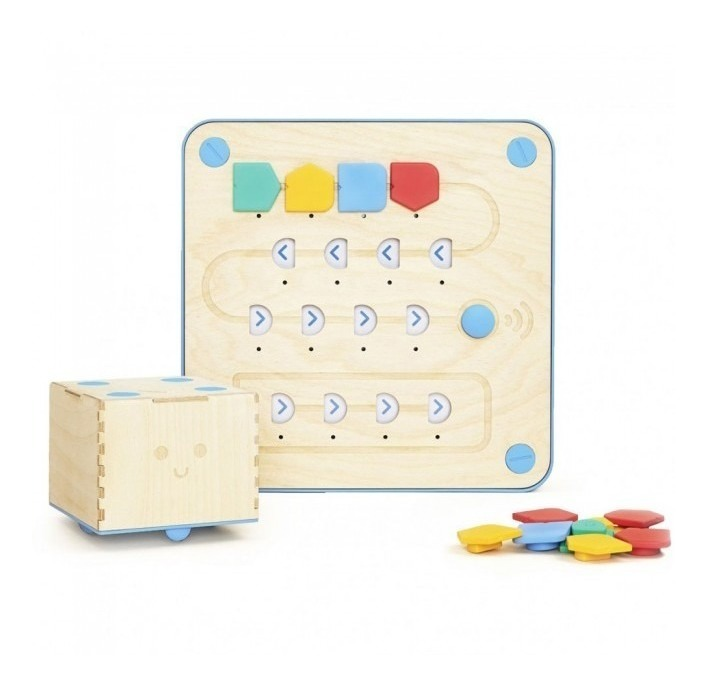
\includegraphics[width=.9\linewidth,fbox]{figs/cubetto.jpg}
        \caption{Cubetto}
        \label{fig_cubetto}
    \end{subfigure}%
    \begin{subfigure}{.5\textwidth}
        \centering
        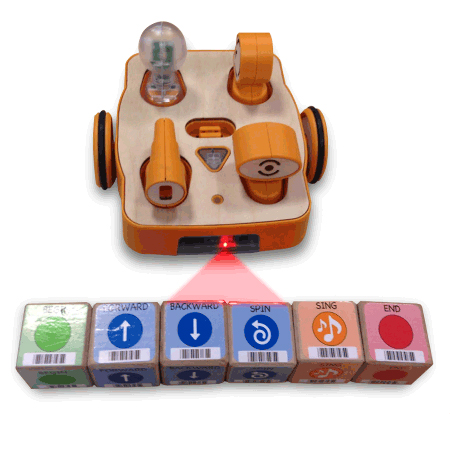
\includegraphics[width=.9\linewidth,fbox]{figs/kibo_2.jpeg}
        \caption{KIBO}
        \label{fig_kibo}
    \end{subfigure}
    \caption{Brinquedos com interfaces tangíveis.}
    \label{fig_toys_tangible}
\end{figure}

Por outro lazo, sem componentes eletrônicos, como LEDs, os blocos tangíveis carecem de meios para representar as instruções do algoritmo que durante a sua execução. A ausência de um indicador dificulta para a criança relacionar o comando está sendo executado e seus efeitos no comportamento do brinquedo. Portanto, também dificulta encontrar causas de erros, bem como mapear símbolos (imagens presente nos blocos) ações (movimentos do brinquedo).

Uma abordagem possível para diminuir a necessidade de eletrônicos também possibilitar indicadores luminosos na interface de programação é \ac{RA} projetiva \cite{roberto_dynamic_2013}. Elá é uma técnica de projeção de elementos virtuais associados a objetos reais. Ela permite que um projetor crie animações, luzes, ou qualquer objeto graficamente representável e os projete interagindo com objetos reais em uma cena. Permite, portanto, avançar a representação oferecida por LEDS fixos em blocos e painéis, ao variar as cores e formas projetadas. Deste modo, os blocos tangíveis do algoritmo podem ser construídos com materiais diversos e ainda assim proporcionar \textit{feedbacks imediatos} \cite{norman_design_1990} durante a depuração.

O RoPE (Robô Programável Educacional) representa uma oportunidade para testar a viabilidade desta abordagem de criação de interfaces tangíveis externamente compiladas e com uso de RA projetiva. Ele é um BP desenvolvido na Univali pelo Laboratório Lite\footnote{\url{https://lite.acad.univali.br}} com foco em crianças a partir dos 3 anos. A sua interface de programação são botões coloridos (\autoref{fig_rope}), desenhados para serem simples de usar por crianças pequenas \cite{raabe_2017_rope}. Essa interface se mostrou um sucesso, e o brinquedo já foi usado em Centros de Desenvolvimento Infantil por mais de 1000 crianças. Além dos botões, pesquisas desenvolveram protótipos de outros modos de interação, como um aplicativo de celular \cite{viana_cesar_interface_2018} e uma interface de programação em similar ao Cubetto \cite{metzger_desenvolvimento_2018}.

\begin{figure}[!htbp]
    \centering
    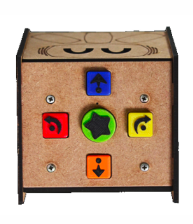
\includegraphics[width=.3\linewidth,fbox]{figs/rope_top.png}
    \caption{Brinquedo RoPE.}
    \label{fig_rope}
\end{figure}

Este trabalho ocorre como uma continuidade dessas e busca contribuir com a área de Informática na Educação ao (1) projetar uma interface tangível externamente compilada para o brinquedo RoPE e (2) explorar o uso de RA projetiva para facilitar a depuração. Essa contribuição se fundamenta na literatura sobre interfaces tangíveis para crianças \cite{sapounidis_evaluating_2015, fincher_tangible_2019, plowman_interactivity_2004} e na observação de que o uso de RA projetiva é um campo pouco explorado no contexto de BPs.

\section{Problema de Pesquisa} \label{s_cintro_problema_pesquisa}

O problema que este trabalho se propõe a investigar no contexto do brinquedo RoPE se insere no que \citeonline{norman_design_1990} denomina falta de \textit{visibilidade}. A visibilidade é um princípio de design relacionado a como o usuário percebe estado de um sistema, e como ele mapeia as ações que pode fazer e que alterações de estado elas provocam.

Em BPs que possuem apenas botões, como a Bee-Bot, o algoritmo que a criança programa não é visível. A criança não vê a sequência de comandos construída ao apertar os botões. Essa invisibilidade dificulta conversar sobre o algoritmo, analisá-lo, encontrar erros e desfazer operações. \citeonline{raabe_brinquedos_2015} menciona esse a incompreensão do funcionamento do botão de limpar a memória da Bee-Bot. As crianças esqueciam de limpar os comandos programados anteriormente, dado que essa ação não é automática. O estado do sistema não é visível, e a criança não sabe se os comandos foram limpos. A solução sugerida foi adicionar um visor de comandos.

No caso das interfaces de blocos tangíveis externamente compiladas (como a utilizada pelo KIBO), o problema é a \textit{invisibilidade de execução} do algoritmo. Os blocos carecem de indicadores que mostrem qual bloco está sendo executado em cada momento, correspondente a cada movimento do brinquedo. Essa falta de visibilidade de execução dificulta compreender a sequência lógica de funcionamento do algoritmo, pois não há mapeamento entre comando/bloco e ação do robô. O Cubetto soluciona esse problema através de luzes indicadoras, e para isso depende de um painel onde os blocos são encaixados.

\citeonline{norman_design_1990} comenta que dispositivos cujas interfaces não demonstram o estado interno durante a interação podem influenciar o entendimento do usuário sobre como tal dispositivo funciona. Esse “entendimento” é denominado modelo mental. Caso o dispositivo executar de forma inesperada, o usuário tende a encontrar alguma explicação para justificar tal comportamento. Ao justificá-lo, cria um modelo mental incorreto. \citeonline{raabe_brinquedos_2015} apresentam crianças justificando comportamentos inesperados da Bee-Bot após terem esquecido de limpar sua memória, afirmando que a “abelha” tinha vontade própria.

Por fim, essa falta de visibilidade desencadeia a dificuldade em depurar. A literatura \cite{carver_assessing_1986, mccauley_debugging_2008} apresenta modelos organizam a ação de depurar em etapas, entre as quais está a de localizar e reparação erros em algum código-fonte. A ausência do código-fonte, portanto, impede a depuração segundo estes modelos.

Partindo destas reflexões, elaborou-se a seguinte pergunta de pesquisa: 
\textit{como crianças de 4 a 6 anos interagem com uma interface de programação focada em permitir visualizar os passos e a execução de um algoritmo?}

\begin{comment}
    \begin{quadro}[!htbp]
 \caption{Vantagens e desvantagens de botões, cartas, tangíveis e aplicativos}
 \label{quadro_vantagem_desvantagem} 
 \begin{center}
 \begin{footnotesize} 
\begin{tabular}{|p{3cm}|p{3cm}|p{4.5cm}|p{4.5cm}|}
\hline
Tipo de interface & Exemplos            & Vantagens & Desvantagens\\ \hline
Botões            & RoPE, Bee-Bot       & - Facilidade de inserir comandos & - Não mostra algoritmo. \newline 
                                                                             - Não permite editar comandos, somente apagar tudo e recomeçar.
\\ \hline
Cartas            & Bee-Bot, \newline
                    Go-Robot Mouse      & - Baixo custo \newline                
                                          - Permite colaboração \newline
                                          - Customizável \newline           & - Falta de sincronia \newline 
\\ \hline
Aplicativos       & Dash, Sphero        & - Sincronia \newline 
                                          - Baixo Custo \newline
                                          - Replicabilidade \newline
                                          - Depuração \newline              & - Tempo de tela \newline
                                                                              - Difícil colaboração

\\ \hline
Blocos tangíveis  & Cubetto, KUMIITA    & - Experiência sensorial
                                          - Colaborativo \newline   
                                          - Algoritmo visível \newline      & - Custo
\\ \hline
                                        
\end{tabular}
 
 \end{footnotesize}
 \end{center} 
 \sourceauthor
\end{quadro}
\end{comment}

\subsection{Solução Proposta}
\label{ss_cintro_solucao}

A proposta é desenvolver uma interface de \ac{RA} projetiva combinada com uma linguagem externamente compilada. Dado que os blocos de linguagens externamente compiladas tem marcas fiduciais, uma câmera pode captar as posições dos blocos e um algoritmo pode controlar um projetor para destacá-los \autoref{idea}.

\begin{figure}[!htpb]
  \centering
  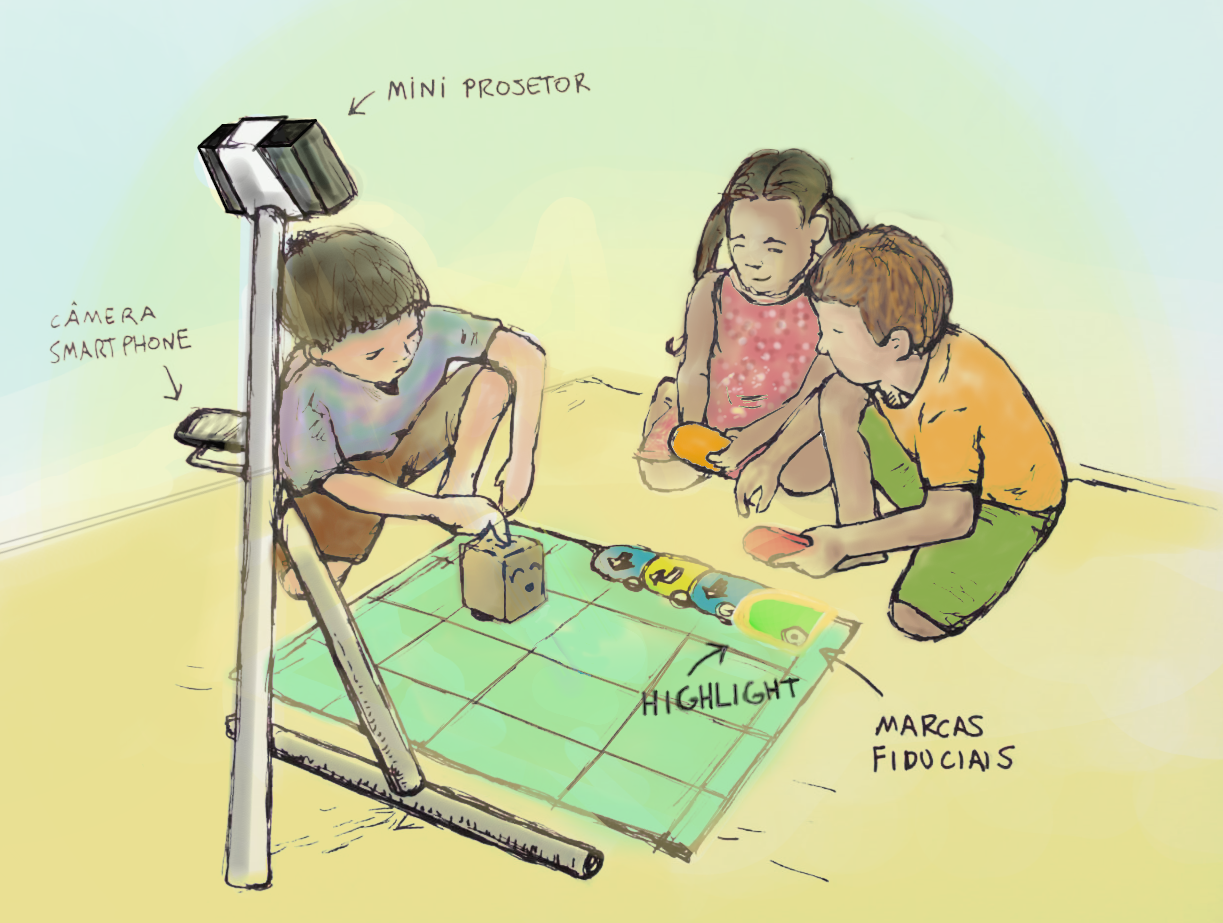
\includegraphics[width=.85\linewidth,fbox]{figs/idea_2.png}
  \caption{Solução proposta: interface tangível com realidade aumentada.}
  \sourceauthor
  \label{idea}
\end{figure}

A intenção é que a criança programe utilizando blocos de papelão com símbolos de setas correspondentes às ações do RoPE. Um \textit{smartphone} é usado como câmera, pois é mais acessível e fácil de manusear do que um notebook ou desktop. Um projetor portátil, de baixa potência de iluminação (1200 lumens) e de baixo custo ilumina os blocos e projeta um mapa interativo.

Outra funcionalidade implementada é o estado de \textit{execução passo a passo}. Ao ativar esse estado o brinquedo executa um comando e espera a criança disparar a execução da próxima ação. Isso possibilita à criança mais tempo para olhar cada bloco e compreender o movimento associado a ele. A intenção é que a criança possa compreender possíveis erros no algoritmo construído por ela ou por outra criança.

A partir do uso de RA e de um estado de execução passo a passo, a proposta é possibilitar um melhor entendimento, por parte da criança, a respeito do algoritmo que ela está construindo, e sobre seu próprio modo de pensar. Esta abordagem é exploratória, e não foram encontrados dados quantitativos passíveis de comparações numéricas com outros estudos. Este trabalho, portanto, apresenta a construção da proposta e a avaliação qualitativa das interações de crianças de 4 a 6 anos com a mesma.

\subsection{Delimitação de Escopo}
\label{ss_cintro_escopo}

Este trabalho é sobre uma ferramenta para facilitar o aprendizado de algoritmos por crianças. Algoritmos é um dos quatro pilares do \acl{PC} \cite{brackmann_desenvolvimento_2017}, junto à decomposição, abstração e reconhecimento de padrões. Este trabalho cita definições destes pilares, porém a solução proposta tem foco apenas em algoritmos, e, mais especificamente, na atividade de depurá-los.

Não é objetivo deste trabalho realizar testes com comprovação estatística, no sentido de identificar relações de causa e efeito no aprendizado. O foco é descrever a presença ou ausência das dificuldades mais perceptíveis durante a interação com uma ferramenta educacional. Esse foco se adequa à pesquisa de cunho qualitativo, com um número reduzido de crianças.

Também não foi objetivo programar um algoritmo de visão computacional para reconhecer os blocos tangíveis e o RoPE. Uma biblioteca de identificação de marcas fiduciais permitiu agilizar a implementação de um protótipo funcional. A eliminação de marcas fiduciais poderá ocorrer em trabalhos futuros, considerando os aprendizados obtidos com a primeira versão aqui apresentada.

% ----------------------------------------------------------------------- %
\subsection{Justificativa}
\label{ss_cintro_justificativa}

O mapeamento industrial descrito no \autoref{c_estado_arte}, demonstra que, de 56 brinquedos, apenas 2 utilizam RA. Ainda assim o seu uso ocorre através de tablets e celulares, menos indicados para crianças em comparação com as interfaces tangíveis \cite{sapounidis_tangible_2019, zuckerman_tui_2013}.

No mesmo mapeamento, o RoPE aparece como o único projeto brasileiro em atividade voltado ao ensino de programação para crianças pequenas com brinquedos programáveis. Desde a sua concepção, o projeto estuda aspectos de design para que crianças possam aprender de forma lúdica e evitando erros não construtivos \cite{raabe_brinquedos_2015}. A abordagem aplicando \ac{RA}, como este trabalho propõe, ainda não foi experimentado com o RoPE ou outros brinquedos. Considerando o pioneirismo do RoPE como ferramenta educacional para aprendizado de algoritmos por crianças no Brasil, entende-se que a exploração proposta neste trabalho pode contribuir com novas informações para o projeto.

A reprodução da proposta é facilitada pelo fato da mesma não utilizar componentes eletrônicos específicos. Os componentes usados são produtos disponíveis comercialmente, que precisam ser plugados (mini-projetores, \textit{smartphones} e Arduino). O RoPE compartilha princípio de ser programado por botões com diversos outros brinquedos, como a Bee-Bot, Go Robot Mouse e Thymio. Esses brinquedos também poderiam ser aplicados no contexto da proposta, o que também facilita sua reprodução.

A proposta de usar \ac{RA} projetiva abre caminho para desenvolver tapetes dinâmicos. Atualmente o brinquedo RoPE se move sobre tapetes estáticos, que precisam ser trocados conforme a atividade. A projeção, associado à informação da localização do brinquedo, permite disparar eventos quando este atinge determinadas posições. Esses eventos viabilizam a construção de jogos, em que as fases avançam conforme os movimentos do brinquedo. Portanto, ao permitir que um sistema computacional perceba a posição do brinquedo e projete o ambiente, surgem novas possibilidades de interação.

Novas possibilidades de interação também surgem ao utilizar a programação em blocos. Por estarem desassociados dos botões do RoPE, os blocos podem expandir as funções já existentes sem a necessidade de modificações físicas no brinquedo. Enquanto os botões definem ações específicas, como giros de 90.º, adequadas para as crianças iniciarem os primeiros algoritmos, os blocos podem definir outros movimentos, como giros de 45.º, por exemplo. Além disso, outros blocos podem programar eventos de sons e luzes, e também animações como trocar o mapa projetado.

Entretanto, prosseguir com essas possibilidades exige avaliar a ferramenta no em centros de desenvolvimento infantil com crianças de 4 a 6 anos. Essa avaliação é necessária por dois motivos principais. Primeiro, obter a opinião de professores e crianças sobre a interface; e segundo, verificar riscos, como a criança obstruir as marcas fiduciais, ou os elementos físicos e virtuais representarem uma fonte de distração e não de aprendizado.

Por fim, a proposta está ligada a uma área de interesse da comunidade científica\footnote{Possui jornais dedicados ao tema, como International Journal of Child-Computer Interaction e ACM Transactions on Computer-Human Interaction.}, e ao fato de que há uma lacuna de compreensão sobre utilização de \ac{RA} projetiva com brinquedos programáveis.

\section{Objetivos}
\label{s_cintro_objetivos}

\subsection{Objetivo Geral}
\label{ss_cintro_objetivo_geral}

Avaliar qualitativamente o uso de uma interface de \ac{RA} projetiva na depuração de algoritmos do brinquedo RoPE por crianças de 4 a 6 anos.

\subsection{Objetivos Específicos}
\label{ss_cintro_objetivos_espec}

Os objetivos específicos do trabalho são:

\begin{enumerate}
    
    \item Relacionar sistemas e aplicações que utilizam realidade aumentada projetiva;

    \item\label{obj_mapear} Categorizar as interfaces de brinquedos programáveis existentes;

    \item\label{obj_interface} Construir a interface de realidade aumentada projetiva para o brinquedo RoPE;

    \item\label{obj_avaliar} Aplicar a interface em atividades com crianças para coletar e analisar eventos de interação.
    
\end{enumerate}
\section{Metodologia}
\label{s_cintro_metodologia}

Esta seção descreve a metodologia e os procedimentos metodológicos utilizados nesta pesquisa.

\subsection{Métodos da Pesquisa}
\label{ss_cintro_metod_pesquisa}

Métodos científicos são conjuntos de procedimentos técnicos adotados para produzir conhecimento \cite{gil_metodos_2008}, construído através de passos para atingir os objetivos de uma pesquisa \cite{wazlawick_metodologia_2009}. O método desta pesquisa pode ser descrito como de natureza aplicada, pois prevê a aplicação prática de uma ferramenta e tecnologias para solucionar um problema de interação com brinquedos programáveis. A abordagem sobre o problema foi qualitativa, ao observar aspectos subjetivos como falas, gestos e expressões durante o uso da solução proposta. Por fim, esta pesquisa é exploratória, ao buscar extrair informações de um fenômeno desconhecido, a partir de uma pequena amostra de participantes em caráter experimental. A próxima subseção descreve os procedimentos metodológicos adotados.

\subsection{Procedimentos Metodológicos}
\label{ss_cintro_proced_metodologicos}

A construção da solução proposta e atendimento dos objetivos de pesquisa possui quatro fases: estudo, modelagem, implementação e avaliação, descritas a seguir.

\begin{description}
    \item[Estudo] Essa etapa correspondeu a uma revisão sistemática, um mapeamento industrial e um levantamento de trabalhos similares. A revisão sistemática focou em compreender como são feitas pesquisas científicas avaliando interfaces de programação de brinquedos programáveis. O mapeamento buscou descrever as categorias de interfaces mais utilizados em projetos de brinquedos programáveis, incluindo produtos comerciais. Por último, trabalhos similares descrevem o uso de projeção ou formas de facilitar a programação por crianças.

    \item[Modelagem] A etapa de modelagem ocorreu como um planejamento dos elementos de software a serem implementados. Esta etapa envolveu levantamento de requisitos (\autoref{apendice_requisitos}) e prototipação (\autoref{apendice_prototipo}) para conferir a viabilidade da proposta. 

    \item[Implementação] Etapa que correspondeu a programar o aplicativo (i) alterar o \textit{firmware} do brinquedo RoPE para comunicação sem fio; (ii) configurar a conexão com uma plataforma de armazenamento das interações ocorridas com um brinquedo programável; (ii) adaptar o \textit{firmware} do RoPE para comunicação sem fio; e (iii) programar um aplicativo de \textit{smartphone} para captar os blocos e comunicar com o projetor.
   
    \item[Avaliação] A avaliação\footnote{Para atendimento do objetivo específico \autoref{obj_avaliar}.} aqui compreendida na observação de crianças em atividades de programação do RoPE, para coletar e por fim analisar dados seguindo um protocolo definido no \autoref{c_avaliacao}. Essa etapa envolveu aplicação do software de  análise qualitativa Qualcoder, para tratamento dos dados coletados. 

\end{description} 

\section{Estrutura da Dissertação}
\label{s_cintro_estrutura}

O trabalho está organizado em 6 capítulos correlacionados. O \autoref{c_introducao}, contextualizou e apresentou o tema, o problema e uma proposta de como solucioná-lo. Foram estabelecidos os objetivos a serem alcançados com a solução, e as limitações de escopo a serem observadas.

O \autoref{c_fundamentacao_teorica} apresenta a fundamentação teórica iniciando com a descrição do sujeito desta pesquisa (a criança) e observa fundamentos relacionados ao desenvolvimento infantil. Como tema relacionado a algoritmos, é apresentada a definição de \ac{PC} em quatro pilares. O capítulo também apresenta fundamentos sobre as interfaces de brinquedos programáveis, bem como aplicações de realidade aumentada projetiva.

O \autoref{c_estado_arte} apresenta o estado da arte em três aspectos: das pesquisas realizadas com brinquedos programáveis; interfaces de brinquedos mais utilizados no mercado; e trabalhos com semelhanças tecnológicas e conceituais.

\autoref{c_desenvolvimento} é o quarto capítulo, que apresenta uma visão geral dos componentes da contribuição: aplicativo e elementos tangíveis. O capítulo apresenta aspectos técnicos da implementação, tecnologias utilizadas para construir esses componentes e possibilitar a comunicação entre os mesmos.

O \autoref{c_avaliacao} descreve o contexto de execução da pesquisa. Ele também apresenta o protocolo de teste e os instrumentos de coleta usados durante atividades com crianças. Em seguida, o \autoref{c_resultados} apresenta os resultados obtidos com a análise dos dados coletados.

Por fim, o \autoref{c_conclusao} revisa o atendimento aos objetivos da pesquisa, reflete sobre as contribuições geradas e propõe trabalhos futuros.
\chapter{Fundamentação Teórica}
\label{c_fundamentacao_teorica}

Este capítulo discute os principais temas de interesse desta pesquisa, iniciando pelo sujeito principal: a criança. As bases teóricas são as teorias do Construtivismo e do Construcionismo, e os autores são Jean Piaget, Seymour Papert e Jerome Bruner. A \autoref{fundamentacao_pc} apresenta a definição de \ac{PC} que esta pesquisa segue. Depois o texto apresenta ferramentas voltadas ao aprendizado de algoritmos por crianças, como os brinquedos programáveis.

\section{A criança}
\label{fundamentacao_crianca}
No Brasil, o Estatuto da Criança e do Adolescente considera como criança a pessoa de até 12 anos incompletos \cite{brasil_lei_1990}, porém \citeonline{markopoulos_evaluating_2008} afirma que a duração da infância é relativa a influências culturais, localização e base familiar. O desenvolvimento cognitivo da criança desde o nascimento até a idade adulta foi um dos temas de pesquisa de Piaget, que posteriormente influenciou as pesquisas de Seymour Papert, criador do ambiente Logo.

A importância de compreender como as crianças aprendem é fundamental para criação de ferramentas educacionais. \citeonline{rogers_design_2013} afirmam que projetar experiências interativas que atendam as necessidades dos usuários passa por entendê-los nos contextos em que vivem, trabalham e aprendem. A observação cuidadosa do indivíduo pode revelar opiniões incorretas, por parte dos designers, sobre o que um grupo pode necessitar ou desejar. Quando o público-alvo do produto interativo é composto por crianças é ainda mais difícil para designers adultos preverem o que pode ser adequado e simples de usar.

Por isso esta seção apresenta teorias de aprendizado de Jean Piaget, Jerome Bruner e Seymour Papert. Esses autores buscaram compreender como o conhecimento se forma na mente da criança, e como materiais externos podem auxiliá-la a aprender melhor. \citeonline{gray_learning_2015} apresenta uma visão completa de teorias de aprendizagem, mas os autores aqui apresentados se justificam pela influência que tiveram no campo da tecnologias educacionais para crianças.

%A tentativa de compreender o indivíduo enquanto criança está presente no trabalho de pesquisadores como Maria Montessori, Jean Piaget e Seymour Papert. Montessori foi uma médica italiana que desenvolveu desde 1907 uma experiência de ensino chamada \textit{Casa dei Bambini}\footnote{Casa das Crianças.}, fortemente atenta à qualidade do ambiente infantil, com materiais acessíveis e capazes de promover aprendizado por meio de experiências sensoriais. Nesse método a criança interagia com ferramentas que a estimulavam a desenvolver o raciocínio, e Montessori desenvolveu estas ferramentas ao dedicar atenção às necessidades das crianças em vez de tratá-las como pequenos adultos. Os materiais desenvolvidos e aplicados por Montessori são utilizados até hoje em ambientes educacionais infantis.

\subsection{Piaget e o Desenvolvimento Cognitivo}
Piaget estudou o desenvolvimento cognitivo da criança e propôs a teoria denominada Epistemologia Genética. Essa teoria une as correntes filosóficas do apriorismo e do empirismo. Enquanto o apriorismo preconiza que todo conhecimento é inato, ou seja, existe no ser humano desde o nascimento, o empirismo defende que o aprendizado e o conhecimento surgem das interações do sujeito com seu meio. Piaget concorda com o empirismo ao afirmar que o conhecimento surge das experiências e também concorda com o apriorismo quando diz que o aprendizado depende de estruturas mentais capazes de assimilar essas experiências.

A partir disso, Piaget descreveu o aprendizado como um processo de assimilação e acomodação. A criança nasce com poucas estruturas mentais (esquemas), e ao receber estímulos motores, conceituais ou perceptuais, tenta classificá-los e assimilá-los de acordo com aquilo que já conhece. Por exemplo, ao ver um cachorro pela primeira vez a criança pode assimilá-lo como sendo outro animal semelhante para o qual já tenha um esquema criado. Ao ser corrigida por um adulto, porém, um novo conceito surge e precisa ser acomodado, criando assim um novo esquema.

Além de descrever o processo de aprendizado, o pesquisador descreve etapas de desenvolvimento cognitivo. Cada estágio se caracteriza pelo modo como a criança realiza determinadas operações mentais. A realização de uma “operação” significa executar uma ação mental que tem reversão e conservação. Um exemplo de reversão e conservação é observar que um líquido transvasado de um recipiente maior para outros dois recipientes menores mantém sua quantidade total e pode retornar ao recipiente maior sem mudança de volume. Há reversão pois o líquido pode retornar ao local original, e conservação pois a quantidade final é a mesma da inicial. Piaget demonstrou que crianças não conseguem perceber essa relação e sugeriu que isso se devia à ausência das estruturas mentais necessárias. Neste sentido, o pesquisador seguiu observando quais operações mentais crianças conseguiam executar em cada faixa etária e com isso organizou o desenvolvimento cognitivo em quatro estágios:

\begin{description}
\item[Sensório motor] é o primeiro estágio. Inicia no nascimento e vai até os 18 meses \cite{piaget_development_1964}. Nesta etapa não há conservação: se um objeto some do campo de visão da criança ele deixa de existir para ela. \citeonline{montessori_o_2019} indica não mudar frequentemente o ambiente da criança, para que ela possa identificar a permanência dos objetos.

\item[Pré-operacional] é o estágio que inicia aos 18 meses e vai até os 6 ou 7 anos. Ainda não há estruturas que suportam operações mentais, mas há o aparecimento da linguagem e dos símbolos, o que possibilita o pensar.

\item[Operatório-concreto] é o estágio onde se iniciam as operações. Ele é denominado "concreto" pois as operações dependem de objetos físicos, ou seja, a operação mental precisa estar ligada à uma operação física. Neste período a criança consegue fazer classificações, ordenar objetos e tem a ideia de número.

\item[Operatório-formal] é o último estágio, e vai dos 12 anos até o final da vida. A pessoa consegue raciocinar sobre hipóteses abstratas, impossíveis até de serem concretizadas fisicamente. Há suporte para captar informações fontes variadas e obter conclusões, o que é mais complexo que o raciocínio ligado a ordenação e classificação \cite{piaget_development_1964}.

\end{description}

Percebe-se a partir da descrição do estágio operatório-concreto, a importância de objetos concretos para possibilitar a realização de operações mentais por crianças entre 7 e 12 anos. Segundo Hourcade (2015), a pesquisa de Piaget sobre como a criança aprende afetou fortemente os campos da IHC. A compreensão da importância de materiais concretos até hoje é observável em ambientes educacionais infantis, e no campo das interfaces de programação pode ser melhor observado nas interfaces tangíveis, que permitem à criança programar utilizando objetos físicos.

\subsection{Jerome Bruner: Construtivismo no Ensino}
\label{sub_jerome_bruner}
Assim como Piaget, Bruner foi um psicólogo construtivista e apoiava a ideia de que o conhecimento é construído pelo indivíduo por meio de experiências. Porém, enquanto Piaget se concentrou na aprendizagem, Bruner estudou como melhorar o ensino. Neste sentido, Bruner destaca três aspectos para melhorar o ensino: representação do aprendizado, currículo em espiral e aprendizagem por descobertas.

A representação do aprendizado seria a forma de adquirir e internalizar o conhecimento, e também ocorre em estágios. Há três modos de representação: enativa, icônica e simbólica. A primeira aconteceria com experiências concretas, “mão na massa”, com estímulos sensoriais tangíveis. Um exemplo seria a criança dividir uma laranja em duas partes. Na segunda fase – representação icônica – o aprendiz associa as experiências sensoriais anteriores com imagens e figuras icônicas, ou seja, semelhantes visualmente com aquilo que representam. A figura de uma laranja dividida em diferentes partes é associada com a experiência concreta anterior.

Esse espectro de representação do concreto/sensorial para o abstrato/formal pode traçar um paralelo com as interfaces de programação. A criança precisa ter contato físico, enativo com algo. Esse contato facilita a compreensão do algoritmo por ícones, como usados em programação em blocos virtuais \cite{flannery_designing_2013}, e aos poucos se alcança o uso de linguagens de programação textuais.

O segundo aspecto defendido é o currículo em espiral. Para Bruner, cada atividade de ensino deve repetir as ideias fundamentais lecionadas em uma etapa anterior e adicionar novas camadas de complexidade. À medida que a complexidade aumenta, o aluno tem necessidade de um auxílio, sem o qual pode levar muito tempo para entender determinado conceito. Neste momento entra o papel de um tutor com a informação a ser transmitida, proporcionando o que Bruner denomina \textit{scaffolding}. No \textit{scaffolding} o tutor auxilia o estudante no aprendizado inicial de um conteúdo \cite{valkenburg_joining_2010} e remove a assistência à medida que o aprendiz adquire autonomia. Para isso o tutor \textit{scaffolding} avalia o que o estudante já sabe e trabalha somente as suas dificuldades, garantindo que ele faça a maior parte do trabalho de forma independente \cite{valkenburg_joining_2010}.

Projetar ferramentas que incentivem o \textit{scaffolding} entre adultos e crianças é uma preocupação do campo de design de interação para crianças. \citeonline{plowman_interactivity_2004} observam que a presença de um elemento tangível pode aumentar o número de vezes em que adultos auxiliam crianças. \citeonline{horn_tangible_2012} afirmam que as interfaces tangíveis combinadas com as interfaces gráficas tem o potencial de fornecer \textit{scaffolding} à medida que os estudantes podem transitar de um sistema tangível para sistemas gráficos com recursos e complexidades aumentados. Já \citeonline{catlin_edurobots_2018} comenta o mesmo sobre a robótica educacional:

\begin{citacao}
Robots allow teachers to create environments which reflect Bruner’s Spiral Curriculum [...]. Young children start with [a robot] where all they do is put symbols in the right order, but as their experience and interest grows they can end up coding in professional programming languages. Several robots provide rich educational environments by offering different ways for students to program them \cite{catlin_edurobots_2018}.
\end{citacao}

%\begin{citacao}
%Além dessas vantagens imediatas das interfaces híbridas, está o potencial de fornecer \textit{scaffolding} para os alunos à medida que progridem em direção a ambientes de programação cada vez mais autênticos. Por exemplo, os alunos podem começar com um sistema tangível e depois fazer a transição para um sistema gráfico com recursos e complexidade aumentados. Levando essa ideia adiante, os alunos podem posteriormente fazer a transição de um ambiente de programação gráfica para um ambiente baseado em texto com recursos e capacidades avançadas \cite[p. 388, tradução nossa]{horn_tangible_2012}.
%\end{citacao}

Por fim, Bruner defende o aprendizado por descobertas. Segundo ele, o aprendiz deve estar motivado pela curiosidade. Representar conceitos adequadamente e auxiliar o aprendiz em suas dificuldades são formas de contribuir para que sua curiosidade se transforme em conhecimento.

\subsection{Papert e o Construcionismo}

Outro teórico que estudou o desenvolvimento infantil foi Seymour Papert. Enquanto Piaget e Bruner foram teóricos construtivistas, Papert criou uma nova teoria denominada Construcionismo. Ela tem base no construtivismo de Piaget, com quem Papert trabalhou, e ambas as teorias compartilham a ideia de “construir estruturas de conhecimento” \cite{papert_situating_1991}. A diferença é que Construtivismo se concentra em como as estruturas são construídas na mente do aprendiz, e o Construcionismo foca em como materiais externos podem auxiliar na construção dessas estruturas de conhecimento \cite{bers_blocks_2008}.

O foco nos materiais e ferramentas decorre da crença de que objetos bem projetados possibilitam criar projetos significativos do ponto de vista epistemológico \cite{bers_blocks_2008}. O material deve ter uma finalidade aberta, permitindo exercitar a criatividade. Exemplos desse tipo de material são blocos de encaixar, o computador e a robótica. Eles permitem combinar diferentes partes a fim de testar hipóteses, errar, avaliar e testar novas possibilidades. Essa versatilidade possibilita ao aprendiz criar artefatos do seu interesse, o que aumenta a motivação e a curiosidade assim como a aprendizagem por descobertas proposta por Bruner. \citeonline{papert_teaching_1972} comentava:

\begin{citacao}
Eu acredito com Dewey, Montessori e Piaget que as crianças aprendem fazendo e pensando sobre o que fazem. E, portanto, os ingredientes fundamentais da inovação educacional devem ser coisas melhores para fazer e maneiras melhores de pensar sobre si mesmo fazendo essas coisas \cite[p.3, tradução nossa]{papert_teaching_1972}.
\end{citacao}

A liberdade da programação está em criar blocos de código e combiná-los de infinitas maneiras e gerar infinitos resultados. Percebendo essa harmonia com o Construcionismo, Papert e seu grupo de pesquisa desenvolveram a linguagem LOGO, a primeira linguagem de programação criada para e por crianças \cite{solomon_history_2020}. A linguagem LOGO é conhecida como a "linguagem da tartaruga"\ ao permitir programar um agente para se mover, girar e desenhar. Essa tartaruga pode ser digital, na tela de um computador; ou física, na forma de brinquedos programáveis.

Desde o desenvolvimento do LOGO, pesquisas têm se inspirado nos fundamentos construcionistas para criar ferramentas adaptadas para crianças. Exemplos são ambientes de programação em blocos como o Scratch e o ScratchJr \cite{flannery_designing_2013}, e diversos brinquedos programáveis (ver \autoref{brinquedos_programaveis}). Os ambientes de programação em blocos permitem encaixar blocos de código evitando erros de sintaxe comuns na programação da digitação em teclado, como no caso do LOGO. Já os BPs permitem infinitos programas ainda que com número reduzido de comandos disponíveis. Essas ferramentas carregam os princípios construcionistas de serem fáceis de começar, mas infinitas nas possibilidades de criar, testar hipóteses, e compartilhar criações significativas.

\citeonline{bers_blocks_2008} adaptou os princípios construcionistas para o contexto da Educação Infantil, dos quais dois fundamentam esse trabalho. O primeiro deles é \textit{"Usar objetos concretos para construir e explorar o mundo"}. O estágio operatório concreto proposto por Piaget menciona a necessidade que crianças têm de utilizar objetos concretos para realizar operações mentais. Crianças precisam se engajar em atividades com objetos reais, com manipulação de brinquedos que as façam pensar. O modo de interação mais proeminente neste sentido são as interfaces tangíveis. O segundo princípio é \textit{"Engajar em autorreflexão como parte do processo"}. O processo de depurar algoritmos representa essa reflexão, ou seja, o momento que a criança pensa sobre aquilo que criou. Ao encontrar um \bug, ocorre então o processo de acomodação, ou seja, o resultado não se "encaixa" nos esquemas existentes na mente da criança e precisa ser acomodado. A criança pode então alterar o algoritmo, e ao executar novamente, perceber se o resultado pode ser assimilado pelo esquema mental recém criado, confirmando ou refutando-o.
    
\begin{comment}
    \citeonline{bers_blocks_2008} lista quatro princípios do Construcionismo que se adaptam à Educação Infantil.
    \item Aprender criando projetos significativos e pessoais para compartilhar com a comunidade;
    \item Usar objetos concretos para construir e explorar o mundo;
    \item Identificar ideias poderosas do domínio de estudo;
\end{comment}

As teorias apresentadas nesta seção representam apenas um recorte da teoria existente, e buscou focar em aspectos ligados ao tema de ferramentas educacionais. O Construcionismo é uma filosofia centrada em apoiar a liberdade do aprendiz, e para isso propõe o uso de ferramentas poderosas que o auxiliem a criar e a pensar sobre essas criações. A programação é uma dessas ferramentas e tem o poder de permitir o exercício da criatividade e autonomia por parte do estudante. A programação se dá por meio de diferentes interfaces, e o seu desenvolvimento seguindo princípios fundamentados em teorias como o construcionismo já ocorre desde a linguagem Logo. Esses princípios têm como influência o construtivismo de Piaget, que apontou a necessidade de materiais concretos para apoiar o raciocínio. Neste sentido, os princípios do currículo em espiral de Bruner também influencia a construção de brinquedos de modo que possuam interfaces de programação com níveis crescentes de poder e complexidade. Exemplos são apresentados na \autoref{secao_mapeamento_industrial}.

%\subsection{Noção de Espaço na Criança: Localização e Direção}
%Reconhecer e comunicar informações sobre espaços é atividade constante do ser humano. Para \citeonline{ferrara_2011}, habilidades espaciais são cruciais para o intelecto humano, pois estão ligadas a atividades como pensar em escalas de objetos, compreender como chegar a um destino, e transformar mentalmente informações. Os campos de engenharia e matemática dependem muito desse tipo de raciocínio. \cite{piaget_representacao_1981} mencionam que o ensino da geometria poderia ganhar muito ao compreender a evolução das noções de espaço da criança.

%\citeonline{cannon_system_2007} definem 8 categorias de palavras para comunicar noções espaciais, incluindo dimensões, formas, locais e direções, orientações e transformações e quantidades. Palavras referentes a direções sã

% importância do espaço
%   O ensino da geometria poderia ganhar muito ao adaptar-se à evolução espontânea das noções [de espaço]. Piaget (1981).
%  Spatial skills are crucial to intellect, transformação mental, STEM.

% diferentes noções de espaço (posição, tamanho, forma)
% localização e direção
% três montanhas

%How do spatial skills develop? One important answer may lie in the relationship between human spatial cognition and the symbol systems we use to describe spatial concepts. Ferrara


\section{Pensamento Computacional}
\label{fundamentacao_pc}
%Existem múltiplas definições de \acl{PC} \cite{barr_bringing_2011}. Ressaltam aspectos..

O \acl{PC} é um termo utilizado inicialmente por \citeonline{papert_mindstorms:_1980}, mas que tem recebido maior atenção a partir de 2006, quando Jeannette Wing publicou o artigo opinativo intitulado "Computational Thinking"\ na revista \textit{Communications of the ACM} \cite{wing_computational_2006}. No artigo, Wing define o \ac{PC} como “[...] conjunto de atitudes e habilidades universalmente aplicáveis que todos, não apenas os cientistas da computação, estariam ansiosos por aprender e usar” \cite[p.33, tradução nossa]{wing_computational_2006}. Considerando essa universalidade de aplicações, Wing afirma que o \ac{PC} deve ser aprendido pelas crianças assim como a escrita, leitura e matemática. Em trabalhos posteriores a autora menciona que o \acl{PC} é um processo de pensar um problema de forma a admitir uma solução computacional. Essa solução pode ser gerada por uma máquina, por um humano, ou pela combinação de ambos. Em 2014, Wing acrescenta que o \ac{PC} não trata apenas de como resolver problemas, mas também de como formulá-los \cite{wing_computational_2014}.

\citeonline{barr_bringing_2011} afirmam que uma definição de \ac{PC}, para ter utilidade, precisa trazer exemplos de como incorporá-lo aos ambientes educacionais. Neste sentido, em 2009 aproximadamente 700 professores da \ac{ISTE} ISTE (\textit{International Society for Technology in Education} -- Sociedade Internacional para Tecnologia na Educação) e da \ac{CSTA} desenvolveram, em 2011, uma “definição operacional”\ do \acl{PC}. Essa definição caracteriza o \ac{PC} como um processo de resolução de problemas, que inclui (mas não se limita) a:

\begin{itemize}
    \item Formular problemas de forma que um computador possa auxiliar a resolvê-los;
    \item Organizar e analisar dados logicamente;
    \item Representar dados por meio de abstrações, como modelos e simulações;
    \item Automatizar soluções por meio de pensamento algorítmico (série de passos ordenados);
    \item Identificar, analisar e implementar possíveis soluções com o objetivo de alcançar a combinação mais eficiente e eficaz de processos e recursos;
    \item Generalizar e transferir o processo de solução do problema para outros problemas.
\end{itemize}

\citeonline{brackmann_desenvolvimento_2017}, a partir da definição de \citeonline{bbc_learning_what_2015}, descreve o \ac{PC} em quatro pilares (\autoref{quadro_pc_pilares}): decomposição, reconhecimento de padrões, abstração e algoritmos. Esses quatro pilares podem ser aplicados para solucionar problemas complexos. O problema pode inicialmente ser quebrado em partes menores e mais simples de compreender e organizar (decomposição). Essas partes podem ser analisadas para verificar se alguma solução existente se aplica ao subproblema atual (reconhecimento de padrões), e também verificar quais informações são relevantes para solucioná-lo (abstração). Por último, um conjunto de passos descreve a solução de cada subproblema (algoritmo). O \autoref{quadro_pc_pilares} exemplifica a aplicação de cada pilar.

\begin{landscape}
    \begin{quadro}[!htbp]
     \captionquadro{Pilares do \acl{PC}.}
    \label{quadro_pc_pilares}
    \begin{center}
        \begin{footnotesize}
        \begin{tabular}{|p{6cm}|p{9cm}|p{5cm}|}
        \hline
            \textbf{Pilar} & \multicolumn{2}{c|}{\textbf{Exemplo}} \\ \hline
            
            \textbf{Decomposição}: Separar partes que constituem um todo,  potencialmente facilitando a resolução de problemas.
            &
            Na escrita de um texto, em vez de escrever o texto completo de uma única vez, a tarefa pode ser decomposta em introdução, desenvolvimento e conclusão. O desenvolvimento, por sua vez, pode ser decomposto em um conjunto de ideias a serem transmitidas. Até mesmo os parágrafos podem ser decompostos, com uma frase inicial, uma ou mais frases de suporte e uma frase de conclusão \cite{davidson_12_2018}.
            
            &
            
            \begin{center}
                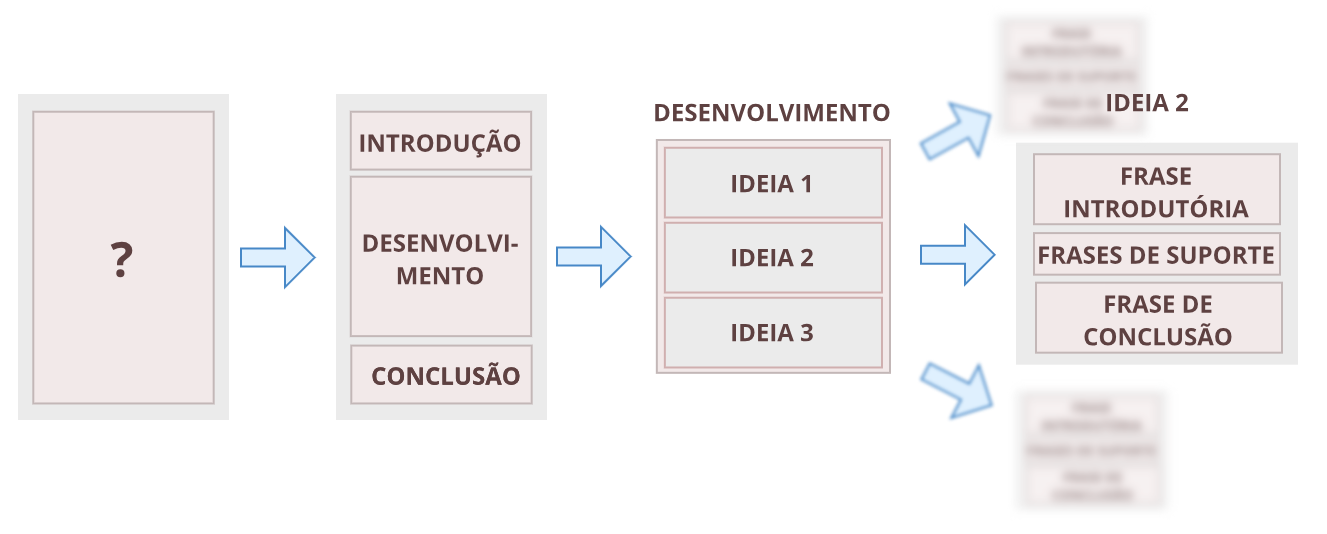
\includegraphics[width=1\linewidth]{figs/decomposition.png}    
            \end{center}
            
            \\ \hline
            
            \textbf{Reconhecimento de Padrões}: Identificar similaridades entre as partes de um problema para resolvê-las com eficiência \cite{bbc_learning_what_2015}. Na Ciência da Computação os padrões reduzem a complexidade por meio da generalização de soluções para aplicá-las em múltiplas situações \cite{k-12_computer_science_framework_k12_2016}.
            &
            Um exemplo é reconhecer padrões em sequências de cores. A primeira vista são apenas círculos coloridos, mas é possível identificar o padrão sequencial de cores em cada linha. Outros exemplos são identificar rotas comuns entre casa e trabalho para organizar caronas, identificar o padrão de compras no mercado para dispor produtos, e também reconhecer sintomas similares de doenças entre pacientes.
            &
            \begin{center}
                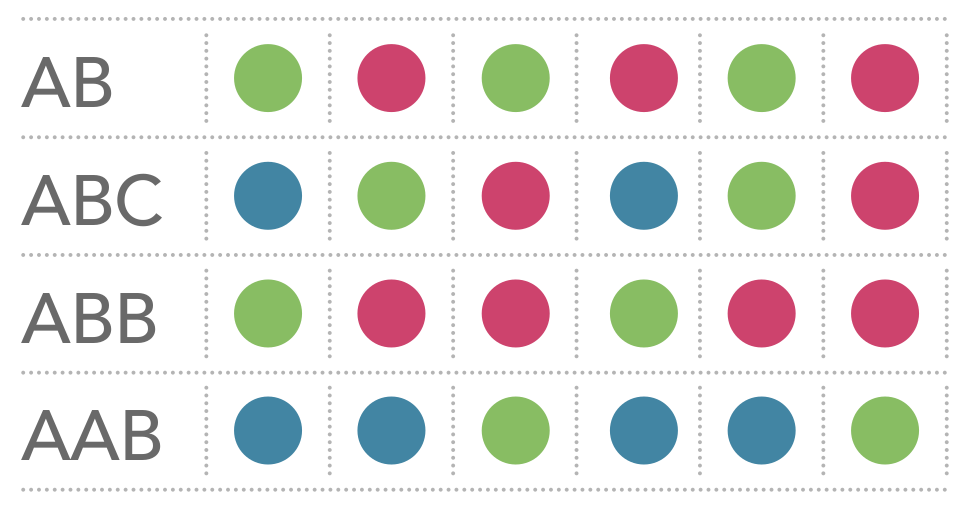
\includegraphics[width=1\linewidth]{figs/pattern_recognition.png}    
            \end{center}
            \\ \hline
            \textbf{Abstração}: Destacar detalhes importantes e ignorar detalhes desnecessários \cite{wing_computational_2008}. A abstração elimina os detalhes específicos, inúteis para resolver um problema, e cria uma ideia base da solução denominada modelo \cite{bbc_learning_what_2015}.
            &
            Durante o treinamento de cães farejadores para resgate de seres humanos, um conjunto de testes avalia os animais em quesitos como inteligência, concentração, agilidade e capacidade olfativa. Dados como raça, tamanho, cor ou peso não influenciam na capacidade do cão desempenhar a tarefa em questão. É preciso, portanto, detectar as características relevantes ao problema no universo de características do animal \cite{davidson_12_2018}.
            &
            \begin{center}
                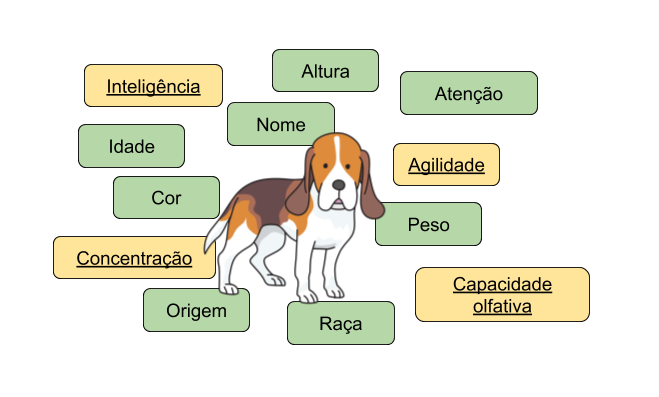
\includegraphics[width=1\linewidth]{figs/abstraction.png}    
            \end{center}
            
            \\ \hline
            \textbf{Algoritmos}: instruções que demonstram o passo a passo para resolver um problema. Esse conjunto de passos precisa ter um início, um fim, e uma sequência de instruções sem ambiguidade \cite{bbc_learning_what_2015}.
            
            &
            A representação desse conjunto de passos pode ocorrer por diferentes modos. Uma receita de bolo é um algoritmo, pois define o conjunto de passos para resolver o problema de criar um bolo. Neste caso a representação é textual, porém pode-se representar um algoritmo por fluxogramas, blocos, sequência de símbolos, etc.
            &
            \begin{center}
                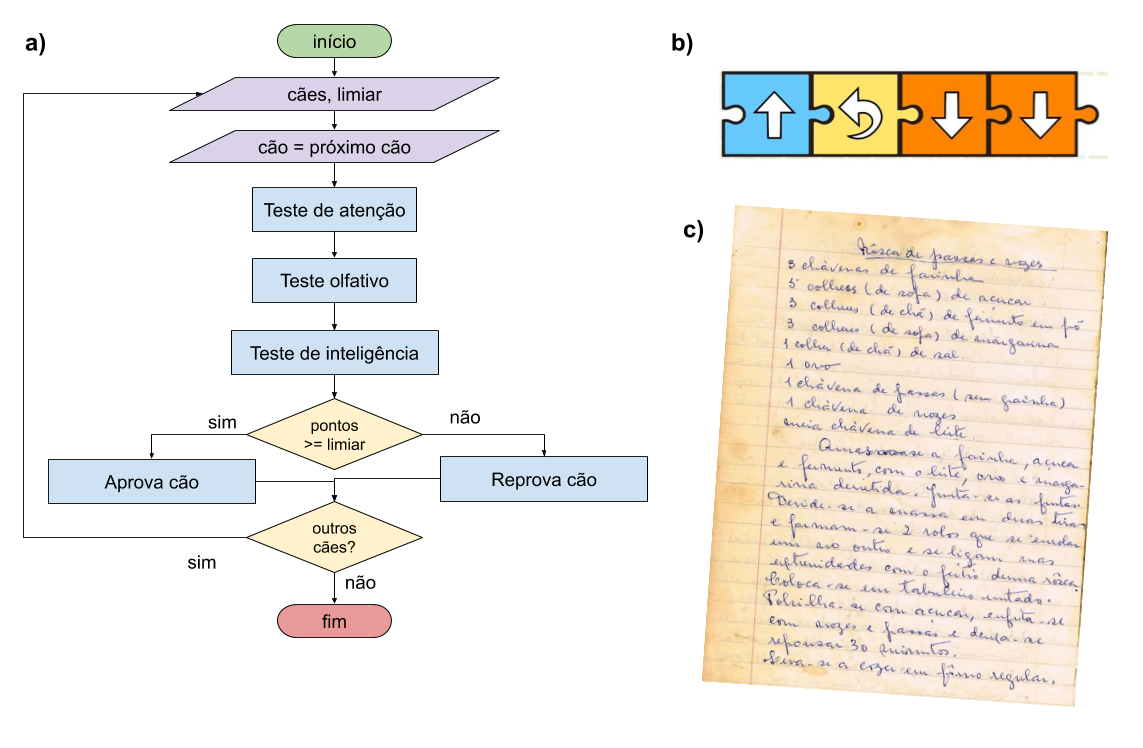
\includegraphics[width=1\linewidth]{figs/algoritmo.png}    
            \end{center}
            
            \\ \hline
            
        \end{tabular}
         
        \end{footnotesize}
    \end{center}
    \end{quadro}
\end{landscape}

As definições de PC apresentadas estão relacionadas com resolução de problemas de modo geral, e não se restringem ao contexto da programação de algoritmos. Nessas definições, o conceito de depuração parece ter relevância secundária, sendo pouco citado. Uma possível causa é o fato da depuração estar "embutida" na prática de programar algoritmos, e não ser percebida como uma habilidade útil no dia a dia. \citeonline{mccauley_debugging_2008} comenta que até mesmo no campo da programação a depuração é negligenciada, afirmando que o livro de Barnes e Kölling (2002) é um dos poucos a dedicar um capítulo completo sobre depuração. A próxima seção busca esclarecer este conceito.

\subsection{Depuração}

A depuração é um conceito que foi particularmente discutido por pesquisadores e educadores nas décadas de 1970 \cite{mccauley_debugging_2008} e 1980 \cite{sipitakiat_robo-blocks_2012}. Mesmo já sendo praticada por programadores profissionais, foi o surgimento da linguagem Logo neste período que desencadeou estudos envolvendo depuração por crianças. A recente popularização do PC \cite{ilic_publication_2018} e o aumento do contato de crianças com algoritmos tem levado pesquisadores a discutirem o papel da depuração no aprendizado \cite{repiso_robotics_2019}.

A atividade de depurar está ligada à necessidade de corrigir partes de algoritmos que impedem a execução correta de um programa. No contexto educacional, este desejo cria uma situação propícia ao exercício de um conjunto maior de habilidades, como trabalho em equipe, comunicação e persistência \cite{sipitakiat_robo-blocks_2012}. Portanto, pode ser vista como uma atividade de resolver problemas, que envolve observar, comunicar e refletir. A depuração, bem como a ação de ler e acompanhar a execução passo a passo de programas existentes, são consideradas essenciais para aprender programação \cite{mccauley_debugging_2008} e contribuir para o desenvolvimento do \ac{PC}.

Entretanto, \citeonline{liu_understanding_2017} observam que a depuração é um componente do PC negligenciado principalmente nos níveis iniciais de ensino. Os avanços tecnológicos e o entusiasmo com a temática do PC tem levado estudantes iniciarem o aprendizado de programação mais jovens. Ainda assim, afirma que poucos ambientes de programação são projetados com foco em funcionalidades de depuração no nível da Educação Básica, e a maior parte das pesquisas sobre o tema ocorrem com estudantes em nível universitário.

\citeonline{brennan_new_2012} abordam a depuração em um framework de PC utilizado no contexto do ScratchJr. O framework tem três dimensões: conceitos, práticas e perspectivas. Os conceitos remetem aos conhecimentos utilizados e aprendidos durante a programação, como paralelismo, laços de repetição e dados. As práticas envolvem a aplicação desses conceitos utilizando de desenvolvimento iterativo, mesclagem de códigos e depuração. Por fim, as perspectivas são formas de se utilizar a tecnologia: como meio de expressão, conexão, e questionamento/mudança da realidade. Usando esse framework, \citeonline{lye_review_2014} revisaram a literatura em busca de trabalhos sobre PC. Eles observam que 85\% dos artigos analisaram os aprendizados de PC relacionados a conceitos, e apenas 22\% analisaram as práticas. Argumentam que por isso seria necessário mais trabalhos ligados à praticas computacionais como a depuração.

\citeonline{wong_computational_2018} relacionam pensamento algorítimico e depuração como duas sub-habilidades do PC. O pensamento algorítmico seria a capacidade de formular sequências de passos para solucionar um problema independente de computador. A depuração seria aplicada depois do pensamento algorítmico, ao traduzir o algoritmo para um programa de computador e solucionar problemas no código do programa se este não gerar o resultado desejado. Papert, por outro lado, afirma que a depuração independe do computador, pois "estratégias de depuração foram desenvolvidas por estudantes de sucesso muito antes da existência dos computadores" \cite[p.23]{papert_mindstorms:_1980}. Seria, então, mais um processo mental do que o uso de ferramentas computacionais.

\citeonline{carver_assessing_1986} decompõem o processo da depuração em quatro etapas: (i) avaliar o programa, (ii) identificar o \bug, (iii) localizar o \bug, (iv) e corrigir o \bug. Em uma atividade com BPs, por exemplo (ver \autoref{fig_ex_carver_klar}), a criança executa o algoritmo e verifica se alcançou o resultado esperado. Caso contrário, precisa identificar o erro, por exemplo, se o brinquedo está no local errado, se virou para o lado errado, etc. Ainda na identificação, constrói hipóteses causas do problema. Faltou adicionar um comando de giro? O comando de giro está errado? A terceira etapa passa a ter contato com o código, onde a criança identifica qual peça pode ser o \bug. Por fim, na última etapa a criança modifica o programa, adicionando ou removendo a peça apontada na etapa 3 e o ciclo recomeça com uma nova execução.

\begin{figure}[!htpb]
  \centering
  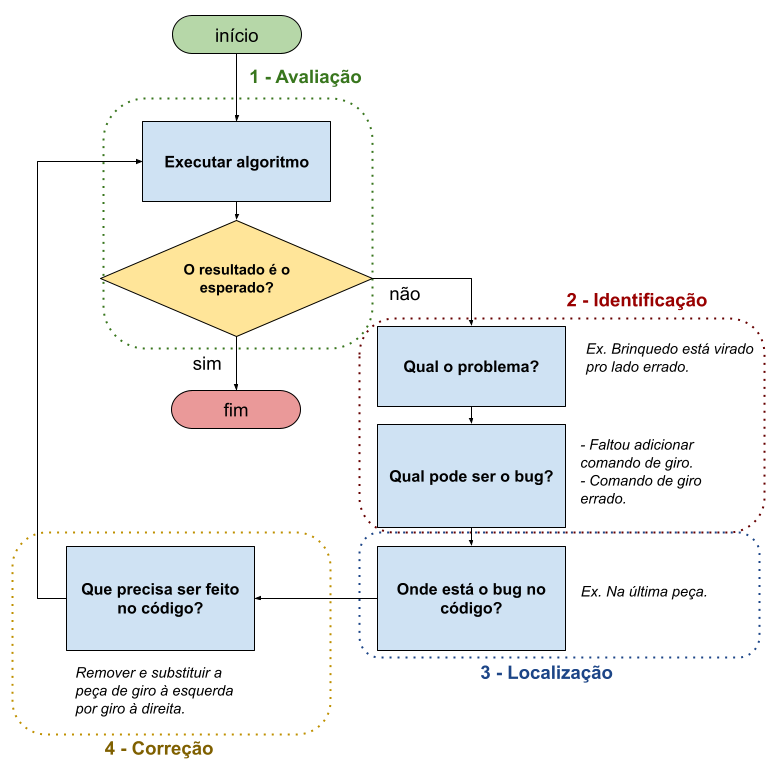
\includegraphics[width=.8\linewidth,fbox]{figs/ex_depuracao_carver_klar.png}
  \caption{Processo de depuração proposto por \citeonline{carver_assessing_1986} no contexto de um BP. }
  \sourceauthor
  \label{fig_ex_carver_klar}
\end{figure}

Seguindo esse modelo, \citeonline{carver_assessing_1986} avaliaram o aprendizado de depuração por crianças entre 7 e 8 anos. As crianças trabalharam em pares durante 22 horas de curso sobre a linguagem Logo. Os pesquisadores aplicaram 3 testes, sendo dois em dupla e um individual. Os testes avaliaram habilidade de depuração, interpretação de código, escrita de código e uso do ambiente Logo. Os resultados indicaram que as crianças depuraram somente quando lhes era solicitado, e que a estratégia utilizada para encontrar erros foi procurar linha por linha, sem uma estratégia eficiente. Os pesquisadores também perceberam que as crianças preferiram apagar o programa em vez de depurar. Por fim, concluem que depurar é uma atividade complexa, pouco ensinada, e que exige memória de trabalho para observar o programa criado e os problemas existentes. Além disso, menciona que o fato do erro ser punido pelo sistema educacional leva a criança a tentar eliminá-lo (apagar todo o programa) em vez de resolvê-lo.

\subsection{Depuração e visibilidade}
Em uma revisão sistemática, \citeonline{mccauley_debugging_2008} apresenta modelos de depuração definidos Vessey (1985) e Katz e Anderson (1987). Vessey (1985) define depuração em cinco passos: (i) determinar o problema comparando o resultado errado e o correto; (ii) \textit{obter familiaridade com a estrutura do programa}; (iii) explorar a execução do programa; (iv) levantar hipóteses para a causa do erro; e (v) reparar o erro. Katz e Anderson (1987) definem quatro passos: (i) entender o sistema, (ii) testar o sistema, (iii) \textit{localizar o erro}, e (iv) reparar o erro.

\begin{figure}[!htpb]
  \centering
  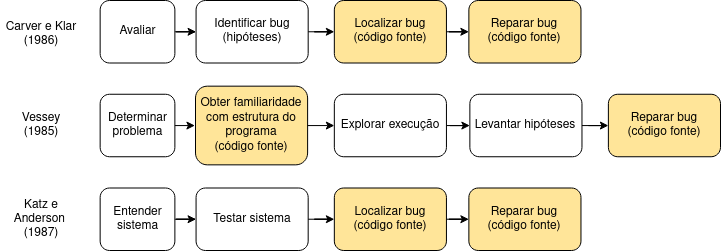
\includegraphics[width=.9\linewidth,fbox]{figs/debug_models.png}
  \caption{Modelos de depuração.}
  \sourceauthor
  \label{fig_debug_models}
\end{figure}

Estes modelos têm em comum um passo de observar a estrutura do algoritmo para localizar o erro (destacados na \autoref{fig_debug_models}). A localização do erro presume que um código fonte possa ser visto e analisado. Essa necessidade está ligada ao que \citeonline{norman_design_1988} apresenta como um dos princípios mais importantes do design: a visibilidade. Esse princípio permite o “mapeamento entre as ações pretendidas e as ações concretas” \cite{norman_design_1988}. Para isso, as ações possíveis de se realizar com uma interface devem estar visíveis e seus efeitos devem ser óbvios e imediatos.

Interfaces de programação que não atendem o princípio da visibilidade tornam difícil a atividade de depurar algoritmos. Este problema aparece em ferramentas projetadas para crianças, como a Bee-Bot. A interface deste brinquedo apresenta botões de direção e um botão de limpeza de memória, que apaga os comandos direcionais do brinquedo. A falta de visibilidade se dá na ausência de um \textit{display} para mostrar os comandos presentes na memória do brinquedo. Ao não ver os comandos que estão programados, as crianças esquecem de limpar a memória do brinquedo e então pensam estar criando um novo programa \cite{raabe_brinquedos_2015}. A falta de visibilidade impede perceber que na verdade os comandos inseridos anteriormente ainda estão presentes, e os novos comandos estão sendo adicionados no final da sequência, criando um programa cada vez maior.

Durante este processo ocorre um fenômeno mencionado por \citeonline{norman_design_1988} como a formação do \destaque{modelo mental} do usuário. O modelo mental é a compreensão que o usuário tem de como se comunicar com um dispositivo, sistema, etc, a fim de obter determinado resultado. Para formar o modelo mental é essencial que o usuário perceba o estado atual do dispositivo, por meio da visibilidade. Quando a interface com o dispositivo não é clara ou a apresentação do estado atual é ambíguo, o comportamento do dispositivo pode não se adequar ao modelo mental idealizado pelo usuário.

A questão é que, quando o inesperado acontece, o cérebro humano tenta explicar e acomodar essa nova situação a um entendimento prévio. No caso da Bee-Bot, ao ver o brinquedo executar movimentos diferentes dos últimos comandos programados - que ocorre pela diferença entre o modelo pensado pela criança e o estado real do brinquedo - as crianças tendem a explicar que o brinquedo está "tomando suas próprias decisões". Neste instante a criança adapta o seu modelo mental, a fim de explicar o comportamento inesperado do dispositivo computacional, quando este não executa a sequência de passos que a criança imaginou que ele executaria.

Uma alternativa para interfaces com o problema de falta de visibilidade são os ambientes de programação em blocos (\autoref{sec_prog_blocos}). \citeonline{wong_computational_2018} atribuem a melhoria na habilidade de depuração de crianças do 5º ano do Ensino Fundamental às "características de visualização da programação em blocos, pois os efeitos do programa podem ser vistos diretamente". \citeonline{bers_coding_2019} falam sobre as vantagens de visualização das interfaces de programação em blocos, neste caso blocos tangíveis:

\begin{citacao}
As crianças podem ver o que não funciona e podem ajudar a consertar. [...] A visibilidade adicional do código pode chamar a atenção para propriedades e conceitos anteriormente negligenciados, como elegância, a importância da depuração e teste para casos extremos e outras situações incomuns. Em outras palavras, o código tem o potencial de se tornar um objeto de conversa e atenção de uma forma que não poderia ser antes. \cite[p.14, tradução nossa]{bers_coding_2019}
\end{citacao}

Além de promover a visibilidade, a programação em blocos evita problemas de interação presentes em outros tipos de interface, como a programação textual.
Esta, apesar de também mostrar os comandos, não é acessível para crianças devido a erros de sintaxe e à necessidade de lembrar o que é preciso digitar. Os blocos, por outro lado, estão sempre disponíveis, geralmente agrupados por similaridade, de modo que não seja necessário lembrar sequências de caracteres para digitar num teclado. Além disso, o formato dos encaixes sugere como relacionar os blocos de modo coerente.

A visibilidade da programação em blocos também favorece a interação social, tornando o código um objeto de conversa. O mesmo ocorre com a depuração, que é uma atividade estabelecida socialmente por meio de falas, apontamentos e olhares, e neste sentido os artefatos têm papel central \cite{heikkila_debugging_2018}. Esta ligação entre blocos e depuração favorece o princípio da linguagem Logo, de permitir depurar o que se passa na mente da criança \cite{solomon_history_2020}. Por meio de artefatos compartilhados socialmente, um adulto pode entender melhor o algoritmo que a criança tenta expressar. Assim, consegue auxiliá-la a desenvolver seu modelo mental de como construir um algoritmo para produzir um resultado desejado.

\section{Interfaces de Programação para Crianças}
\label{section_interfaces}

Aprender algoritmos parece ser uma tarefa difícil, mesmo para adultos. Analisando cursos de graduação em Computação de universidades dos Estados Unidos, Israel, Polônia e Austrália, \citeonline{mccracken_multi-national_2001} concluíram que os estudantes não possuíam as habilidades de programação esperada pelos professores, indicando dificuldade no aprendizado de algoritmos. \citeonline{hoed_alise_2016} cita a reprovação na disciplina de Algoritmos entre as causas de evasão em cursos de Computação.

Felizmente, pesquisas sugerem que crianças podem aprender noções de algoritmos. \citeonline{sheehan_parent-child_2019}, observaram 31 crianças de 4.5 a 5 anos de idade, durante a interação com um aplicativo de programação. Os autores concluem que as crianças conseguiram produzir e compreender algoritmos básicos para definir o comportamento de um personagem. Em outro estudo, com 53 crianças de 4 a 6 anos, \citeonline{bers_computational_2014} identificam que 75\% das mesmas selecionaram e sequenciaram corretamente as instruções ao programar um veículo robótico.

Os benefícios de aprender algoritmos transcendem os campos estritamente tecnológicos. Conforme lembram \citeonline{ciftci_effect_2020}, os algoritmos possuem conceitos que se intersectam com os da matemática, como variáveis, laços de repetição e condicionais. Esses autores também afirmam que programar pode auxiliar estudantes a analisarem seu modo de raciocínio, reorganizar tarefas seguindo um processo de resolução de problemas e desenvolver habilidades não-verbais. Em experimento, os autores verificaram um aumento significativo dessas habilidades em crianças de 4 a 5 anos que participaram de um curso de programação durante 8 semanas.

Para \citeonline{papert_mindstorms:_1980},

\begin{citacao}
Quando a criança aprende a programar, o processo de aprendizado é transformado. Ele se torna mais ativo e autodirigido. Em particular, o conhecimento é adquirido para um propósito pessoal reconhecido. A criança faz algo com ele. O novo conhecimento é uma fonte de poder e é experimentado como tal desde o momento em que começa a tomar forma na mente da criança \cite[p.21, tradução nossa]{papert_exploration_1996}.
\end{citacao}

Uma das primeiras experiências envolvendo crianças e programação é atribuída a Papert e Cynthia Solomon em 1968. Ambos foram até uma escola de um subúrbio de Boston ensinar programação para jovens. O computador que executou os programas estava em um laboratório a alguns quilômetros de distância. Por esse motivo, as crianças interagiram usando terminais, nos quais digitaram comandos na linguagem LOGO.

Conforme novas versões da linguagem eram desenvolvidas, pesquisadores iam até as escolas para ensinar e observar o uso da linguagem em sala de aula \cite{bers_coding_2018}. Solomon destaca o papel da participação das crianças durante o desenvolvimento da linguagem, dando \textit{feedback} e influenciando diversas questões de design:

\begin{citacao}
O trabalho iniciou o que se tornou uma linguagem poderosa, flexível e usável para crianças e destacou a facilidade com que os aprendizes adquiriram expertise sobre a ferramenta. O trabalho é também um importante exemplo de envolvimento das crianças no design de uma nova tecnologia e de como a tecnologia pode se beneficiar da expertise e do \textit{feedback} das crianças. Cada vez que Seymour e eu trabalhamos com as crianças, LOGO foi radicalmente redesenhada incorporando o seu \textit{feedback}.
\end{citacao}

A linguagem LOGO inicialmente permitia manipular palavras, e deste modo as crianças construíam poemas e geradores de frases. Papert, um matemático, percebeu a necessidade transcender o campo das palavras e de permitir às crianças brincarem com formas, ângulos e desenhos. Dessa percepção nasceu a ideia de uma tartaruga capaz de se mover e desenhar figuras geométricas. Essa tartaruga foi introduzida primeiro virtualmente, mas depois tomou formas físicas e originando os primeiros brinquedos programáveis.

\subsection{Brinquedos Programáveis}
\label{brinquedos_programaveis}
Brinquedos programáveis são robôs cuja função é possibilitar a crianças o contato com conceitos matemáticos e algoritmos. O que os diferencia das outras ferramentas de programação é a aparência lúdica, que reflete o imaginário do público infantil \cite{raabe_2017_rope}. Pesquisas mencionam que os brinquedos programáveis podem promover habilidades relacionadas do \ac{PC} \cite{repiso_robotics_2019, bers_coding_2018, pugnali_impact_2017,  bers_computational_2014}, como pensamento algorítmico, reconhecimento de padrões, abstração e decomposição.

A interface intuitiva é o que permite que crianças possam programar esses brinquedos. A busca por interfaces intuitivas ocorre desde a linguagem LOGO, e com o desenvolvimento das tecnologias de hardware a diversas alternativas de interação têm surgido nos últimos anos \cite{catlin_edurobots_2018}. Por isso, pesquisas têm buscado classificar essas interfaces.

\citeonline{hamilton_emerging_2020} apresentam 30 brinquedos e os classificam segundo suas características físicas em seis categorias: (i) jogos de tabuleiro ou livros; (ii) eletrônicos não robóticos; (iii) robôs controlados por tela; (iv) robôs operados por botões; (v) robôs com interface tangível; e (vi) híbridos \autoref{hamilton}.

\begin{figure}[!htpb]
  \centering
  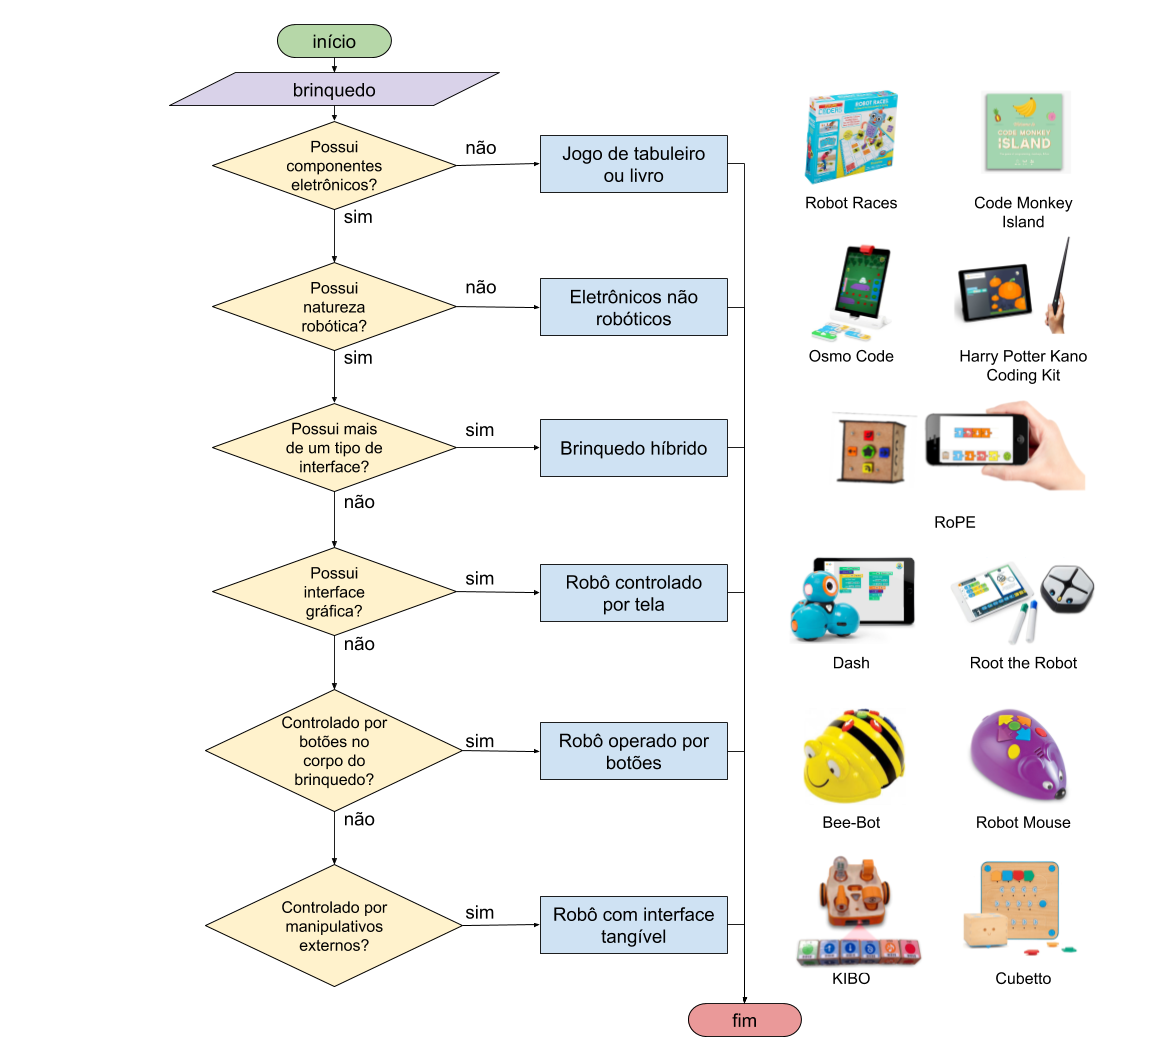
\includegraphics[width=.9\linewidth,fbox]{figs/hamilton_classification.png}
  \caption{Classificação de brinquedos programáveis por características físicas.}
  \source{ Adaptado de \citeonline{hamilton_emerging_2020}.}
  \label{hamilton}
\end{figure}

Em outra revisão, \citeonline{yu_review_2019} também analisam um conjunto de 30 brinquedos programáveis e kits de robótica focados em crianças de até 7 anos. A análise ocorre sob as perspectivas de design, \acl{PC}, expressividade e suporte a domínios\footnote{
A expressividade corresponde à variedade de atividades possibilitadas pelo kit, e o suporte a domínios se refere ao conjunto de assuntos/conteúdos passíveis de serem apresentados no contexto dessas atividades.
}.

Quanto ao design, \citeonline{yu_review_2019} distinguem três categorias de kits: físicos, virtuais e híbridos. As três categorias têm o comum a utilização de blocos de código relacionados a movimentos, com cada bloco tendo uma cor diferente para auxiliar na distinção dos diferentes
comandos. Esses blocos comumente tem o formato de peças de quebra-cabeça. Os kits físicos, como KIBO e Cubetto, possuem todos os componentes tangíveis, geralmente incluindo um robô com rodas, um conjunto de blocos de código e materiais de suporte como mapas, livros e materiais de personalização. Alguns robôs são controlados por botões, mas a maioria tem blocos de códigos separados.

Os kits virtuais são aqueles que não possuem parte tangível. Exemplos são aplicativos de \textit{smartfone} e jogos de computador, que possibilitam construir cenas, programar personagens e resolver problemas ao arrastar e soltar blocos de código virtuais. O Scratch e o ScrachJr são exemplos de aplicativos que permitem construir cenas e programar personagens. Essa categoria remete às primeiras experiências de Papert durante o desenvolvimento da linguagem LOGO, que permitia definir o comportamento da tartaruga virtual. A diferença é que as ferramentas atuais priorizam o uso de linguagens de blocos para evitar erros de sintaxe.

A terceira categoria são os kits híbridos, onde há união de partes tangíveis e virtuais. \citeonline{yu_review_2019} destacam que há dois tipos de kits híbridos: aqueles com blocos físicos que controlam personagens virtuais (brinquedos da empresa Osmo, por exemplo\footnote{\url{https://www.playosmo.com/en/coding/}}), e aqueles que possuem blocos virtuais para controlar personagens físicos.

Quanto ao \acl{PC}, \citeonline{yu_review_2019} relacionam atividades possibilitadas pelos BPs e kits capazes de promover os conceitos e práticas ligadas ao \ac{PC} definidas por \citeonline{brennan_new_2012}. Os autores identificam que as atividades com BPs podem abordar todos os conceitos e práticas do \ac{PC}. Há poucos kits, porém, que suportam as práticas de reutilização/combinação e abstração/modularização.

\begin{quadro}[!htbp]
 \captionquadro{Como brinquedos programáveis e kits promovem conceitos e práticas computacionais.}
 \label{quadro_brinquedos_praticas}
 \begin{center}
 \begin{footnotesize}
\begin{tabular}{|p{3cm}|p{12cm}|}
\hline
\multicolumn{2}{|c|}{\textbf{Conceitos}} \\ \hline

    Sequenciamento & Criar uma sequência de código para programar o movimento ou outros efeitos em robôs físicos ou virtuais. \\ \hline
    
    Repetições & Encapsular uma sequência de comandos em blocos de repetição para executar repetidas vezes. \\ \hline
    
    Eventos & Executar ações ao apertar botões específicos, ou programar efeitos durante interações entre brinquedos (por exemplo, Dash e Dot executam ações quando se aproximam um do outro). \\ \hline
    
    Paralelismo & Controlar o movimento de diversos robôs/sprites simultaneamente, ou programar efeitos simultâneos de movimento, luzes e sons. \\ \hline
    
    Condicionais & Programar ações dependentes de eventos disparados por sensores ou mapas. \\ \hline
    
    Operadores & Possibilitar realizar operações matemáticas simples. \\ \hline
    
    Dados & Ajustar parâmetros como distância do movimento, rotação, etc. \\ \hline

\multicolumn{2}{|c|}{\textbf{Práticas}} \\ \hline

    Desenvolvimento iterativo e incremental & Permitir erros e tentativas ilimitados. Constantemente revisar e adicionar novos blocos de código (ex. ScratchJr). \\ \hline
    
    Teste e depuração & Testar continuamente o código durante o desenvolvimento e depurar se algo não funciona. \\ \hline
    
    Reutilização e combinação & Construir projetos partindo de projetos anteriores (ex. Scratch). A maioria dos kits não suporta essa prática. \\ \hline
    
    Abstração e modularização & Construir blocos de código que podem ser chamados de outros locais (ex. Cubetto). Poucos kits suportam essa prática. \\ \hline

\end{tabular}
 
 \end{footnotesize}
 \end{center}
 \source{Adaptado de \citeonline{yu_review_2019}.}
\end{quadro}

Quanto à expressividade, ou seja, as atividades que os brinquedos possibilitam, os autores citam três principais modalidades. A primeira corresponde a mover o brinquedo/kit por um caminho ou sobre um mapa para coletar objetos. A segunda modalidade é a contação de histórias: os brinquedos se movem sobre cenários, e as crianças podem criar histórias para os mesmos em conjunto com a família. Há também um terceiro tipo de atividade: decorar e personalizar a aparência do brinquedo.

Quanto ao suporte a domínios, \citeonline{yu_review_2019} mencionam o desenvolvimento de narrativas, conceitos matemáticos e conceitos de engenharia. O desenvolvimento de narrativas está ligado às atividades de contação de histórias. O Scratch, por exemplo, possibilita criar narrativas por meio da programação de personagens e definição de cenários. Conceitos matemáticos aparecem ao definir distâncias de movimentos, e operações aritméticas simples também estão presentes em alguns brinquedos. Os conceitos de engenharia são abordados em brinquedos onde é possível unir partes diversas e observar efeitos, como o caso do Cubelets\footnote{\url{https://www.modrobotics.com/\#whatr-cubelets}}, que permite à criança unir cubos de luminosidade, sensores e movimentos.

As classificações de \citeonline{hamilton_emerging_2020} e de \citeonline{yu_review_2019} se diferem quanto aos critérios utilizados. Enquanto \citeonline{hamilton_emerging_2020} não inclui em sua lista os kits robóticos e softwares exclusivamente gráficos, \citeonline{yu_review_2019} inclui ambos. Ambos os trabalhos, porém, focam no público infantil, e as análises das interfaces e dos conceitos promovidos são úteis para definir as características do brinquedo RoPE.

\subsubsection{RoPE - Robô Programável Educacional}
O RoPE é um brinquedo programável desenvolvido para crianças a partir de 3 anos, que busca estimular o \acl{PC} e a criatividade. Ele permite à criança inserir comandos que ele então executa em forma de movimentos sobre um tapete temático. A construção tem preocupações de design relacionadas às crianças e ao ambiente. Quanto às crianças, o tamanho dos botões leva em conta que a coordenação motora ainda está em desenvolvimento. Quanto ao ambiente, as cores dos botões facilitam a comunicação das professoras para indicarem um botão específico durante alguma explicação.

\begin{figure}[!htpb]
  \centering
  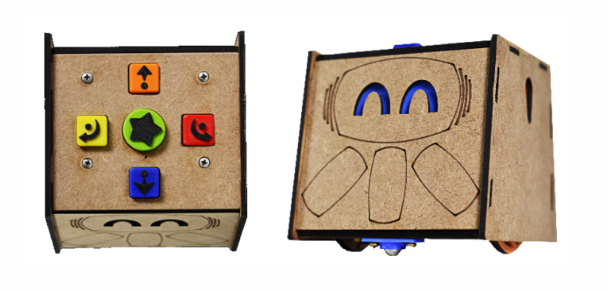
\includegraphics[width=.9\linewidth,fbox]{figs/rope_up_front.png}
  \caption{Visão superior e frontal do RoPE.}
  \source{Smartfun Brasil.}
  \label{rope}
\end{figure}
O RoPE pode ser operado de duas formas: botões na parte superior e um aplicativo de \textit{smartphone}. A primeira interface é formada por 5 botões que fazem parte do brinquedo. Seus comandos são (1) girar para esquerda 90 graus, (2) girar para direita 90 graus, (3) movimentar para frente (4) movimentar para trás, e (5) executar instruções da memória ou limpar memória. A execução de cada instrução provoca, além do movimento, a emissão de um som característico e uma luz da mesma cor do botão gerador da instrução, de forma a haver uma tríade cor-movimento-som. Um som de finalização indica quando o brinquedo executou todas as instruções \cite{raabe_2017_rope}.

A segunda interface é um aplicativo de celular que permite programar o RoPE a distância (\autoref{rope_app}). O programa aparece na tela em formato de peças de quebra-cabeça conectadas. A comunicação Bluetooth entre o brinquedo e o aplicativo possibilita manter as peças e as instruções da memória em sincronia. A reordenação das peças no aplicativo é replicada no brinquedo e o pressionamento de um botão do brinquedo é replicado nas peças na tela do celular. Considerando, então, a possibilidade de programar por meio de duas interfaces, as classificações de \citeonline{hamilton_emerging_2020} e \citeonline{yu_review_2019} posicionam o RoPE como um brinquedo híbrido.

\begin{figure}[!htpb]
  \centering
  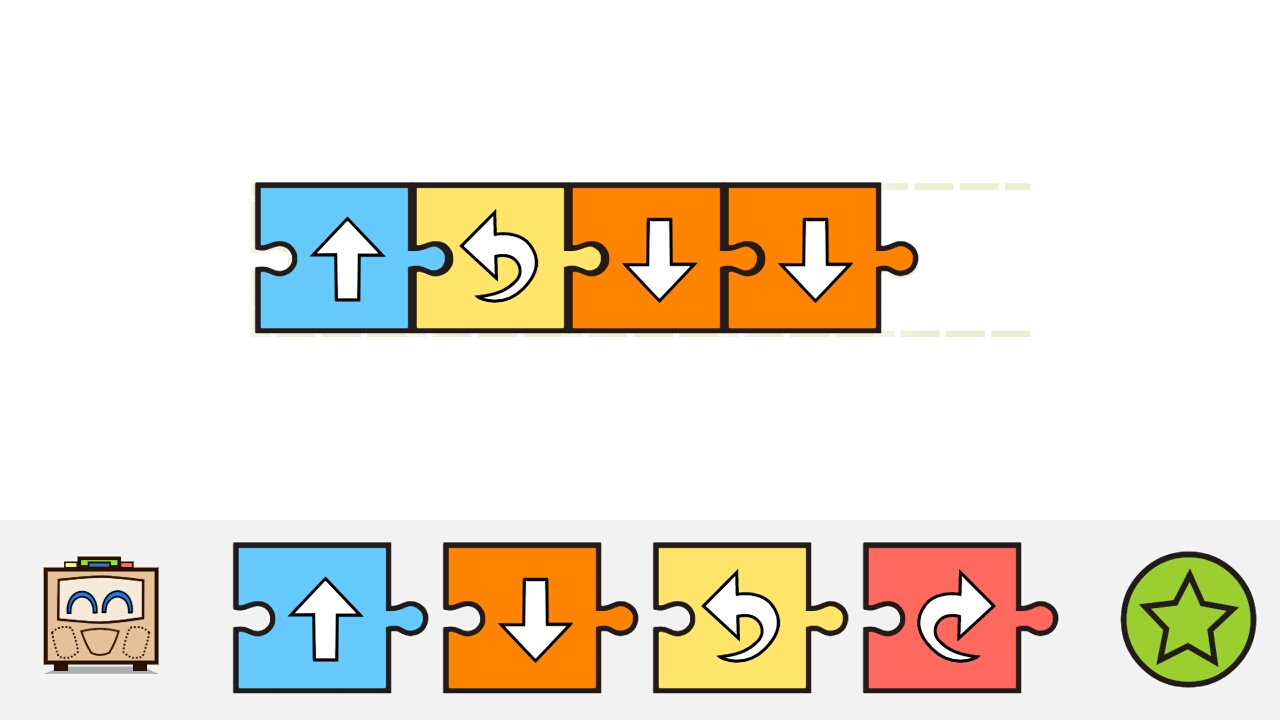
\includegraphics[width=.9\linewidth,fbox]{figs/app.jpg}
  \caption{Aplicativo para programar o RoPE.}
  \sourceauthor
  \label{rope_app}
\end{figure}

O \autoref{quadro_rope_pc} classifica o RoPE quanto aos aspectos do \acl{PC}. Os conceitos abordados pelo brinquedo são sequenciamento, eventos e dados. O brinquedo aborda diretamente apenas sequenciamento e eventos, porém as professoras podem abordar o conceito de dados durante o uso do brinquedo, ao definir distâncias e posições a serem alcançadas. O brinquedo não abrange todas as práticas e conceitos pois o público-alvo são crianças da Educação Infantil e é preciso manter um design simplificado.

\begin{quadro}[!htbp]
 \captionquadro{Conceitos e práticas computacionais e sua promoção pelo brinquedo RoPE.}
 \label{quadro_rope_pc}
 \begin{center}
 \begin{footnotesize}
\begin{tabular}{|p{5cm}|p{10cm}|}
\hline
\multicolumn{2}{|c|}{\textbf{Conceitos}} \\ \hline
    
    Sequenciamento & Criar uma sequência de comandos para guiar o movimento do RoPE sobre um mapa. \\ \hline
    
    Repetições & \notcovered \\ \hline
    
    Eventos & O evento de clicar na estrela inicia a execução dos comandos inseridos previamente. \\ \hline
    
    Paralelismo & \notcovered \\ \hline
    
    Condicionais & \notcovered \\ \hline
    
    Operadores & \notcovered \\ \hline
    
    Dados & Estimar o número de passos para alcançar uma posição no mapa. \\ \hline

\multicolumn{2}{|c|}{\textbf{Práticas}} \\ \hline

    Desenvolvimento iterativo e incremental & Não abordado diretamente, pois as instruções são apagadas do brinquedo ao final de cada execução. \\ \hline
    
    Teste e depuração & Testar continuamente o código durante o desenvolvimento e depurar se algo não funciona. \\ \hline
    
    Reutilização e combinação & \notcovered \\ \hline
    
    Abstração e modularização & \notcovered \\ \hline

\end{tabular}
 
 \end{footnotesize}
 \end{center}
 \sourceauthor
\end{quadro}

Além de aspectos ligados ao PC, o RoPE suporta domínios multidisciplinares por meio de tapetes temáticos, nos quais as crianças têm contato com letras do alfabeto (\autoref{tapete_alfabeto}), temáticas dos ambientes rurais (\autoref{tapete_farm}) e urbanos (\autoref{tapete_city}). \citeonline{pinheiro_alise_2016} desenvolveu um software que permite à criança gerar seus próprios mapas e percebeu mais engajamento das crianças ao usarem seus próprios mapas. Esses tapetes também podem ser criados manualmente, como o tapete criado pelas crianças da \autoref{tapete_alfabeto}. Além de criar os próprios tapetes \citeonline{martins_desenvolvimento_2016} também menciona a possibilidade de customizar a carcaça do brinquedo. Então, apesar de a interface do brinquedo favorecer raciocínio matemático de estimar quantidades e movimentos, a customização e os tapetes possibilitam criar micromundos infinitos associados a qualquer temática.

\begin{figure}[!htbp]
    \centering
    \begin{subfigure}{.33\textwidth}
        \centering
        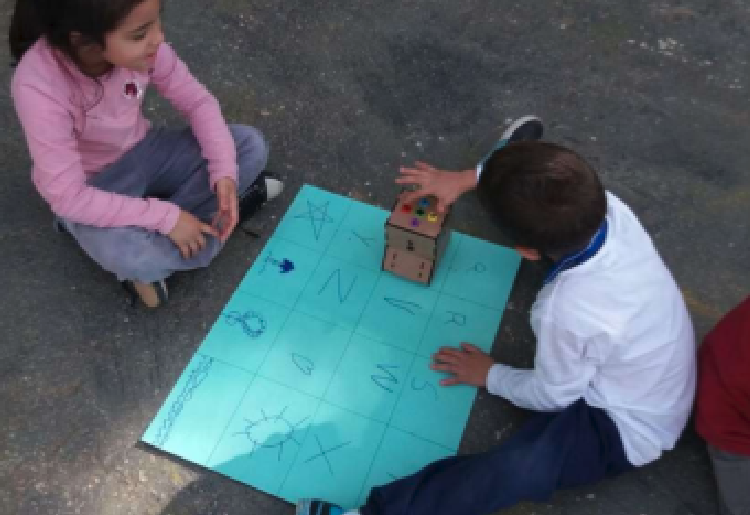
\includegraphics[width=.9\linewidth,fbox]{figs/tapete_alfabeto.png}
        \caption{Letras do alfabeto}
        \label{tapete_alfabeto}
    \end{subfigure}%
    \begin{subfigure}{.33\textwidth}
        \centering
        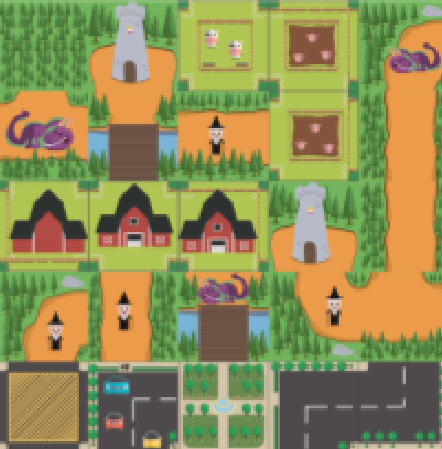
\includegraphics[width=.9\linewidth,fbox]{figs/tapete_farm.png}
        \caption{Ambiente rural}
        \label{tapete_farm}
    \end{subfigure}
    \begin{subfigure}{.33\textwidth}
        \centering
        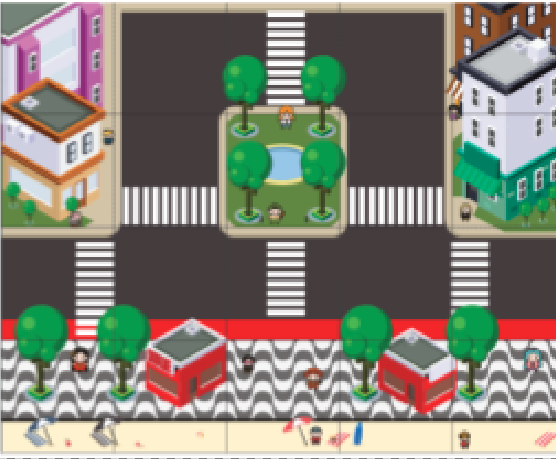
\includegraphics[width=.9\linewidth,fbox]{figs/tapete_city.png}
        \caption{Ambiente urbano}
        \label{tapete_city}
    \end{subfigure}
    \caption{Tapetes temáticos.}
    \sourceauthor
    \label{rope_mats}
\end{figure}

\subsection{Interfaces Tangíveis}
\label{fundamentacao_sub_interfaces_tangiveis}
Como abordado na \autoref{brinquedos_programaveis}, as interfaces tangíveis representam um dos tipos de interfaces utilizadas pelos brinquedos de programar. O conceito de interfaces tangíveis, entretanto, é amplo e tem fronteiras difusas \cite{falcao_design_2007}. A ideia inicial sobre tangibilidade é que apresenta formas físicas de interação, que permitem o contato da mão com objetos concretos. Essa forma de interação é considerada mais intuitiva e capaz de estimular colaboração e diversão (ZUCKERMAN; GAL-OZ, 2013). A tangibilidade dos blocos de encaixar, como LEGO por exemplo, leva crianças a permanecerem horas manipulando-os e testando possibilidades de construções.

Mas somente a ideia de manipulação de objetos concretos não delimita o que são interfaces tangíveis. Como questionado por \citeonline[p.30]{falcao_design_2007}, dado que são manipulados diretamente, “teclados são TUIs?”. Neste sentido, diferentes taxonomias buscam organizar a definição de interfaces tangíveis \cite{fishkin_taxonomy_2004, fincher_tangible_2019}. \citeonline{fishkin_taxonomy_2004}, por exemplo, observa a sequência de ações do usuário durante uma interação. Em toda interação, primeiramente o usuário manipula uma interface e em seguida observa o resultado da manipulação. A taxonomia considera o quão distante estão os pontos de manipulação e o ponto de expressão do resultado. Esta distância é chamada de “incorporação”. Quanto mais próxima a manipulação está do resultado, maior a incorporação. Há quatro níveis de incorporação das interfaces tangíveis:

\begin{description}
    \item[Completa:] O ponto de manipulação é o mesmo que expressa o resultado. Um exemplo é o ábaco.
    \item[Próxima:] A expressão do resultado ocorre próxima do ponto de manipulação. Uma caneta é um exemplo.
    \item[Ambiental:] A expressão do resultado está “ao redor” do usuário. Um exemplo seria uma sala com projeção nas paredes.
    \item[Distante:] O ponto de manipulação e a expressão do resultado ficam em salas separadas, ou a metros de distância. O controle remoto é um exemplo.
\end{description}

\citeonline{fincher_tangible_2019} apresentam a idéia de linguagens tangíveis de programação. Neste caso, elementos tangíveis são agrupados de modo a construir um significado, que no caso correspondem a um algoritmo. Há três categorias de linguagem tangíveis:

\begin{description}
    \item[Linguagens de blocos inteligentes:] Blocos físicos com componentes eletrônicos internos. Eles são capazes de armazenar instruções digitalmente e também executá-las. Um exemplo é o Cubelets. 
    
    \item[Linguagens de demonstração:] Neste caso o usuário demonstra ao dispositivo o que deve ser executado e então ele reproduz. A demonstração pode ocorrer por meio de gestos, sons ou entradas digitais (botões).
    
    \item[Linguagens externamente compiladas:] A representação do algoritmo ocorre por símbolos sem componentes eletrônicos. Algum agente externo, como uma câmera, capta os símbolos e os transmite como entradas digitais que podem ser convertidas em um programa. Exemplos são blocos de madeira, como os utilizados pelo brinquedo KIBO: um escaner lê cada bloco e o transmite ao brinquedo. Ao escanear uma sequência válida o brinquedo pode executar o algorítmo.
\end{description}

Por fim, \citeonline{falcao_design_2007} responde a própria pergunta: teclados e mouse não são TUIs pois não carregam em si um significado. Ao contrário, são dispositivos genéricos capazes de gerar significados variados. Por outro lado, o ábaco é uma interface tangível pois traz incorporado o significado numérico. Blocos de madeira, como os usados pelo KIBO, é uma linguagem externamente compilada que traz em si o significado de um algoritmo.

\subsection{Programação em Blocos}
\label{sec_prog_blocos}
Programação em blocos tem se tornado a forma mais comum de iniciar o aprendizado de programação \cite{weintrop_block-based_2019}. Ferramentas como o Scratch, ScratchJr e o Code.org utilizam essa abordagem. \citeonline{bordini_computacao_2016}, em revisão sobre o \acl{PC} no Brasil, identificaram que mais de 40\% das iniciativas para ensino de programação adotou ambientes baseados em blocos para introduzir os primeiros conceitos.

A programação em blocos se caracteriza por blocos semelhantes a peças de quebra-cabeça, que encaixados representam um algoritmo. As cores e o formato indicam quando e como cada bloco pode ser usado. O formato do encaixe, por exemplo, evita erros de sintaxe \cite{weintrop_block-based_2019}. Além disso, o usuário pode explorar os blocos disponíveis e isso tende a mitigar a necessidade de ler documentações.

Apesar de mitigar a necessidade de digitação, a programação em blocos não significa o fim da necessidade de leitura. Há blocos que contém texto, o que aumenta a complexidade para crianças em processo de alfabetização \cite{flannery_designing_2013}. Um exemplo é o Scratch (\autoref{scratch_blocks}).

Tendo em vista esta questão, o ScratchJr é um ambiente de programação desenvolvido para crianças, como alternativa ao Scratch. O Scratch é um ambiente de programação que utiliza texto em seus blocos e portanto não é indicado para crianças menores de 5 anos. O ScratchJr, por outro lado, tem ícones em seus blocos (\autoref{scratch_jr_blocks}).

\begin{figure}[!htbp]
    \centering
    \begin{subfigure}{.35\textwidth}
        \centering
        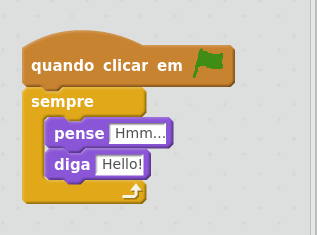
\includegraphics[width=.9\linewidth,fbox]{figs/scratch_blocos.png}
        \caption{Blocos do Scratch}
        \label{scratch_blocks}
    \end{subfigure}%
    \begin{subfigure}{.65\textwidth}
        \centering
        
\includegraphics[width=.9\linewidth,fbox]{figs/scratch_jr.png}
        \caption{Blocos do ScratchJr}
        \label{scratch_jr_blocks}
    \end{subfigure}
    \caption{Blocos do Scratch e do ScratchJr.}
    \sourceauthor
    \label{scratch_scratch_jr_blocks}
\end{figure}

Além dos ambientes gráficos, a programação em blocos também existe em interfaces tangíveis. Os blocos gráficos mitigam a necessidade de digitação, porém ainda dependem do mouse ou telas sensíveis ao toque para arrastar e soltar. Os blocos físicos eliminam essa necessidade, permitindo a manipulação direta e natural. O Osmo (\autoref{osmo_blocks}) é um exemplo de uso de blocos tangíveis de programação. Os blocos são identificados pela câmera de um tablet, e um personagem na tela executa os comandos programados. O Cubetto, já apresentado, utiliza blocos que são encaixados em um painel de madeira (\autoref{cubetto_blocks}).

\begin{figure}[!htbp]
    \centering
    \begin{subfigure}{.56\textwidth}
        \centering
        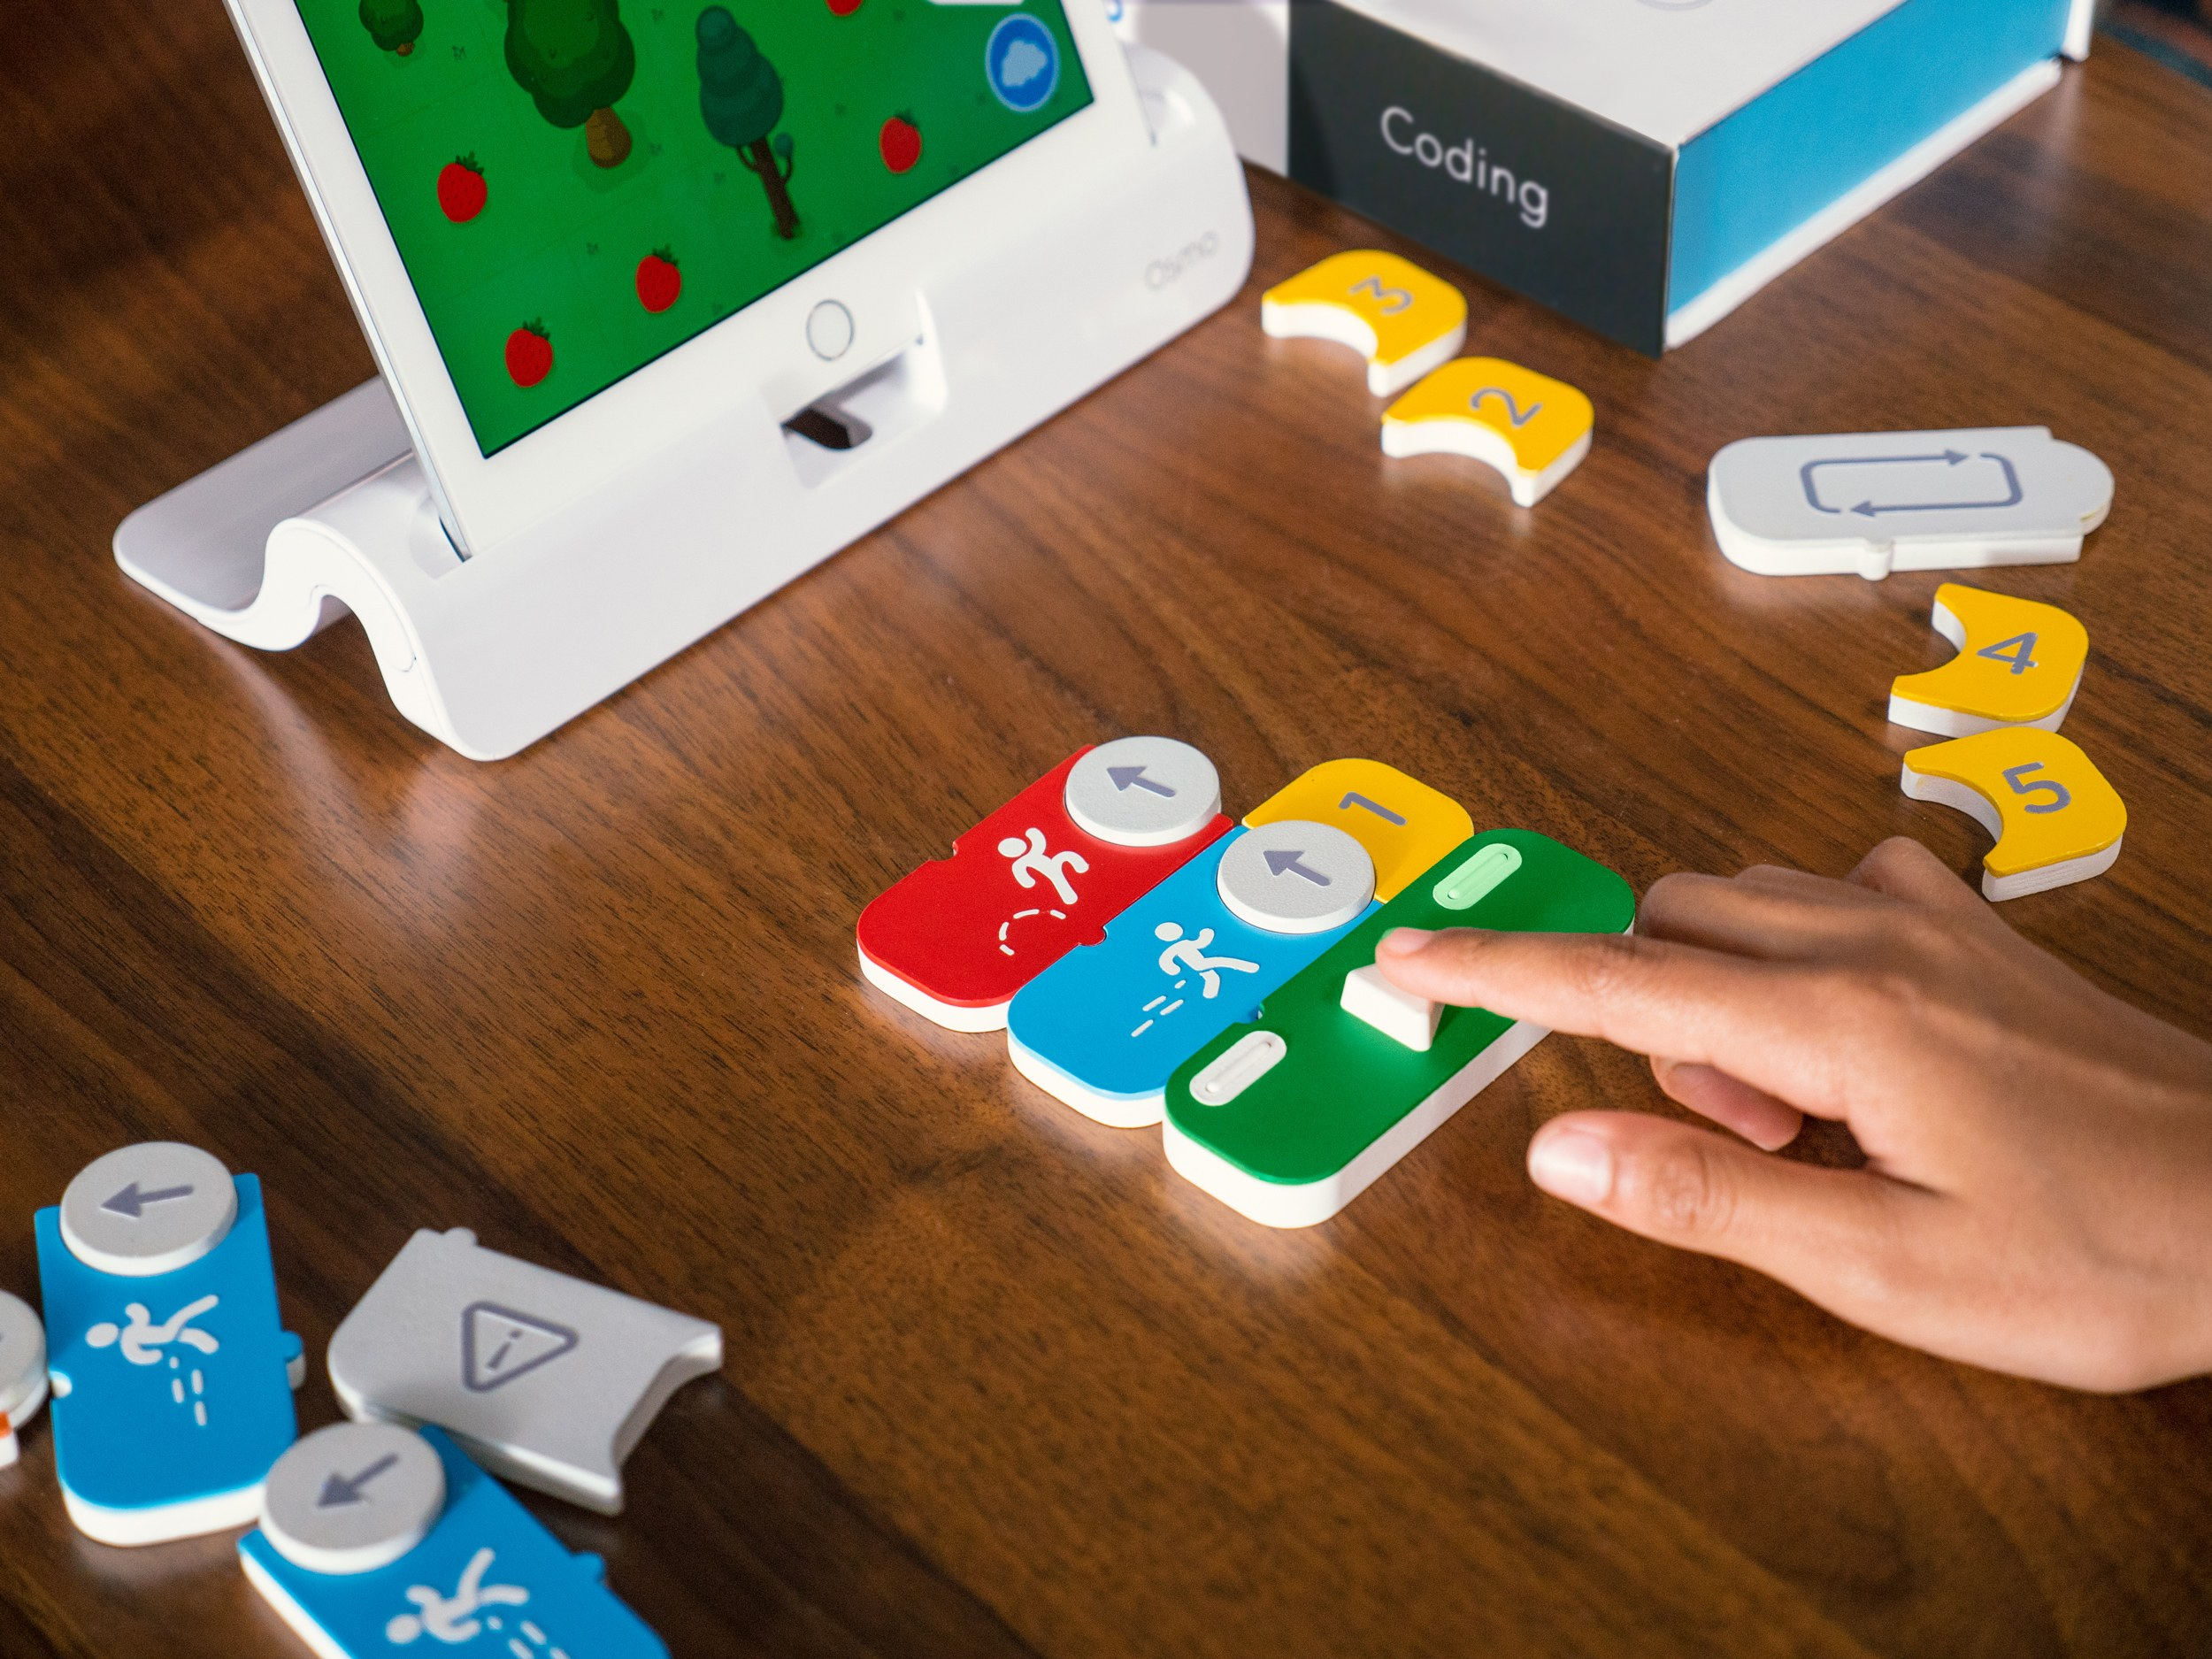
\includegraphics[width=.9\linewidth,fbox]{figs/osmo.jpg}
        \caption{Osmo}
        \label{osmo_blocks}
    \end{subfigure}%
    \begin{subfigure}{.43\textwidth}
        \centering
        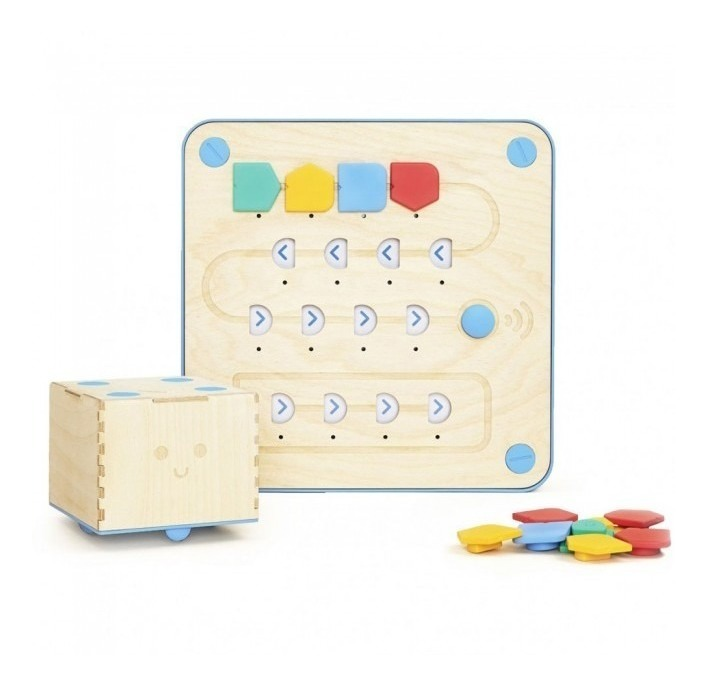
\includegraphics[width=.9\linewidth,fbox]{figs/cubetto.jpg}
        \caption{Cubetto}
        \label{cubetto_blocks}
    \end{subfigure}
    \caption{Blocos tangíveis.}
    \sourceauthor
    \label{tangible_blocks}
\end{figure}

Uma vantagem do painel do Cubetto é indicar, por meio de luzes, qual bloco está sendo executado em cada momento. Isso permite acompanhar a execução, o que é um processo de depuração. Possíveis desvantagens do painel são a limitação do número de encaixes disponíveis e a necessidade de um hardware específico.

\subsection{Marcas Fiduciais}
\label{sub_sec_fiduciais}
Interfaces tangíveis aplicam diferentes técnicas de captura de blocos físicos. O Cubetto depende de um hardware específico para identificar os blocos encaixados em um painel, e o Osmo utiliza visão computacional. Uma alternativa que pode facilitar a demarcação de objetos físicos na construção de interfaces tangíveis, e também na construção de aplicações de Realidade Aumentada (\autoref{sub_sec_fiduciais}), são as marcas fiduciais.

Marcas fiduciais (\autoref{fiducial}) são padrões de figuras desenvolvidas com o objetivo de facilitar a identificação e localização de pontos de referências em imagens. Sistemas de marcas fiduciais são compostos por modelos de marcas e um algoritmo capaz de identificá-las. Apesar de o campo da visão computacional ter evoluído a ponto de não depender de marcas artificiais para detectar objetos, o uso de marcas fiduciais pode aumentar a confiabilidade e velocidade de processamento em sistemas \cite{fiala_designing_2010}.

\begin{figure}[!htbp]
    \centering
    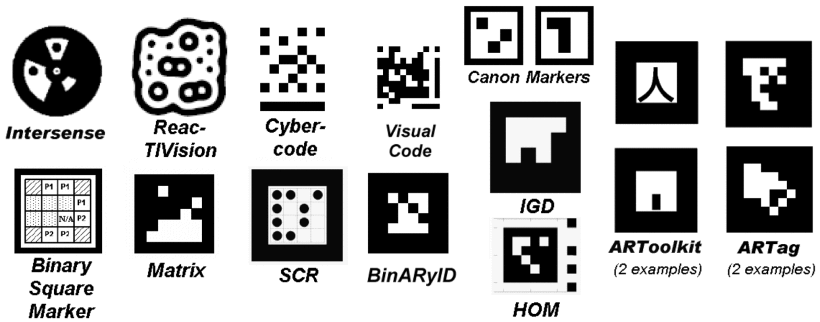
\includegraphics[width=0.9\linewidth,fbox]{figs/fiducial_marks.png}
    \caption{Exemplos de marcas fiduciais.}
    \source{\citeonline{fiala_designing_2010}.}
    \label{fiducial}
\end{figure}

Códigos de barra e QR Codes não são considerados marcas fiduciais. O objetivo destes é carregar informações e não tem dados suficientes para permitir a sua localização. Entretanto, o uso de padrões bitonais (geralmente preto e branco) dos QrCodes e códicos de barra é aproveitado nas marcas fiduciais, dado que isso facilita a detecção quando há variações de luminosidade.

TopCodes\footnote{\url{http://users.eecs.northwestern.edu/~mhorn/topcodes/}} é uma biblioteca de visão computacional projetada para permitir rápida detecção de marcas fiduciais. Além da identificação e da localização, a biblioteca informa o diâmetro e a orientação de cada marca. A biblioteca tem código aberto e é utilizada em diferentes projetos. \citeonline{hu_strawbies_2015} implementaram uma linguagem de blocos tangíveis para programar o personagem do ambiente Osmo (\autoref{strawbies_topcodes}). \citeonline{viana_interface_2018} implementam um ambiente de algoritmos sonoros para deficientes visuais, onde cada marca fiducial representou um instrumento musical (\autoref{bateria_topcodes}).

Uma desvantagem desse tipo de abordagem é o fato de o usuário encobrir as marcas durante a manipulação. A não detecção de uma peça pode prejudicar o desempenho de sistemas que precisam detectar objetos constantemente. Entretanto esse problema não é relatado nos trabalhos mencionados.

\begin{figure}[h!]
    \centering
    \begin{subfigure}{.4\textwidth}
        \centering
        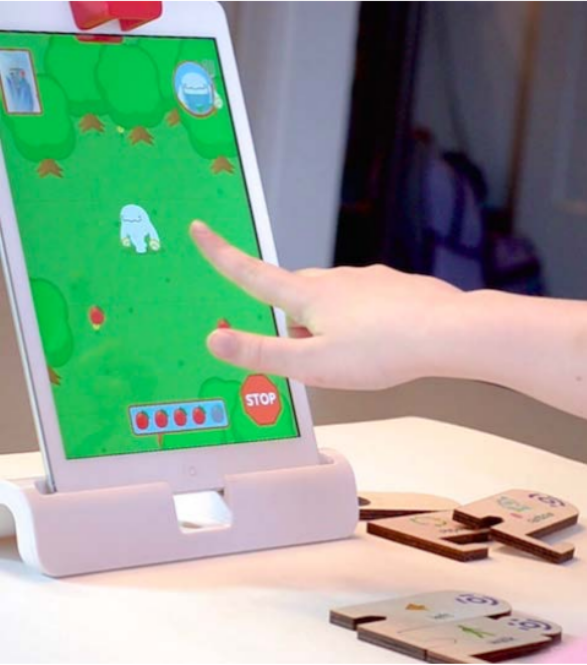
\includegraphics[width=.9\linewidth,fbox]{figs/topcodes_osmo.png}
        \caption{Tablet captura marcas fiduciais}
        \source{\citeonline{hu_strawbies_2015}.}
        \label{strawbies_topcodes}
    \end{subfigure}%
    \begin{subfigure}{.57\textwidth}
        \centering
        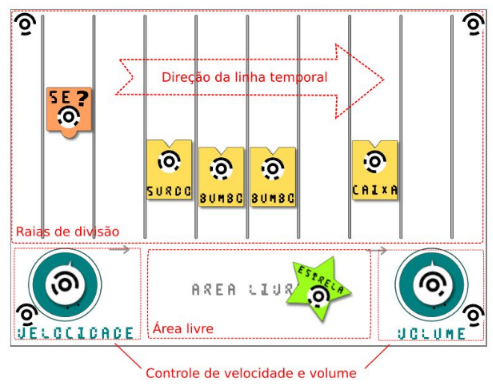
\includegraphics[width=.9\linewidth,fbox]{figs/topcodes_cassiano.png}
        \caption{Bateria de algoritmos sonoros tangível}
        \source{\citeonline{viana_interface_2018}.}
        \label{bateria_topcodes}
    \end{subfigure}
    \caption{Exemplos de uso da biblioteca TopCodes.}
    \label{topcodes_examples}
\end{figure}

\section{Realidade Aumentada}
\label{sec_realidade_aumentada}
A Realidade Aumentada (RA) é uma tecnologia que tem se popularizado nos últimos dez anos. Tem aplicações em inúmeros campos, entre os quais a medicina, a indústria, educação e entretenimento \cite{mekni_augmented_2014}. Apesar da popularização recente, as primeiras experiências com RA são atribuídas a Ivan Sutherland, que na década 1960 criou um dispositivo com pequenas telas próximas aos olhos, que permitiam ver o mundo real e adicionavam objetos virtuais adaptáveis às mudanças de perspectiva do usuário. Ainda hoje a RA se caracteriza por complementar a percepção do usuário ao associar elementos virtuais sobre elementos reais  \cite{parveau_3ivclass_2018}. Além da RA, existem outras técnicas que mostram elementos virtuais e proporcionam experiências realistas de interação, como a Realidade Virtual (RV). Essas técnicas se diferenciam pela quantidade de informação real ou virtual acessada.

Para melhor compreender essa associação \citeonline{milgram_augmented_1994} propõem o conceito de \textit{Virtual Continuum} (\autoref{fig_milgram}). Esse conceito tem de um lado a realidade, e do outro a virtualidade. A realidade está restrita a condições físicas, como gravidade e velocidade. A virtualidade, por outro lado, pode ter suas próprias regras. Entre os dois opostos há um intervalo que mistura real e virtual, denominado Realidade Mista (RM). A RA se encontra à esquerda neste intervalo pois a maior parte da informação acessada pelo usuário existe no ambiente real, e apenas uma camada de objetos virtuais é adicionada. O conceito também apresenta a virtualidade aumentada, que seria a Realidade Virtual. Por ter a maior parte do conteúdo gerado pelo computador e apenas preservar alguns aspectos da realidade, a RV se encontra à direita no intervalo da Realidade Mista.

\begin{figure}[!htpb]
  \centering
  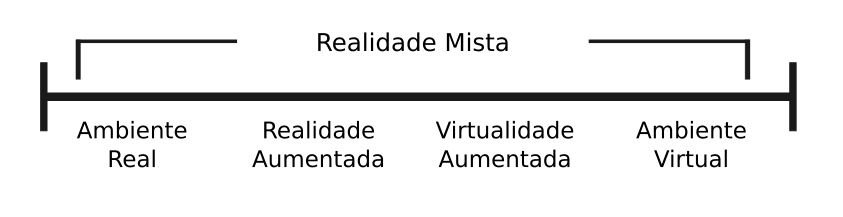
\includegraphics[width=.6\linewidth,fbox]{figs/milgram.png}
  \caption{\textit{Continuum} de realidade-virtualidade de Milgram (1994).}
  \source{Adaptado de \citeonline{milgram_augmented_1994}.}
  \label{fig_milgram}
\end{figure}

%Outra definição Na RV o usuário tem uma experiência realista de interação, porém todos os elementos que ele vê são gerados por computador, sem ter acesso ao mundo real. Essa experiência geralmente é alcançada com dispositivos como óculos e capacetes de visualização \cite{rodello_realidade_2010}. Na RA, ao contrário, o usuário acessa o mundo real e vê objetos virtuais associados a figuras reais que são identificadas por meio de visão computacional. Não há, entretanto, interação direta com os objetos virtuais a não ser movimentando as figuras às quais eles estão atrelados. Já na RM, a diferença é que o usuário pode interagir com os objetos virtuais, o que exige dispositivos especiais de visualização e identificação de gestos \footnote{Um exemplo de dispositivo com realidade mista é o HoloLens \url{https://www.microsoft.com/en-us/hololens}.}.

\citeonline{azuma_recent_2001} acrescenta outros dois princípios além da combinação de objetos virtuais e reais. Primeiro, o sistema deve funcionar de forma iterativa e em tempo real, de modo que as mudanças ocorram instantaneamente. Qualquer modificação de perspectiva ou de posicionamento dos objetos reais deve ser imediatamente refletida nos objetos virtuais percebidos pelo usuário. O segundo princípio define que deve haver um alinhamento dos objetos virtuais com os reais, denominado de \textit{registro}. Ou seja, o posicionamento dos objetos virtuais precisa fazer sentido em relação ao mundo real.

\subsection{Tecnologias para Criar Realidade Aumentada}

Para ser viável, a RA depende de um conjunto de tecnologias para mostrar objetos virtuais e rastrear os objetos reais. A \autoref{subsub_displays} apresenta diferentes tipos de displays e a seção \autoref{subsub_tracking} cita tecnologias de rastreio/registro.

\subsubsection{Displays}
\label{subsub_displays}

Um dos objetivos da RA é produzir integrações de modo que o usuário não consiga distinguir o real do virtual. Diferentes tipos de display tem servido a este propósito. Os displays são responsáveis por dispor o objeto virtual em algum ponto entre a retina do observador e o ambiente real. Eles podem estar ou não acoplados ao observador, ser de uso individual ou permitir interações em grupo. Há três classes principais de dispositivos utilizados para mostrar os objetos virtuais: os \textit{head-worn displays}, os \textit{handheld displays} e \textit{projection displays} \cite{azuma_recent_2001}.

\begin{figure}[h]
    \centering
    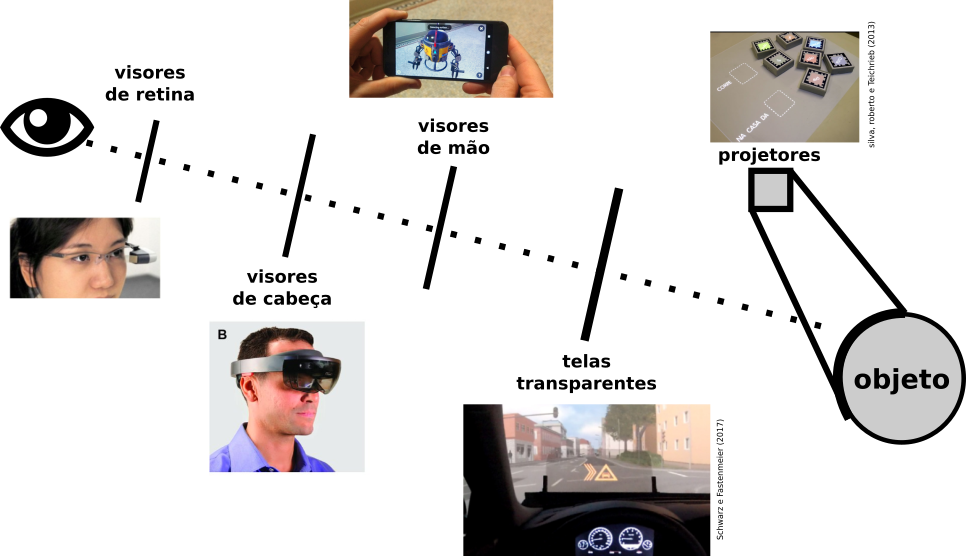
\includegraphics[width=.9\linewidth,fbox]{figs/ra_displays.png}
    \caption{Interseção de objetos virtuais entre o olho humano e o mundo real. }
    \source{Adaptado de Oliver e Raskar (2015).}
    \label{fig:ra_displays}
\end{figure}

\subsubsubsection*{Head-worn displays}

Os \textit{head-worn displays} (visores de cabeça) são usados na cabeça do usuário e mostram imagens em visores próximos aos olhos. Essa abordagem foi utilizada por Ivan Sutherland na primeira aplicação de RA. Esses visores são comumente de dois tipos. O primeiro tipo é um visor transparente, como uma lente de óculos, que permite ver o mundo real e ao mesmo tempo mostra os objetos virtuais. O segundo tipo são visores como telas de LCD. Nessa abordagem uma câmera capta o mundo real e transmite ao usuário por meio do visor, que adiciona os objetos virtuais na cena. \citeonline{azuma_recent_2001} cita um terceiro tipo de display de cabeça que projeta as imagens diretamente na retina humana por meio de \textit{lasers} de baixa potência.

\subsubsubsection*{Handheld displays}

Os \textit{handheld displays} (visores de mão) representam o modo mais comum e acessível de RA. É o que \citeonline{milgram_augmented_1994} denomina \textit{window-on-the-world}, ou seja, uma janela no mundo. Os objetos virtuais aparecem em um visor de um dispositivo que o usuário segura com as mãos (um \textit{smartphone} ou \textit{tablet}), que pode ser comparado a uma lupa. Por meio dessa "janela" ou "lupa" o usuário visualiza o mundo real e os objetos virtuais. Por ser o mais comum, há um conjunto de projetos que visam facilitar o desenvolvimento de aplicações de AR para dispositivos móveis, como o ARCore\footnote{\url{https://developers.google.com/ar}}, da Google.

\subsubsubsection*{Projection Displays}

Os \textit{projection displays} (visores de projeção) projetam a informação virtual diretamente sobre o ambiente físico. No caso mais simples, utiliza-se um ou mais projetores fixos no ambiente. Outra estratégia é utilizar projetores acoplados à cabeça do usuário, mas há a desvantagem do peso do equipamento \cite{azuma_recent_2001}. Ambos os casos precisam considerar as características da superfície de projeção, pois superfícies irregulares tendem a deformar a imagem projetada.

A criação de objetos virtuais que aparecem no mesmo espaço físico que os objetos reais se dá no campo da Realidade Aumentada Espacial. Quando se usa projetores para criar os objetos virtuais, \citeonline{resch_enhancing_2016} denomina como Realidade Aumentada Espacial Projetiva, aqui tratada simplesmente como RA Projetiva. Ele cita como vantagens dessa abordagem:
\begin{itemize}
    \item Não haver erros de profundidade em relação ao ambiente físico, pois os objetos virtuais são projetados diretamente no ambiente;
    \item Ausência de capacetes especiais ou dispositivos que precise segurar com as mãos, aumentando a segurança e liberando ações manuais;
    \item O desacoplamento espacial em relação ao usuário permite que os objetos virtuais sejam acessados por grupos maiores de usuários, o que não ocorre com capacetes ou smartphones;
    \item A resolução obtida com projeção tende a ser maior do que a oferecida por dispositivos acoplados à cabeça.
\end{itemize}

Entretanto há também desvantagens. Ambientes com iluminação forte tendem a ofuscar a imagem projetada, o que exige projetores mais potentes ou projetores a \textit{laser}. O segundo problema é a possibilidade de o usuário obstruir a projeção. Uma forma de mitigar esse problema é o uso de mais de um projetor de maneira sincronizada.

\begin{figure}[h]
    \centering
    \begin{subfigure}{.33\textwidth}
        \centering
        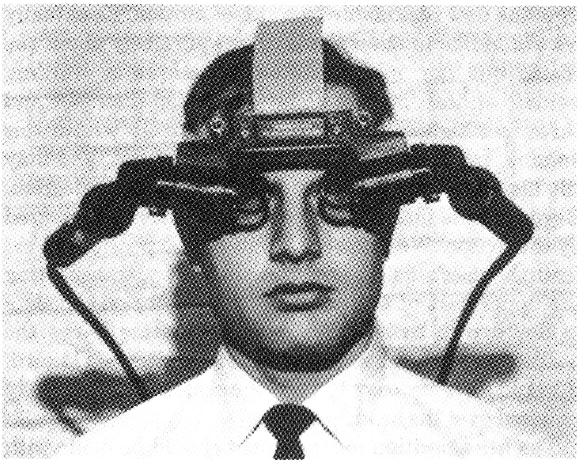
\includegraphics[width=.9\linewidth,fbox]{figs/ivan_sutherland_device.png}
        \caption{Visor de cabeça criado por Ivan Sutherland em 1968.}
        \label{fig_ivan_sutherland}
        \source{\citeonline{sutherland_head-mounted_1968}.}
    \end{subfigure}%
    \begin{subfigure}{.55\textwidth}
        \centering
        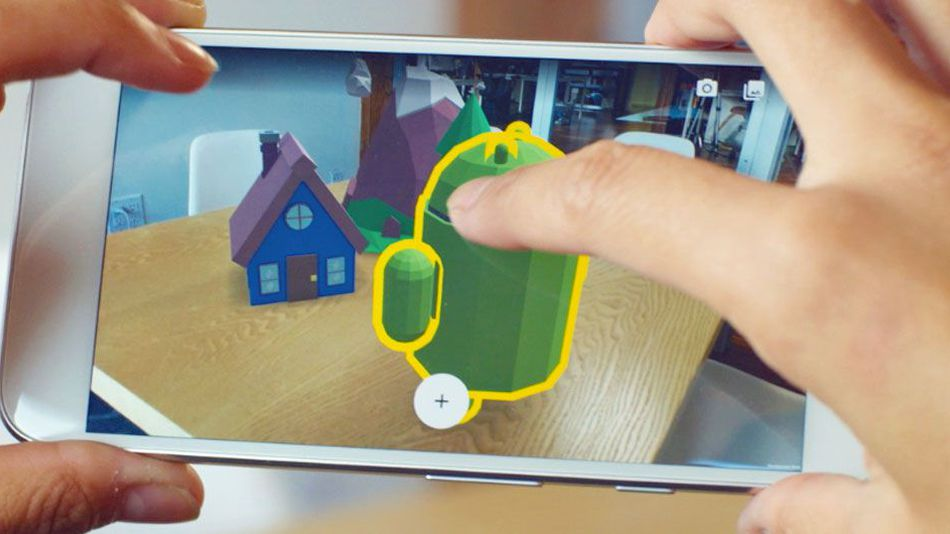
\includegraphics[width=.9\linewidth,fbox]{figs/arcore.jpg}
        \caption{Visor de mão, em aplicação para smartphone criada com ARCore.}
        \label{fig_arcore}
    \end{subfigure}%
    \caption{Dispositivos para criar realidade aumentada.}
    \label{fig_ra_devices}
\end{figure}

\subsubsection{Tecnologias de Rastreamento}
\label{subsub_tracking}
O rastreio do usuário, dos objetos virtuais e dos objetos reais, é um aspecto crucial para criar aplicações de RA convincentes \cite{bimber_spatial_2005}. Um conjunto de métodos são utilizados para esse rastreamento, com base em sensores como giroscópios, acelerômetros e sensores magnéticos, mas a maior parte se baseia em captação de imagem \cite{resch_enhancing_2016}. As seguir são apresentadas brevemente duas técnicas de rastreamento com captação de imagem.

\subsubsubsection*{Marcas Fiduciais}

As abordagens de rastreamento com base em captação de imagem precisam extrair características presentes na cena observada. Essas características podem ser naturais ou implantadas artificialmente em pontos de interesse. As marcas fiduciais são exemplos de características artificiais que são reconhecidas com mais facilidade por algoritmos de visão computacional. Essas marcas, apresentadas na \autoref{sub_sec_fiduciais}, além de serem utilizadas em aplicações com interfaces tangíveis, são amplamente aplicadas na RA.

O processo de identificação das marcas artificiais inicia com a captura da imagem, à qual aplica-se um filtro para transformá-la em preto e branco. Segundo \citeonline{resch_enhancing_2016} essa etapa é complexa devido à variações de luminosidade do ambiente. Depois deste filtro, são extraídos os contornos das marcas e por fim o código binário de cores interno à cada marca é decodificado.
No campo da RA projetiva, uma desvantagem do uso de marcas especiais é o fato da projeção alterar as características da marca, principalmente as cores, prejudicando sua identificação. Para evitar esse problema é necessário desativar a projeção enquanto a câmera capta as marcas, mas isso impede a projeção em tempo real \cite{resch_enhancing_2016}.

\subsubsubsection*{Características Naturais}
As características naturais são estruturas que pertencem à cena sem em si, ou seja, não há modificações artificiais para facilitar sua identificação. Essas características precisam, assim como as marcas fiduciais, ser identificáveis em condições de iluminação e posições diversas. Há dois tipos de rastreio naturais, os quais buscam identificar bordas e pontos.

A identificação de bordas foi um dos primeiros métodos de rastreio de características naturais utilizados, pela facilidade de identificação e robustez em condições variantes de iluminação. Nessa técnica, uma câmera capta um quadro da cena, que é comparado com um modelo 3D do objeto a ser identificado. Essa comparação tem como saída a estimativa da posição atual do objeto \cite{resch_enhancing_2016}.

Por outro lado, a identificação de pontos é uma alternativa que também é robusta a variações de luminosidade. Pontos de interesse são previamente cadastrados em uma base de dados criada a partir de um modelo 3D observado de diferentes pontos de vista. Os mesmos pontos são, posteriormente, extraídos da imagem captada pela câmera, e comparados aos pontos armazenados. Essa busca permite então encontrar a posição atual aproximada do objeto real.

\subsection{RA Projetiva}
\label{sub_aplicacoes_ra_projetiva}

A RA projetiva é um subtipo da Realidade Aumentada Espacial, a qual normalmente associa um ou mais projetores para produzir o conteúdo virtual e câmeras para captar os objetos reais. \citeonline{bimber_spatial_2005} comentam que os ambientes com uso de projeção se popularizaram na década de 1990. Um exemplo desta época é o CAVE, um quarto cujas paredes serviam de telas para criar uma experiência imersiva. Outros exemplos, com menos imersão, tem projeção em áreas menores, como mesas, paredes, paredes curvadas e esferas.

A RA projetiva tem encontrado aplicações em áreas diversas. Uma das abordagens é simular a visualização de estruturas internas à uma superfície, para facilitar o manuseio das mesmas sem a necessidade de abrir a superfície. Exemplos são órgãos humanos, no campo da medicina, e peças de veículos, na mecânica. Em um trabalho neste sentido, \citeonline{bornemann_exploration_2020} combinam três projetores apontados para um manequim e projetam os órgãos humanos permitindo estudar sua localização (\autoref{fig_bornemann}). Essa projeção se modifica conforme os movimentos da cabeça do observador, dando às estruturas projetadas um aspecto tridimensional. Essa técnica potencialmente facilitaria cirurgias não invasivas, nas quais atualmente o cirurgião divide a atenção entre o corpo do paciente e um monitor. A projeção dos órgãos sobre o corpo do paciente evitaria a divisão de atenção, mantendo os olhos direcionados para um único local.

Outra aplicação na área médica é o tratamento de pacientes com fobias de pequenos animais. \citeonline{wrzesien_treating_2015} usam um projetor para mostrar os animais que o paciente teme e ele pode interagir com os mesmos de forma controlada (\autoref{fig_wrzesien}). No campo da indústria, \citeonline{sand_smartassembly_2016} desenvolveram o smARt.assembly, que é um sistema de assistência à trabalhadores responsáveis por montagens manuais. O sistema tem um projetor apontado para uma estante com peças, onde destaca a próxima peça a ser utilizada e também mostra como encaixá-la no produto a ser montado (\autoref{fig_sand}).

\begin{figure}
    \centering
    \begin{subfigure}{.33\textwidth}
        \centering
        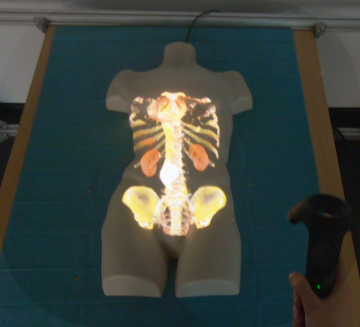
\includegraphics[width=.9\linewidth,fbox]{figs/bornemann.png}
        \caption{Projeção de órgãos internos.}
        \label{fig_bornemann}
        \source{\citeonline{bornemann_exploration_2020}.}
    \end{subfigure}%
    \begin{subfigure}{.33\textwidth}
        \centering
        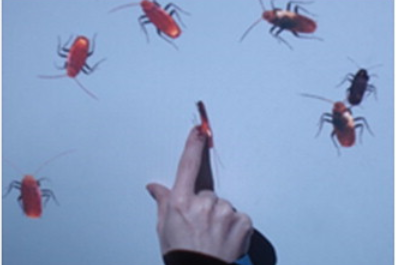
\includegraphics[width=.9\linewidth,fbox]{figs/wrzesien.png}
        \caption{Tratamento de fobias.}
        \label{fig_wrzesien}
        \source{\citeonline{wrzesien_treating_2015}.}
    \end{subfigure}%
    \begin{subfigure}{.33\textwidth}
        \centering
        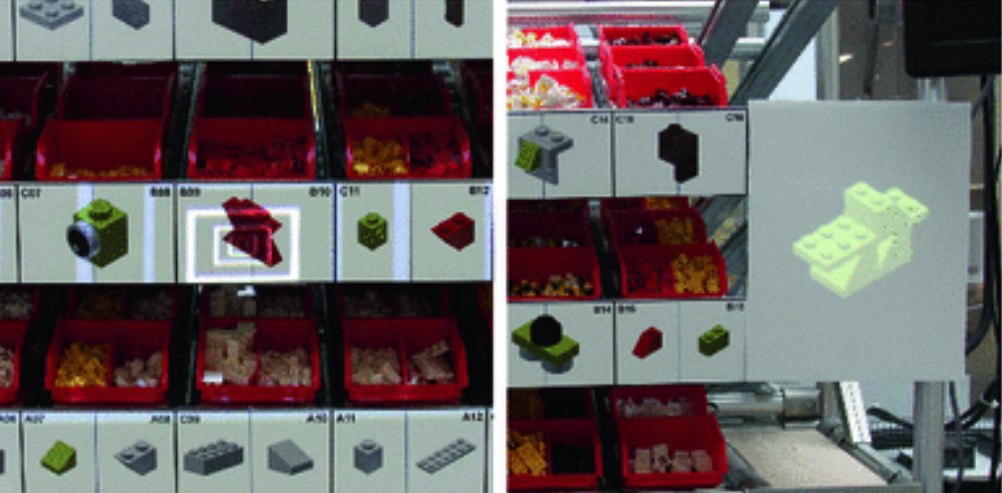
\includegraphics[width=.9\linewidth,fbox]{figs/sand.png}
        \caption{Auxílio em linhas de montagem.}
        \label{fig_sand}
        \source{\citeonline{sand_smartassembly_2016}.}
    \end{subfigure}%
    \caption{Aplicações de RA Projetiva.}
    \label{fig_proj_ra_applications}
\end{figure}

\subsubsection{RA Projetiva Aplicada a Ferramentas Educacionais}
\label{sub_sub_aplicacoes_ra_projetiva_educacao}

A \ac{RA} tem potencial educacional ao motivar os estudantes e promover a interação entre o conteúdo e o aluno \cite{silva_evaluating_2013}. Portanto, além das aplicações na medicina e na indústria, a RA projetiva também se aplica a ferramentas educacionais. Além da RA projetiva, essas ferramentas normalmente utilizam elementos tangíveis que servem como entradas para sistemas câmera-projetor. Câmeras captam os elementos tangíveis e algoritmos de visão computacional identificam esses elementos analisando suas marcas especiais ou suas características naturais. Como saída, um projetor emite os elementos virtuais.

A vantagem de unir a RA projetiva com interfaces tangíveis em aplicações educacionais está no favorecimento das interações em grupo. Sabe-se que as interações sociais favorecem o aprendizado por meio do \textit{scaffolding} (\autoref{sub_jerome_bruner}). A combinação \textit{RA projetiva-interfaces tangíveis} favorece interação em grupo de dois modos. Por um lado, a RA projetiva mostra os objetos virtuais a mais de um usuário ao mesmo tempo. Por outro lado, as interfaces tangíveis permitem a manipulação de objetos físicos por mais de um usuário simultaneamente \cite{burleson_active_2018, horn_tangible_2012}.

\begin{figure}[h]
    \centering
    \begin{subfigure}{.49\textwidth}
        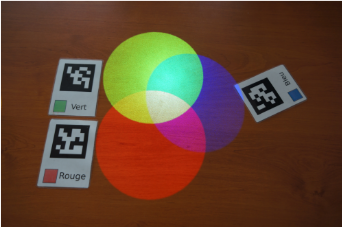
\includegraphics[width=.9\linewidth,fbox]{figs/nectar.png}
        \caption{Nectar - Exploração de modos de cores.}
        \label{fig_nectar}
        \source{\citeonline{laviole_nectar_2018}.}
    \end{subfigure}
    \begin{subfigure}{.49\textwidth}
        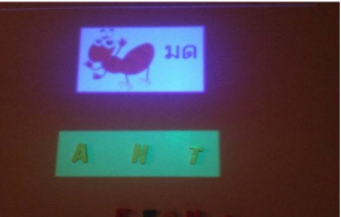
\includegraphics[width=.9\linewidth,fbox]{figs/pinkaew.png}
        \caption{Tangible Word Game - Alfabetização.}
        \source{\citeonline{pinkaew_interactive_2014}.}
        \label{fig_pinkaew}
    \end{subfigure}
    \begin{subfigure}{.49\textwidth}
        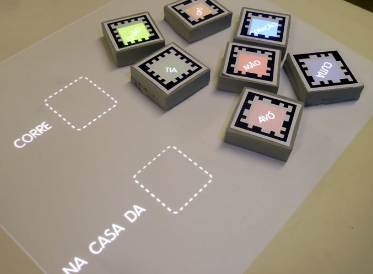
\includegraphics[width=.9\linewidth,fbox]{figs/roberto.png}
        \caption{ARBlocks - Atividade de alfabetização.}
        \label{fig_silva_roberto_ra}
        \source{\citeonline{silva_evaluating_2013}.}
    \end{subfigure}
    \begin{subfigure}{.49\textwidth}
        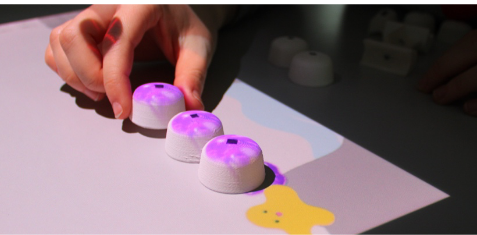
\includegraphics[width=.9\linewidth,fbox]{figs/mart.png}
        \caption{MaR-T - Atividade de matemática.}
        \label{fig_math}
        \source{\citeonline{besevli_mar_t_2019}.}
    \end{subfigure}
    \caption{Ferramentas educacionais usando RA projetiva.}
\end{figure}

\citeonline{laviole_nectar_2018} apresenta uma ferramenta para exploração de modelos de cores aditivas e subtrativas (\autoref{fig_nectar}). A soma das cores primárias no modo aditivo (verde, vermelho e azul) resulta em branco, e a soma das cores primárias no modo subtrativo (ciano, magenta e amarelo) resulta em preto. Na ferramenta de Laviole, cartas com marcas fiduciais representam as cores, e ao lado de cada carta é projetado um círculo colorido que pode ser sobreposto a outros círculos. Além disso, há uma carta que permite trocar entre o modo aditivo e o subtrativo. Um questionário guia os estudantes na exploração das cartas, com perguntas como: o que é a cor branca? o que você vê ao combinar vermelho, verde e azul? Tentando responder as perguntas, os estudantes exploram as combinações de modo ativo e colaborativo, possivelmente compreendendo esse fenômeno físico complexo.

Outras duas ferramentas visam promover a alfabetização. \citeonline{pinkaew_interactive_2014} identificam sequências de letras de plástico e projetam figuras referentes às palavras formadas. Uma câmera de infravermelho capta as letras, técnica que apresentou problemas de diferenciação de letras similares como Q, O, e C, devido à fontes de luz inadequadas. A segunda ferramenta é o ARBlocks, desenvolvido por \citeonline{roberto_dynamic_2013}. O ARBlocks possui blocos tangíveis customizáveis via projeção de conteúdo virtual, bem como feedbacks luminosos e sonoros. A atividade proposta consistiu na formação de rimas ao completar frases com blocos tangíveis (\autoref{fig_silva_roberto_ra}). A avaliação com grupo de teste e de controle concluiu que o grupo de teste, que tinha dificuldade de aprendizado, conseguiu obter aprendizados semelhantes ao grupo de controle nos assuntos que foram abordados usando RA. A professora da turma também mencionou motivação e engajamento das crianças no uso da ferramenta, a qual afirma tê-las incentivado a lerem mais.

A última ferramenta de exemplo aborda o conteúdo de matemática com o objetivo de auxiliar crianças de 3 a 5 anos no desenvolvimento da representação numérica não-simbólica, ou seja, a comparação entre grandezas (tamanhos, quantidades) antes do reconhecimento dos símbolos numéricos. Denominada MaR-T, a ferramenta desenvolvida por \citeonline{besevli_mar_t_2019} mostra uma sequência de atividades nas quais a criança agrupa pedrinhas de modo a permitir a passagem de um personagem virtual sobre buracos e rios. As pedras são empilhadas, na horizontal ou agrupadas para a criança compreender a conservação de quantidades em diferentes disposições. Em cada etapa, a criança coloca a mão sobre o grupo que possui mais ou menos peças. Em termos de hardware e software, a aplicação utiliza um projetor acoplado a um \textit{smartphone} Android, e as peças utilizam adesivos refletores que facilitam a identificação por meio da biblioteca OpenCV.

\subsubsection{Métodos de Entrada}
Os métodos de entrada desses sistemas são diversos. No caso do smaArt.assembly o trabalhador controla o sistema por meio de pedais, para não perder tempo de trabalho manual. Já o sistema de \citeonline{bornemann_exploration_2020} combina a captação de movimentos da cabeça do usuário por meio de controles remotos que tem sua posição rastreada por sistemas específicos. Ambos os trabalhos citam o reconhecimento de gestos como um método de entrada alternativo a ser testado futuramente. Já o trabalho de \citeonline{wrzesien_treating_2015} reconhece gestos captados por uma câmera, de modo que o paciente pode interagir com os animais projetados colocando a mão sobre eles. Métodos de entrada tradicionais também são aplicados. Plecher et al (2020) usam RA projetiva em uma exposição de museu, na qual os usuários interagem por meio de um \textit{tablet} para pintar uma estátua em exposição, de modo que as cores selecionadas no aparelho se refletem na escultura por meio de um projetor. Por fim, as ferramentas educacionais apresentadas (\autoref{sub_sub_aplicacoes_ra_projetiva_educacao}) tem em comum o uso de interfaces tangíveis com ou sem marcas fiduciais, que são identificadas por meio de câmeras.

\section{Considerações}

Este capítulo abordou temas fundamentais para guiar a criação de interfaces de programação para crianças. Olhar para o indivíduo que usará uma ferramenta, pensando no seu desenvolvimento cognitivo, limitações motoras e aspectos emocionais é a direção apontada por Montessori, Piaget, Bruner e Papert.

A segunda seção (\autoref{fundamentacao_pc}) abordou a definição de \acl{PC}. Apesar da falta de uma definição estabelecida, percebe-se que há grande relação com programação, mas que também vai além dela. Os pilares de decomposição, reconhecimento de padrões e abstração podem ser aplicados em resolução de problemas por vezes sem o uso de dispositivos computacionais. A depuração, por estar associada à tarefa de programar, por vezes tem importância secundária e não é mencionada em definições do PC.

A seguir foram abordadas duas classificações de brinquedos programáveis e diferentes alternativas tecnológicas empregadas em suas interfaces. Percebe-se que os autores incentivam o uso de interfaces tangíveis para crianças, e que a programação em blocos é a metáfora mais utilizada para representar comandos. Percebe-se a preocupação com o design dos blocos, que ao evitar o uso de letras considera se o público é ou não alfabetizado.

Um último item abordado foram novas formas de interação: interfaces de realidade virtual, aumentada e mista. Como demonstrado no próximo capítulo, poucos brinquedos programáveis utilizam esse tipo de interface, e portanto investigar a adequação dessas tecnologias para o público infantil é um tema a ser explorado.
\chapter{Trabalhos Relacionados}
\label{c_estado_arte}

Este capítulo apresenta trabalhos similaridades ao que se propõe nesta pesquisa. Ele está dividido em três seções. A \autoref{sec_tools} apresenta ferramentas que buscam auxiliar crianças nos primeiros contatos com algoritmos por meio da depuração. A \autoref{sec_rsl} apresenta uma revisão sistemática da literatura (RSL) sobre pesquisas que observam a interação de crianças de 3 a 6 anos com BPs. A intenção é compreender quais interfaces são comumente utilizadas, quais são os designs experimentais aplicados e que resultados são obtidos, para fundamentar a escolha do design experimental desta pesquisa. Por fim, a \autoref{secao_mapeamento_industrial} apresenta um mapeamento industrial\footnote{Método de busca baseado em fontes não acadêmicas, mas que segue um método sistemático. Também chamado de mapeamento industrial sistemático.} sobre as interfaces de BPs que demonstra quais tipos de interface estão disponíveis no comércio eletrônico. %Enquanto na \autoref{sub_sub_aplicacoes_ra_projetiva_educacao} apresenta aplicação de RA projetiva em ferramentas educacionais, o mapeamento indica que a técnica   no contexto de BPs.

\section{Interfaces de Brinquedos Programáveis}
\label{sec_tools}
Esta seção tem por objetivo demonstrar interfaces para crianças terem os primeiros contatos com algoritmos utilizando BPs, e também abordem o tema da depuração. Para isso, identifica as características de cada trabalho e compara com a solução proposta. Os critérios utilizados para a escolha dos trabalhos relacionados foram o público-alvo (crianças a partir dos 4 anos), a visibilidade dos algoritmos por meio de interfaces tangíveis e o uso de BPs. Assim, foram analisados quatro trabalhos:

\begin{enumerate}
    \item Robo-Blocks: uma interface tangível eletrônica para programação de BPs, com foco em ensino de depuração \cite{sipitakiat_robo-blocks_2012}.
    \item Cubetto: um BP com interface tangível de painel, que indica a execução de cada comando por meio de luzes (\url{https://www.primotoys.com}).
    \item Bee-Bot com mesa interativa: uma mesa interativa com objetos tangíveis, que projeta um mapa interativo que reage aos posicionamento dos objetos físicos em sua superfície \cite{beraza_soft_2010}. 
    \item ALERT: interface de programação interativa, na qual o BP interpreta comandos a medida que os detecta via câmera \cite{burleson_active_2018}. 
\end{enumerate}

\subsection{Robo-Blocks}
O Robo-Blocks, de \citeonline{sipitakiat_robo-blocks_2012}, é um sistema que permite que crianças comandem um BP por meio do encaixe de blocos eletrônicos. Os quatro movimentos básicos do robô são iguais aos do brinquedo RoPE (mover-se para frente, para trás, girar à esquerda e girar à direita), porém as crianças também podem parametrizar a extensão do movimento do robô ajustando um controle giratório presente em cada bloco (\autoref{fig:robo_blocks}). Os blocos são encaixados por conectores magnéticos, formando uma sequência. Essa sequência se liga a um bloco principal, que envia os comandos ao BP por comunicação sem fio. O BP, por sua vez, é inspirado na tartaruga do ambiente Logo. Ele tem uma caneta acoplada que permite desenhar ao serem utilizados blocos de \textit{"pen up"} (erguer caneta) e \textit{"pen down"} (baixar caneta).

\begin{figure}[!h]
    \centering
    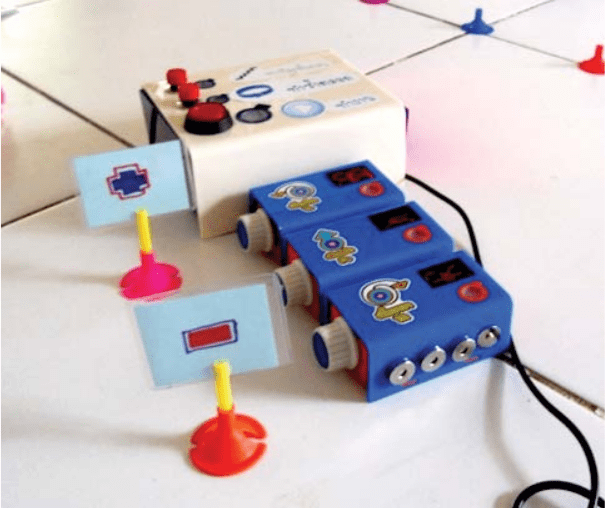
\includegraphics[width=.7\linewidth,fbox]{figs/robo_blocks.png}
    \caption{Robo-Blocks.}
    \label{fig:robo_blocks}
\end{figure}
O Robo-Blocks foi inicialmente desenvolvido com uma interface tangível sem atenção ao processo de depuração. Entretanto os pesquisadores perceberam que as crianças costumavam direcionar sua atenção para os movimentos do robô, sem prestar atenção nos blocos, o que dificultava encontrar erros. Para resolver este problema os autores criaram a função de execução passo a passo, que permite gerenciar a execução e encontrar erros com mais facilidade.

Além da execução passo a passo, os autores utilizam "objetos passivos", ou seja, que não influenciam na execução do robô. No caso foi utilizado pequenas bandeiras com as quais a criança identifica os blocos que podem ser a causa de erros. As bandeiras tem ícones de "mais"\ e "menos". Deste modo, a criança pode colocar a bandeira com sinal positivo ao lado do bloco para indicar que o robô deve girar mais ou mover-se mais para frente, por exemplo. 

Outro objeto utilizado para auxiliar na depuração foi o protractor. Destinado à solucionar dúvidas com relação à ângulos, é um simples pedaço de papel com um furo no centro, por onde o robô passa. Quando o robô está parado, a criança coloca o protractor na mesa, sobre o robô. Ao redor do furo há marcações de ângulos, de modo que a criança consegue estimar o quanto o robô precisa se mover relativo à sua direção atual.

Testes com o Robo-Blocks ocorreram com crianças de 5 a 12 anos, porém o estudo formal focou em crianças de 8 a 9. Esse estudo consistiu em atividades de programar o robô para desenhar a primeira letra do nome e andar em um mapa. Os autores identificaram que as crianças tiveram dificuldades em concluir as atividades e recorreram às funções de depuração. Um problema estava no fato de a criança não conseguir observar a cadeia de comandos e robô simultaneamente. Neste sentido, a execução passo a passo foi o modo de preferido pelas crianças. O uso das bandeiras para marcar os erros também foi comum, porém os autores ressaltam que a presença de um erro no início da cadeia de blocos interfere em todos os demais movimentos do robô, de modo que parecem também estar errados. Essa característica levava as crianças a marcar todos os demais blocos como errados. Neste caso os pesquisadores precisaram intervir corrigindo a posição do robô manualmente.

\subsection{Cubetto}
\label{sub_sec:cubetto}
O Cubetto é um brinquedo programável feito de madeira e destinado a crianças entre 4 a 8 anos, que foi desenvolvido pela empresa PrimoToys\footnote{\url{https://www.primotoys.com}} a partir de 2013. Ele se inspira no ambiente LOGO, pois se move no chão como a tartaruga robótica desenvolvida de Papert. Além disso, o seu design é inspirado no método Montessori, que incentiva o aprendizado autônomo por meio da interação com materiais concretos, lúdicos.

Os algoritmos que definem os movimentos do Cubetto são feitos com blocos coloridos encaixados em um painel. Há 7 tipos de blocos, sendo quatro blocos direcionais e três blocos lógicos. Os blocos direcionais são frente (verde), trás (roxo), giro à esquerda (amarelo) e giro à direita (vermelho). Os blocos lógicos são movimento aleatório (preto), negação (marrom) e função (azul). O bloco de movimento aleatório sorteia um movimento direcional, possibilitando trajetos diferente com um mesmo algoritmo. O bloco de negação é associado a um bloco de movimento, modificando-o para movimento contrário. Por exemplo, se o próximo bloco é girar para a esquerda, então o brinquedo gira para a direita. Por fim, o bloco de função faz com que os blocos encaixados em uma área inferior do painel (área de função) sejam executados. Esses blocos especiais, portanto, permitem estender o comportamento além de sequencias de comandos. Um bloco de função posicionado na área de função, por exemplo, cria uma função recursiva. Se esta função tiver um bloco de movimento aleatório, o brinquedo executará movimentos diferentes indefinidamente.

\begin{figure}
    \centering
    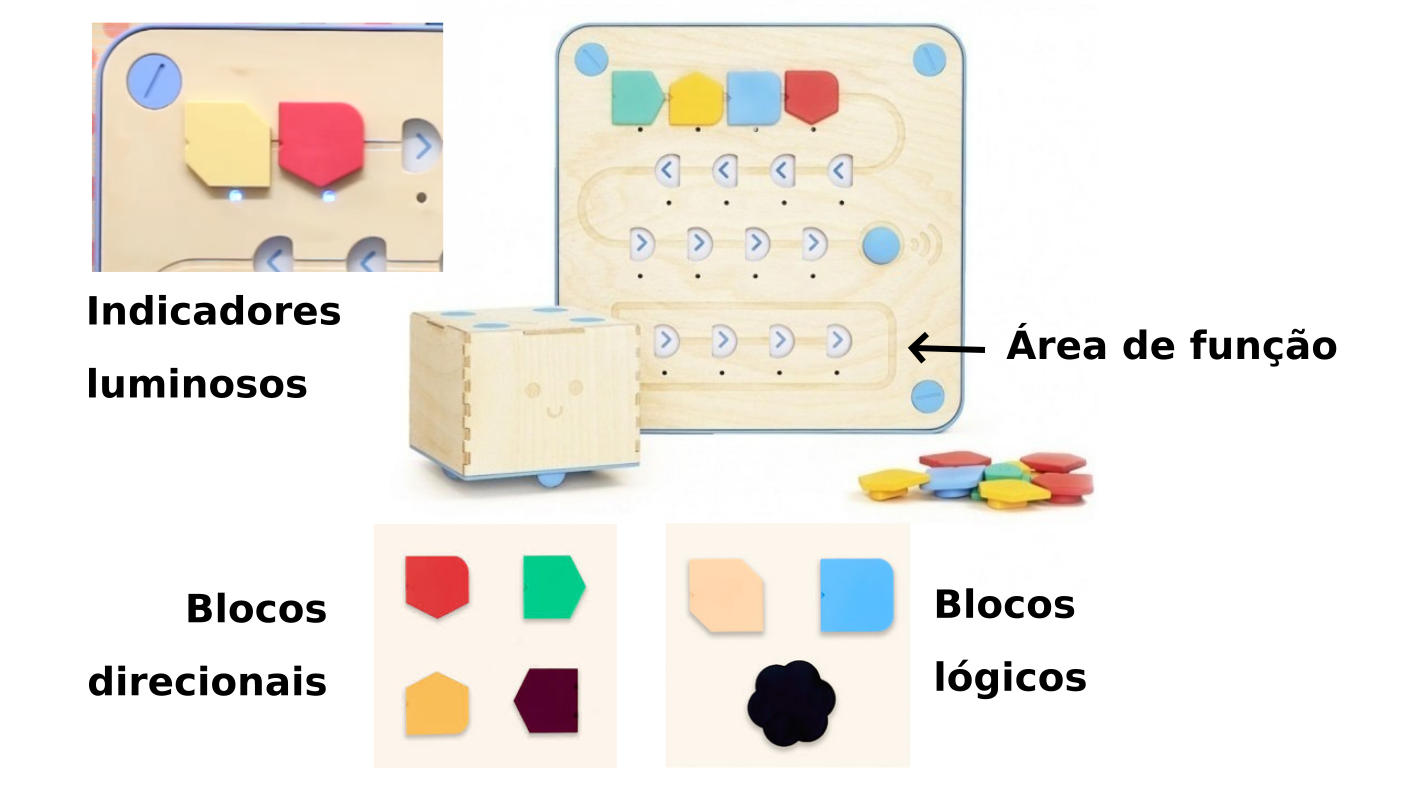
\includegraphics[width=.7\linewidth,fbox]{figs/cubetto_blocks.png}
    \caption{Cubetto: indicadores luminosos, área de função e blocos.}
    \label{fig:cubetto_features}
\end{figure}

O painel do Cubetto possui 16 reentrâncias para encaixe dos blocos, sendo 12 reservadas para o algoritmo principal e 4 dedicadas à área de função. Para cada reentrância há um indicador luminoso que acende quando o bloco é encaixado e pisca quando o bloco é executado. Essa indicação luminosa mostra a sequência de execução de cada bloco, o que é particularmente útil para os blocos de negação e de função. Como o bloco de negação tem sua ação associada ao bloco seguinte (inverte a ação do bloco seguinte), ambos piscam. O mesmo ocorre com o bloco de função, que pisca enquanto os blocos na área de função são executados.

Neste sentido, o design do Cubetto busca tornar visível tanto as instruções do algoritmo quanto destacar cada passo durante a execução. A estrutura é visível por meio dos blocos e do \textit{feedback} luminoso fornecido ao encaixar um bloco no painel. Já a execução é indicada por meio do piscar embaixo de cada bloco. Essa visibilidade facilita a interação das crianças e a formação do modelo mental sobre como as peças se relacionam e modificam o comportamento do brinquedo. Os movimentos lentos do brinquedo, associados a indicação de quais peças estão sendo executadas beneficiam o entendimento do algoritmo e facilitam a depuração. Essas característica fizeram o projeto receber diversos prêmios de design\footnote{
\begin{itemize}
    \item London Design Award (2016) - \url{https://drivenxdesign.com/LON16/project.asp?ID=15112}
    \item German Design Award (2017) - \url{https://www.german-design-award.com/en/the-winners/gallery/detail/9304-cubetto.html}
    \item RedDot Award (2016) - \url{https://www.red-dot.org/project/cubetto-26086}
\end{itemize}
}.

\subsection{Bee-Bot com mesa interativa}
\citeonline{beraza_soft_2010} criaram uma mesa interativa para ser utilizada com a Bee-Bot por crianças de 4-5 a 12-14 anos. Essa mesa tem superfície semitransparente, na qual um projetor cria mapas virtuais interativos, projetando-os por baixo. A imagem projetada muda de acordo com os movimentos da Bee-Bot e acompanha a manipulação de outros elementos tangíveis. Por exemplo, quando a Bee-Bot passa de um quadrado para outro do mapa projetado, este quadrado é destacado.

A projeção de elementos virtuais de acordo com os elementos tangíveis ocorre devido à marcas fiduciais da biblioteca reacTIVision coladas na parte inferior desses elementos. Como a superfície da mesa é semitransparente, uma câmera embaixo da mesa consegue captar as marcas fiduciais. As imagens captadas são analisadas por um software que controla as projeções.

Além da mesa, o trabalho propõe a criação de um software de apoio aos professores para que criem e configurem as atividades com o brinquedo programável. Esse software busca atender aos seguintes requisitos:

\begin{itemize}
    \item Ter tapetes ou cenários adaptados para cada atividade;
    \item Poder interromper uma atividade e continuar depois;
    \item Registrar o progresso das crianças em determinado problema e acompanhar sua evolução no tempo;
\end{itemize}

\begin{figure}[!h]
    \centering
    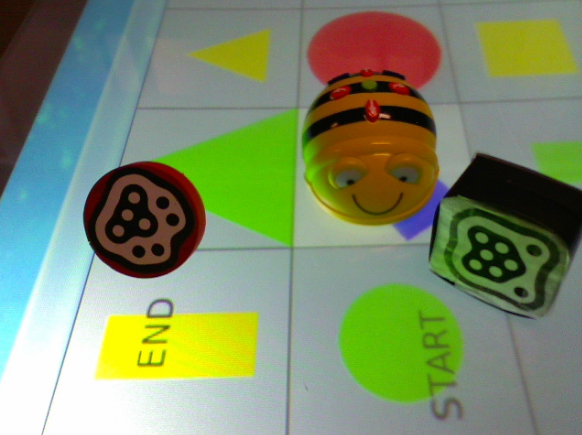
\includegraphics[width=.6\linewidth,fbox]{figs/beraza_bee_bot.png}
    \caption{Mesa interativa com a Bee-Bot.}
    \label{fig:beraza}
    \source{\citeonline{beraza_soft_2010}}
\end{figure}

Uma atividade de demonstração permite entender as potencialidades da tecnologia (\autoref{fig:beraza}). Nessa atividade, o usuário pode decidir o mapa a ser utilizado; decidir as posições de início e fim do trajeto a ser percorrido; e ver o trajeto percorrido com o número de passos executados. A visualização do trajeto percorrido permite à criança refletir sobre os comandos inseridos e depurar possíveis erros.

Nessa demonstração cada quadrado do mapa contém uma forma geométrica de cor e tamanho variado. Isso possibilita que a criança exercite a classificação e abstração. A classificação seria a habilidade de identificar propriedades ou categorias, e relacionar essas categorias ou classes entre si. Nessa atividade, a criança classifica formas geométricas por propriedades como cor, formato e tamanho. Assim, a criança aprende abstrair e observar apenas as propriedades relevantes para formar uma categoria. Esse mesmo tipo de tapete com formas geométricas é utilizado pelo brinquedo RoPE, porém em seu formato físico.

\subsection{ALERT}

O ALERT \cite{burleson_active_2018}, assim como os trabalhos anteriores, é uma interface de programação de brinquedos programáveis. O seu diferencial é que o robô interpreta os comandos a medida que ficam acessíveis no seu campo de visão. Cada robô possui uma câmera, que detecta novos comandos quando o robô se move. Por exemplo, se o robô anda para frente e capta o comando “vire 90º à direita”, ele interpreta e executa esta ação. Nisto percebe-se o princípio do feedback imediato defendido por \citeonline{norman_design_1988}. Quando o brinquedo o executa o comando logo ao detectá-lo fica claro qual comando provocou qual resultado.

Para identificar os comandos captados o sistema interpreta marcas fiduciais da biblioteca reactTIVision, assim como o trabalho de \citeonline{beraza_soft_2010}. Essas marcas podem estar fixas em folhas impressas distribuídas pelo chão, coladas em outros robôs ou também ser projetadas na superfície.

A vantagem em relação à inserção de comandos por meio de botões é a variedade de comandos possível de desenvolver sem a necessidade de um botão físico. Pode haver, por exemplo, uma marca representando o comando “vire 180º” ou "toque um som" sem necessidade de alterações de hardware. A \autoref{fig:alert} demonstra o uso do ALERT. As marcas fiduciais aparecem no cenário partindo de um projetor e representam, segundo o autor, comida e as bordas do cenário. O personagem da direita também tem marcas fiduciais e isso permite ao personagem da esquerda identificá-lo.

\begin{figure}[!h]
    \centering
    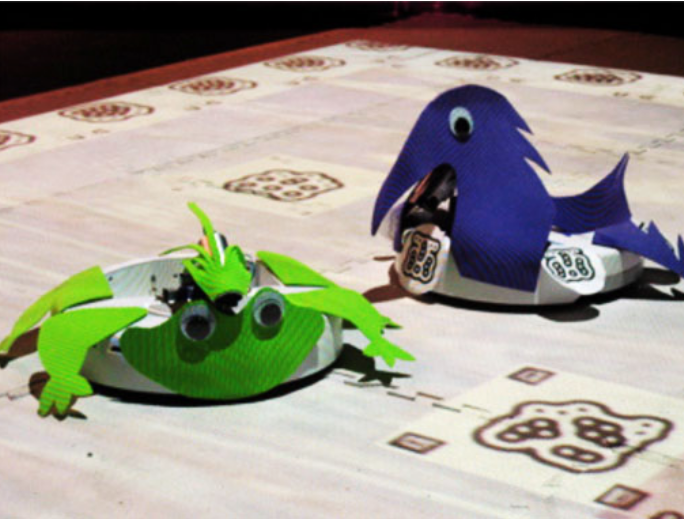
\includegraphics[width=.6\linewidth,fbox]{figs/alert.png}
    \caption{ALERT.}
    \label{fig:alert}
    \source{\citeonline{burleson_active_2018}}
\end{figure}

Com relação à depuração, a programação interativa se apresenta como um diferencial. A execução dos comandos a medida que o brinquedo os detecta, possibilita às crianças corrigirem o algoritmo durante a execução. Os autores exemplificam que se o brinquedo faz um movimento em U, quando o esperado era um giro à direita, as crianças podem adicionar novos comandos na frente dele. Deste modo a criança tem interação constante tanto com o robô quando com o algoritmo, que se torna algo móvel. 

\subsection{Análise Comparativa}

%%%%%%%%%%%%%%%%%
As seções anteriores apresentaram quatro trabalhos relacionados com programação de brinquedos programáveis por crianças. Além disso, todos tem alguma característica relacionada à depuração de algoritmos. Esta seção compara estes trabalhos entre si quanto às seguintes característica: idade do público-alvo, tipo de interface, e depuração (\autoref{quadro:comparision}). Por fim, os trabalhos são posicionados em relação à solução proposta.

Em relação ao público-alvo, o Robo-Blocks foca em crianças de 8 a 9 anos, pois a criança precisa entender basicamente o significado dos algarismos numéricos ao parametrizar o ângulo do giro do robô, e nesta idade as crianças normalmente aprenderam ler \cite{committee_on_the_prevention_of_reading_difficulties_in_young_children_preventing_1998}. Em contrapartida, o Cubetto, a Bee-Bot\footnote{Existem versões com texto nos botões \it{clear}, \it{go} e \it{pause}, mas os botões provocam sempre o mesmo comportamento. Mesmo que não saiba ler, a criança consegue mapear a ação do botão com sua funcionalidade.} e o ALERT não dependem diretamente de números, e por isso consegue atender um público a partir dos 4 ou 6 anos.

Com relação ao tipo de interface, todos os trabalhos utilizam interface tangível, porém seguindo diferentes abordagens. O Robo-Blocks tem blocos eletrônicos, que são encaixados entre si e possuem um display que mostra o tamanho do avanço ou giro. O Cubetto também é programado por blocos tangíveis, porém a parte eletrônica está no painel onde os blocos são encaixados. Isso possivelmente diminui o custo com blocos e centraliza os possíveis problemas eletrônicos no painel. A Bee-Bot, por sua vez, não é programada por blocos, mas sua interface de botões é tangível \cite{}

%Quais são as ações possíveis? Qual o estado atual? Qual o resultado de cada ação?

{{\renewcommand{\arraystretch}{1.5}
    \begin{quadro}[!h]
        \caption{Análise comparativa.}
        \vspace{-15pt}
        \begin{tabularx}{\textwidth}{ @{} | p{.2\linewidth} | p{.1\linewidth} | X | X | @{} }
        \hline
        \textbf{Projeto ou ferramenta}  & \textbf{Idade do público-alvo}  & \textbf{Tipo de interface}       &\textbf{Depuração}                                          \\ \hline
        
        Robo-Blocks                     & 8 a 9 anos                      & Tangível com blocos eletrônicos  & Execução passo a passo, protractor e marcadores de erros   \\ \hline
        Cubetto                         & 4 a 8 anos                      & Tangível com painel eletrônico   & Destaca blocos em execução                                 \\ \hline
        Bee-Bot com mesa interativa     & 4-5 a 12-14 anos                & Tangível com botões              & Mostra caminho percorrido                                  \\ \hline
        ALERT                           & 6 anos                          & Tangível com projeção            & Permite alterar o comportamento do robô durante a execução \\ \hline
        Este trabalho                   & 4 a 6 anos                      & Tangível com projeção            & Destaca blocos em execução                                 \\ \hline
        \end{tabularx}
        \vspace{-10ppt}
        \sourceauthor
        \label{quadro:comparision}
    \end{quadro}

}

Esta pesquisa analisou três classes de trabalhos similares. Primeiramente buscou artigos sobre uso de brinquedos programáveis em atividades com crianças de \idadeinicial a \idadefinal anos, dos quais foram identificados os métodos e aprendizados resultantes. A seguir foi realizado um mapeamento industrial, onde foram analisados 56 brinquedos programáveis construídos por empresas que vendem ou planejam vender esses brinquedos. A terceira classe de trabalhos

.

Esta pesquisa se difere da primeira classe de trabalhos (\autoref{quadroartigosrsl}) quanto à fonte de dados para análise. As pesquisas apresentadas avaliam notas e vídeos. A presente pesquisa pretende coletar automaticamente interações ocorridas com o brinquedo. Outra diferença é que as pesquisas da primeira classe verificaram o impacto de uma ferramenta no aprendizado de aspectos do PC ou compararam duas ferramentas. Este trabalho, por sua vez, compara o mesmo brinquedo em duas situações: estando ou não associado a uma ferramenta de projeção de comandos.

A segunda classe são brinquedos disponíveis comercialmente, nos quais se analisou os tipos de interface, o uso de realidade aumentada e os conceitos de algoritmos abordados. O mapeamento apontou apenas dois brinquedos usando realidade aumentada (o Augie e o Botzees), no modo \textit{window-on-the-world}, por meio de \textit{tablets} e \textit{smartphones}. A realidade aumentada utilizada neste trabalho é o modo projetivo, em que a criança deve interagir com uma interface tangível combinados com objetos virtuais projetados e não deve ter contato com telas sensíveis ao toque.

A terceira classe apresenta quatro tipos de interface. O ARBlocks é uma interface de realidade aumentada; o Go Robot Mouse é um brinquedo tangível programado por botões; o Big Hero: Code Baymax é um jogo de interface gráfica; e o ALERT é uma interface de programação espacial.

Esses trabalhos tem semelhanças e diferenças com esta pesquisa (\autoref{quadro:relacionados}). Quanto às semelhanças, os trabalhos 2, 3 e 4 utilizam alguma forma de representação espacial do algoritmo a ser executado, assim como a presente pesquisa. Os trabalhos 1 e 4 utilizam projeção dos comandos, assim como a ferramenta aqui proposta. Quanto às diferenças, nenhuma das ferramentas possibilita inserir comandos por meio de botões ou de interface tangível. 

Por fim, esse capítulo ressalta três aspectos. (i) O mapeamento industrial não apontou uso de realidade aumentada projetiva com brinquedos programáveis. Entretanto (ii) os trabalhos relacionados demonstram que usar projeção em interfaces de programação é viável e abre novas possibilidades de interação, como a programação espacial descrita por \citeonline{burleson_active_2018}. Além disso, o mapeamento indicou (iii) uso de interfaces tangíveis por 55\% dos brinquedos. A proposta apresentada no \autoref{c_desenvolvimento} considera esses três aspectos e busca representar um tipo inovador de interação, ou, ao menos, contribuir com pesquisas que indiquem a adequação da realidade aumentada projetiva aplicada à interfaces de brinquedos programáveis.

\begin{quadro}[!htbp]
 \begin{longtable}{p{3cm} p{4cm} p{4cm} p{4cm} }
 \hline
 
 Publicação & Tipo de Interface & Vantagens & Desvantagens \\ \hline
 \endhead
 1 - ARBlocks \citeonline{roberto_dynamic_2013} & 
 Tangível projetiva de realidade aumentada. Usuário interage por meio de blocos e o sistema projeta imagens sobre os blocos. & 
 Facilidade em criar aplicações com os mesmos blocos físicos. Atração da atenção dos estudantes. & 
 Necessita de ajuste fino da luminosidade do ambiente. \\ \hline
 
4- ALERT
\citeonline{burleson_active_2018} &
Tangível espacial. Usuário posiciona marcas fiduciais no caminho do robô e ele interpreta e executa. &
Possibilidade de alterar o algoritmo em tempo de execução. Facilidade em criar comandos sem alterar o hardware do brinquedo. &
As marcas fiduciais não tem significado visível ao olhar humano. \\ \hline

Esta pesquisa &
Tangível (botões do brinquedo) projetiva. Usuário interage por meio dos botões do brinquedo e sistema projeta algoritmo no caminho do brinquedo. &
Tangibilidade do meio de inserção (botões) e facilidade em ver o caminho a ser percorrido pelo brinquedo sobre o mapa físico. &
Possível oclusão das marcas fiduciais. Falta de significado das marcas fiduciais para o olhar humano. \\ \hline

 \end{longtable}
 \caption{Trabalhos relacionados.}
 \label{quadro:relacionados}
 \sourceauthor
\end{quadro}

\section{Revisão Sistemática: Pesquisas de IHC com crianças}
\label{sec_rsl}
Para compreender como são feitas as pesquisas sobre brinquedos programáveis com crianças, o método utilizado foi o de revisão sistemática \cite{kitchenham_guidelines_2007}. Esse método é um tipo de estudo secundário, que revisa estudos primários a respeito de uma pergunta de pesquisa, tópico ou fenômeno de interesse. No processo busca-se identificar, avaliar e interpretar as publicações relevantes para o tema em questão, e evitar o viés de quem produziu a pesquisa.

Seguindo a sequência proposta por \citeonline{kitchenham_guidelines_2007}, a primeira etapa identificou a necessidade da revisão. A string de busca 

\textit
{
    (“jardim de infância” OR “educação infantil”) AND (currículo OR atividades) AND (algoritmos OR programação OR computação) AND "\acl{PC}"
}

foi aplicada no GoogleScholar. O resultado da busca foram 551 artigos, o que indicou a necessidade de uma revisão.

\subsection{Questões de Pesquisa}
Três questões exploratórias guiaram a busca:

\begin{itemize}
    \item QE1 - Quais tipos de interfaces são usadas em pesquisas sobre aprendizado de algoritmos na Educação Infantil? 
    \item QE2 - Quais métodos e design de experimentos são utilizados?
    \item QE3 - O que as crianças aprendem ao interagir com brinquedos programáveis?
\end{itemize}

\subsection{Resultados}

Após definir as perguntas de pesquisa, foi definido um protocolo de busca para a execução da revisão sistemática. Foram usadas strings de busca específicas para cada repositório (\autoref{apendice_a}). Sobre os resultados, foram aplicados os critérios de inclusão e exclusão primeiramente sobre os resumos e depois sobre o texto completo (\autoref{quadro_criterios}). Após a aplicação dos critérios 7 artigos restaram.

\begin{quadro}[!htbp]
\caption{Critérios de inclusão e exclusão.}
\label{quadro_criterios}
 \centering
 \begin{tabular}{|p{.45\textwidth}|p{.45\textwidth}|}
 \hline
 Critérios de inclusão & Critérios de exclusão \\ 
    \hline
    
    \begin{minipage}{.45\textwidth}
        1. Estudos primários indicando intervenção relacionada a ensino/aprendizado de algoritmos na Educação Infantil \\ 
        2. Estudos publicados entre 2015 e 2020 \\
        3. Estudos com crianças entre 3 e 6 anos \\
    \end{minipage}
    
    &
    
    \begin{minipage}{.45\textwidth}
    \vspace{.5cm}
        1. Artigos em línguas diferentes de inglês e português \\ 
        2. Título ou resumo mencionando nível diferente de Educação Infantil \\
        3. Foco em formar professores \\
        4. Menos de 5 páginas  \\
        5. Estudos secundários ou terciários \\
        6. Estudos focados em público-alvo diferente desta pesquisa \\
        7. Estudos duplicados \\
        8. Estudo que não aborda criação de algoritmos por crianças \\
        9. Estudo cujo texto completo não foi possível acessar \\
    \end{minipage}

 \\ \hline
 
 \end{tabular}
\end{quadro}

O critério de inclusão 3 (idade entre 3 a 6 anos) filtrou 82 trabalhos, pois grande parte dos estudos tem público-alvo maior de 6 anos. O segundo critério que filtrou mais artigos (CI1) aplicou-se a 30 artigos que não apresentaram nenhum tipo de intervenção com crianças, a fim de mensurar resultados como a qualidade de alguma ferramenta ou aprendizado de algoritmos. Outros 15 trabalhos focaram em públicos específicos que se diferenciam do público desta pesquisa, e portanto foram desconsiderados. O \autoref{quadroartigosrsl} apresenta os artigos que passaram no filtro.

\begin{table}[!htbp]
    \begin{center}
    \begin{footnotesize}
    \caption{Resultados da RSL}
    \label{rsl_table}

    \begin{tabular}{|c|c|c|c|c|c|c|c|c|c|c|} \hline
        Repositório         & Res. & CE1 & CE2 & CE3 & CE4 & CE5 & CE6 & CE7 & CE8 & CE9 \\ \hline
        ERIC                & 4  &  3  &  2 &  2 &  2 &  2 & 2  &  2 &  2 & 2  \\ \hline
        ACM Digital Library & 39 & 33  & 11 & 11 & 10 &  7 & 3  &  3 &  2 & 2  \\ \hline
        Science Direct      &  7 &  7  &  3 &  3 &  3 &  2 & 2  &  2 &  2 & 2  \\ \hline
        IEEE Xplore        & 114 & 91  & 36 & 32 & 32 & 21 & 13 & 11 & 11 & 1  \\ \hline
        Total              & 164 & 134 & 52 & 48 & 47 & 32 & 20 & 18 & 17 & 7  \\ \hline 
        Filtrados          & -   &  30 & 82 &  4 &  1 & 15 & 12 &  2 & 1  & 10 \\ \hline 
    \end{tabular}
    
    \end{footnotesize}
    \end{center}
    \sourceauthor
\end{table}

\begin{landscape}
\linespread{1}
\begin{footnotesize}
\begin{quadro}
 \caption{Artigos resultantes da RSL}
 \label{quadroartigosrsl}
\end{quadro}
\begin{longtable}{|p{6cm}|p{8cm}|p{8cm}|}
    \hline
    
    Publicação & Métodos utilizados / interfaces & Resultados / aprendizados \\ \hline
    
    \endhead
    
    \citeonline{repiso_robotics_2019} \newline
    \textit{Robotics to develop computational thinking in early Childhood Education} &
    
    Intervenção com a Bee-Bot® durante 7 encontros. Pesquisa quantitativa, quasi-experimental, com pré e pós teste. As crianças programaram usando botões e cartas. A avaliação utilizou desafios de programação com histórias lúdicas. As professoras e pesquisadores atribuíram notas de 0 a 5 conforme \citeonline{bers_computational_2014}. &
    
    A intervenção causou resultados positivos no grupo experimental nos aspectos de sequenciamento, correspondência ação-instrução e depuração. \\ \hline
    
    \citeonline{nam_connecting_2019}
    \textit{Connecting Plans to Action: The Effects of a Card-Coded Robotics Curriculum and Activities on Korean Kindergartners} &
    
    Intervenção utilizou a TurtleBot durante 8 encontros de 90 minutos com 53 crianças, uma vez por semana. As crianças planejaram o deslocamento desenhando e programaram usando cartões. Pesquisa quantitativa, quasi-experimental, com pré e pós teste. As professoras participaram da intervenção, auxiliando as crianças. &
    
    Apresentou resultados positivos nas habilidades de sequenciamento e resolução de problemas para o grupo experimental. \\ \hline
    
    \citeonline{di_lieto_educational_2017}
    \textit{
    Educational Robotics intervention on Executive Functions in preschool children: A pilot study
    } &
    
    Intervenção com a Bee-Bot® durante 6 semanas, duas vezes por semana, sendo 75 minutos por sessão. Divisão em grupos de 3 a 4 crianças, cada criança com um robô. Aumento gradual do tamanho do caminho a ser percorrido. Execução de testes de programação e psicológicos (memória, visão espacial e atenção). Uso de pré e pós teste. &
    
    Resultados indicaram aumento da capacidade de atenção e memória de trabalho. Melhoria na habilidade de programação das últimas 3 sessões comparadas às 3 primeiras. \\ \hline
    
    \citeonline{sheehan_parent-child_2019}
    \textit{Parent-child interaction and children's learning from a coding application} &
    
    Pesquisa quantitativa. Em dupla com seus pais, 31 crianças interagiram com o ScratchJr durante 10 minutos. Pesquisadores gravaram e transcreveram as conversas entre pais e filhos. Foram extraídas falas sobre linguagem espacial e perguntas. A linguagem foi relacionada com a produção e compreensão de comandos. &
    
    Os pais utilizaram mais termos de linguagem espacial e fizeram mais perguntas do que seus filhos, para auxiliá-los. O número de perguntas foi um preditor negativo da produção e compreensão de comandos. \\ \hline
    
    \citeonline{pila_learning_2019}
    \textit{Learning to code via tablet applications: An evaluation of Daisy the Dinosaur and Kodable as learning tools for young children} &
    
    Pesquisa qualitativa com pré e pós teste. 28 crianças de 4 a 6 anos usaram, durante uma semana, 2 aplicativos para ensino de programação (Kodable e Daisy the Dinossaur). A pesquisa captou o quanto as crianças gostaram de cada aplicativo e a influência do gênero no desempenho. Também foi avaliada o reconhecimento de comandos antes e após a intervenção, com notas de 0 a 5 conforme \citeonline{bers_computational_2014}. &
    
    Testes t identificaram um aumento significativo no reconhecimento dos comandos do aplicativo Daisy. Após uma semana foi possível identificar compreensão de habilidades gerais de codificação. O “apelo” do aplicativo teve correlação com o aprendizado resultante, e o gênero não afetou o desempenho. \\ \hline
    
    \citeonline{burleson_active_2018}
    \textit{Active Learning Environments with Robotic Tangibles: Children's Physical and Virtual Spatial Programming Experiences} &
    
    Pesquisa qualitativa comparando o uso de duas ferramentas de programação espacial, sendo uma virtual e outra tangível (Robopad e ALERT). 9 crianças de 6 anos, divididas em 4 grupos, interagiram durante 5 dias (num calendário de 2 semanas) com ambas as ferramentas. &
    
    Usando o ALERT as crianças foram capazes de programar, colaborativamente, sequências para alterar o comportamento do robô. A ferramenta Robopad induziu mais a alterar/depurar o “programa” em tempo de execução.  \\ \hline
    
    \citeonline{heljakka_gamified_2019}
    \textit{Gamified Coding: Toy Robots and Playful Learning in Early Education} &
    
    Pesquisa qualitativa. Durante um período de 6 meses os pesquisadores disponibilizaram os brinquedos programáveis Dash e Botley a duas professoras e 21 crianças de 5 anos. As crianças brincaram livremente com os brinquedos e as professoras registraram o quão rápido as crianças aprenderam a programá-los. Os pesquisadores visitaram a sala de aula e entrevistaram crianças e professoras. &
    
    As crianças aprenderam a programar os brinquedos e também criaram brincadeiras, como criar um túnel com as pernas para o Dash passar e construir caminhos para o Botley percorrer. \\ \hline
    
    Esta pesquisa & Pesquisa mista. Coleta automática de interações. Uso do brinquedo RoPE com e sem realidade aumentada. & Pretende-se mensurar a colaboração, a depuração, e o número de erros ligados à lateralidade. \\ \hline
    
    \end{longtable}   
\end{footnotesize}

\end{landscape}

\subsection{QE1 - Quais tipos de interfaces são usadas em pesquisas sobre aprendizado de algoritmos na Educação Infantil? }

O tipo de interface mais citado nos resultados foram brinquedos controlados por botões. A Bee-Bot apareceu em duas pesquisas, e outros brinquedos programados por botões foram a TurtleBot e o Botley. Aplicativos citados foram o ScratchJr, a interface do Dash, o Kodable, e \textit{Daisy the Dinossaur}. Outro tipo de interface citado é a espacial: \citeonline{burleson_active_2018} apresenta o ALERT e o Robopad, em que os agentes se movem no espaço e captam os comandos do ambiente.

Além das interfaces, outra variável a ser considerada são os tipos de atividades realizadas. Uma mesma interface, utilizada de modos diferentes pode gerar diferentes aprendizados. A sequência de atividades do TangibleK Robotics Currículum, desenvolvida por \citeonline{bers_computational_2014} foi aplicada por \citeonline{repiso_robotics_2019} e por \citeonline{pila_learning_2019}. Dividida em 7 encontros, o primeiro dia de atividades iniciou com a exploração da interface da Bee-Bot, seguida (nos dias 2 e 3) da programação do brinquedo para se deslocar sobre tapetes. Nos dias 4 e 5 foram introduzidas cartas correspondentes às instruções, para serem sequenciadas e depois comparadas com os movimentos do brinquedo. Nos dias 6 e 7 foram mostradas sequências de comandos com erros, e as crianças exercitaram a depuração ao encontrar esses erros.

\citeonline{di_lieto_educational_2017} apresenta atividades de dificuldade incremental, em que as crianças precisavem programar a Bee-Bot para se deslocar sobre um tapete de formas cada vez mais complexas. \citeonline{heljakka_gamified_2019} não definiram nenhuma atividade específica para as crianças, apenas permitiram a exploração dos brinquedos Botley e Dash por 6 meses.

\subsection{QE2 - Quais métodos e design de experimentos são utilizados?}

O método mais utilizado foi a pesquisa quasi-experimental, com pré e pós teste. Das 7 pesquisas, 4 foram quantitativas, 2 qualitativas e uma mista. Além disso, \citeonline{nam_connecting_2019} e \citeonline{repiso_robotics_2019} utilizaram grupo de controle e experimental.

O tempo das intervenções variou consideravelmente. As pesquisas objetivando mensurar efeitos decorrentes das interações com os brinquedos foram mais longas, durando de 7 encontros a 6 meses. A pesquisa que buscou avaliar a usabilidade foram mais rápidas, durando 10 minutos.

As amostras utilizadas foram de conveniência, com experimentos realizados nos ambientes escolares. O tamanho das amostras variou entre 9 e 31 crianças, que em trabalharam em grupos em 6 das 7 pesquisas. As fontes de dados utilizadas foram vídeos, mapa de eventos, rubricas, transcrições e entrevistas. 

\subsection{QE3 - O que as crianças aprendem ao interagir com brinquedos programáveis?}

Os trabalhos citam principalmente o aprendizado de sequenciamento e de algoritmos em geral. \citeonline{pila_learning_2019}, após a interação de um conjunto de crianças durante 5 dias com os aplicativos Daisy e Kodable, perguntaram às crianças “O que é programar?”. A nota máxima foi dada a respostas que apresentavam a ideia de causa e efeito aplicável à tecnologia em geral, por exemplo “programar é colocar código em algo para que faça alguma ação”. Os resultados indicaram que as crianças não evoluíram na capacidade de expressar verbalmente seu entendimento de codificação.

Um outro aspecto da compreensão algorítmica avaliado por \citeonline{repiso_robotics_2019} e \citeonline{pila_learning_2019} é a compreensão dos símbolos da interface. \citeonline{repiso_robotics_2019} investigaram a compreensão sobre a correspondência entre ação e instrução, que significa relacionar qual ação o robô executa em correspondência a um símbolo da instrução. A partir das rubricas os pesquisadores identificaram uma evolução significativa no grupo experimental. \citeonline{pila_learning_2019} mostrou quatro símbolos da interface do aplicativo Daisy para as criaças e solicitou que explicassem verbalmente o significado do símbolo. No pré-teste a média de acerto foi de 0.5 e no pós-teste esse valor subiu para 2.3.

\citeonline{nam_connecting_2019} avançaram nessa compreensão e utilizaram um instrumento para captar a compreensão de sequências. O instrumento utilizado solicita que crianças organizem 4 imagens que mostram eventos sequenciais, dada a imagem inicial. Os resultados apontaram evolução significativa na pontuação de sequenciamento para o grupo experimental.

\section{Mapeamento Industrial: Interfaces de Brinquedos Programáveis}
\label{secao_mapeamento_industrial}

O mapeamento industrial buscou encontrar o maior número possível de brinquedos programáveis que estão ou estiveram disponíveis para comercialização\footnote{O mapeamento fez parte de uma pesquisa voltada a brinquedos com características inteligentes, como IA e IoT. Nesta seção os dados serão avaliados com foco em realidade aumentada.}. A busca por estas fontes se justifica por abranger empresas e produtos que não estão diretamente ligados a publicações acadêmicas. Portanto, a pesquisa não utilizou bases científicas, mas sim plataformas de comércio eletrônico e buscadores. O mapeamento seguiu três etapas \cite{cooper_alice:_2000}:
\begin{enumerate}
    \item Definição das questões de pesquisa
    \item Planejamento do processo de busca
    \item Definição dos critérios para filtrar os resultados
\end{enumerate}

As próximas subseções detalham essas etapas da forma mais transparente possível.

\subsection{Questões de Pesquisa}

Três questões exploratórias guiaram o processo de busca:

\begin{enumerate}
    \item Quais são os tipos de interfaces mais frequentemente utilizados em brinquedos programáveis?
    \item Como a realidade aumentada é aplicadas em brinquedos programáveis?
    \item Quais são os conceitos de algoritmos abordados? 
\end{enumerate}

\subsection{Processo de Busca}
A segunda etapa define a \textit{string} de busca a ser aplicada em campos de pesquisa. O foco esteve em programação, resultando na seguinte \textit{string}:

\textit{ ((coding OR programmable) AND toys) }.

Seguindo a estratégia também apresentada no mapeamento feito por \citeonline{kitchenham_guidelines_2007}, uma exploração inicial indicou o uso das seguintes fontes de busca:

\begin{itemize}
    \item Plataforma de comércio eletrônico Amazon.com
    \item Postagens de blogs encontrados em pesquisas no Google e no DuckDuckGo
    \item Plataforma de financiamento coletivo Kickstarter.com
    \item Vídeos do Youtube
\end{itemize}

Além destas fontes, um lista de páginas online selecionadas pelo orientador desta pesquisa durante estudos sobre o tema contribuiu como fonte de busca.

A string de busca foi aplicada nos sites que oferecem campos de pesquisa. Outra fonte de busca foram as categorizações de produtos existentes nos websites. O site kickstarter.com, por exemplo, tem uma área específica sobre projetos de robótica, enquanto plataforma amazon.com possui uma categoria de produtos denominada \textit{coding toys}. Essas categorizações foram consultadas e os resultados adicionados aos resultados da busca textual. Por fim, a abrangência do mapeamento foi validada por meio da consulta artigos de revisão a fim de encontrar brinquedos faltantes. Os artigos consultados foram o de \cite{} Nesta etapa 5 brinquedos foram adicionados.

\subsection{Filtro}
Os critérios de inclusão foram três. Primeiramente, a presença de alguma forma de inserir comandos a serem executados pelo brinquedo. O segundo critério é a presença de algum componente tangível, ou seja, aplicativos sem interação com brinquedo físico foram descartados. O último critério é a presença de algum componente eletrônico, de forma que a haver um processamento dos comandos programados para controlar sua execução. Esse critério eliminou os jogos de tabuleiro e livros de programação \cite{hamilton_emerging_2020}.

Após encontrar brinquedos adequados aos critérios de inclusão, a próxima etapa foi obter dados sobre as interfaces de programação. Para cada brinquedo foi executada uma pesquisa por vídeos demonstrando o uso do brinquedo. Outras fontes de dados foram as descrições presentes nas páginas de comércio eletrônico e páginas dos fabricantes. 

\subsection{Resultados}
Um total de 86 brinquedos resultaram do processo de busca. Destes, 56 serviram como objeto de análise para responder as três perguntas de pesquisa. Os outros 30 brinquedos não foram analisados por terem sido adicionados à lista posteriormente ou por serem versões similares de algum dos brinquedos analisados. Os resultados estão disponíveis no endereço \url{https://bit.ly/35cUbZ1}. O \autoref{quadro:toys_reviewed} sumariza os brinquedos utilizados na análise.
\begin{landscape}
\linespread{1}
\begin{quadro}
 \caption{Brinquedos resultantes do mapeamento industrial.}
 \label{quadro:toys_reviewed}
\end{quadro}
\begin{small}
\begin{longtable}{|p{4.5cm} p{4.5cm} r| p{4.5cm} p{4.5cm} r|}
    \hline
    Nome & Fabricante & Ano & Nome & Fabricante & Ano \\ \hline
    Big Trak / Big Track Junior & Milton Bradley & 1979 &
    Sphero SPRK+ & Sphero & 2016 \\ \hline
    Topobo & MIT Tangible Media Group & 2003 &
    Go Robot Mouse & Learning Resources & 2016 \\ \hline
    Finch & BirdBrain Technologies & 2010 &
    Coji & WowWee & 2016 \\ \hline
    Bee-Bot & TTS Group & 2011 &
    KUMIITA & ICON Corp & 2016 \\ \hline
    KIBO & Kinderlab Robotics & 2012 &
    RoPE & SmartFun Brasil & 2017 \\ \hline
    Dr. Wagon & Stanford & 2012 &
    Harry Potter Coding Kit & KANO & 2017 \\ \hline
    Ollie & Sphero & 2012 &
    Meccano-Erector Meccanoid & Spin Master & 2017 \\ \hline
    RoboTami Creative Robot Kit & Robotron & 2012 &
    Lego Boost & Lego & 2017 \\ \hline
    Lego Mindistorms EV3 & Lego & 2013 &
    Anki Cozmo & Digital Dreams & 2017 \\ \hline
    Romo & Romotive & 2013 &
    Sam Curious Cars Kit & Sam Labs & 2017 \\ \hline
    Pro-Bot & TTS Group & 2014 &
    Airblock & Makeblock & 2017 \\ \hline
    Dot & MakeWonder & 2014 &
    Augie & Pai Technology & 2017 \\ \hline
    Dash & MakeWonder & 2014 &
    Minion Mip & WowWee & 2017 \\ \hline
    Edison & Edison & 2014 &
    Miko 2 & Miko & 2018 \\ \hline
    Ozobot & Ozobot & 2014 &
    Kids First Coding e Robotics & GIGO & 2018 \\ \hline
    TinkerBots & TinkerBots & 2014 &
    Botley & Learning Resources & 2018 \\ \hline
    TiddlyBot & Agilic & 2014 &
    Q-Scout & RoboBloq & 2018 \\ \hline
    Guimo & Guimo Toys & 2015 &
    InO-Bot & TTS Group & 2018 \\ \hline
    BlueBot & TTS Group & 2015 &
    Codey Rocky & Makeblock & 2018 \\ \hline
    Osmo Coding & Tangible Play Inc & 2015 &
    Aibo - ERS-1000 & Sony & 2018 \\ \hline
    Cubetto & PrimoToys & 2015 &
    Root & iRobot & 2018 \\ \hline
    Cue & MakeWonder & 2015 &
    Rugged Robot & TTS Group & 2019 \\ \hline
    Vortex & DFRobots & 2015 &
    Aukfa / JDBaby / HBuds & Aukfa & 2019 \\ \hline
    mBot & Makeblock & 2015 &
    Qobo & Robobloq & 2019 \\ \hline
    Robotiky & Robotiky & 2015 &
    mTity & Makeblock & 2019 \\ \hline
    SmartiBot & The Crafty Robot & 2015 &
    Botzees & Pai Technology & 2019 \\ \hline
    Robo Wunderkind & Robo Wunderkind & 2015 &
    Mojobot & Project Lab & 2019 \\ \hline
    Code a Pillar / Codipédia & Fisher Price - Mattel & 2016 &
    Mochi & Mochi & 2019 \\ \hline
\end{longtable}
\end{small}
\end{landscape}

Quanto ao ano de lançamento, mais de 80\% dos brinquedos foi lançado depois de 2014, o que corresponde ao crescimento do interesse pelo assunto \acl{PC}. A \autoref{toys_year} demonstra o número de brinquedos lançados por ano, e, comparado com a \autoref{pc_interest}, percebe-se uma semelhança no crescimento e no período de aumento. Isso sugere que os brinquedos estão sendo lançados comercialmente em resposta à uma demanda no campo educacional.

\begin{figure}[!htbp]
    \centering
    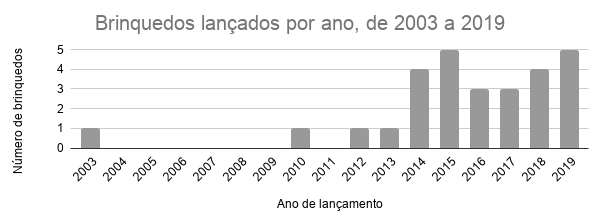
\includegraphics[width=.8\linewidth,fbox]{figs/brinquedos_ano.png}
    \caption{Brinquedos lançados por ano entre 2003 e 2019.}
    \label{toys_year}
    \sourceauthor
\end{figure}

\begin{figure}[!htbp]
    \centering
    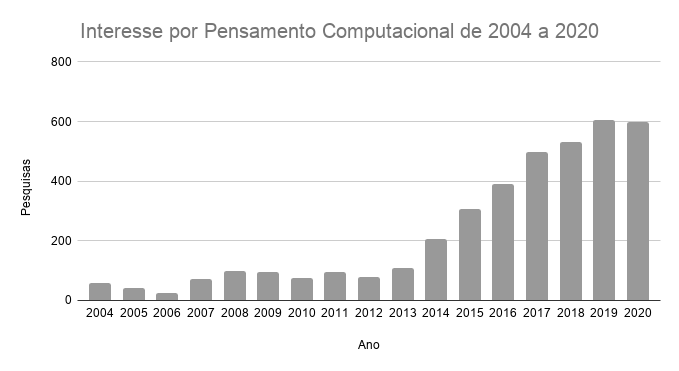
\includegraphics[width=.8\linewidth,fbox]{figs/pc_interest.png}
    \caption{Interesse pelo tema \acl{PC}, segundo o Google Trends.}
    \label{pc_interest}
    \sourceauthor
\end{figure}

\subsection{QE1 - Quais são os tipos de interfaces mais frequentemente utilizados em brinquedos programáveis?}

A resposta a pergunta \textit{QE1 - Quais são os tipos de interfaces mais frequentemente utilizados em brinquedos programáveis?} depende da perspectiva de análise dessas interfaces. Uma pesquisa pode observer os materiais utilizados, enquanto outra observar as cores e formas. O método utilizado para definir essa perspectiva foi o de Kawakita Jiro \citeonline{scupin_kj_1997}. Esse método busca organizar imagens em grupos em três fases: captura, agrupamento e categorização. Ao final é formado um diagrama de afinidades (\autoref{kj}).

\begin{figure}[!htbp]
    \centering
    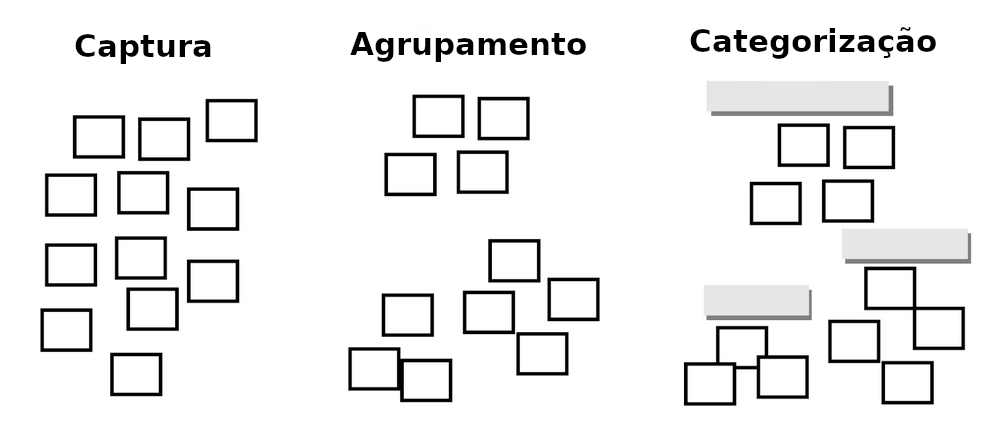
\includegraphics[width=.6\linewidth,fbox]{figs/kj.png}
    \caption{Método Kawakita Jiro.}
    \label{kj}
    \sourceauthor
\end{figure}
Na fase de captura, foram produzidos recortes de imagens focando nas interfaces dos brinquedos de programar. Essas imagens foram obtidas ao parar vídeos de demonstração dos brinquedos. Após a captura, imagens foram distribuídas em um software online e agrupadas por dois pesquisadores. Possíveis divergências, por exemplo, se blocos com texto e ícones pertencem a uma mesma categoria, foram discutidas e sanadas (\autoref{kj_run}).

\begin{figure}
    \centering
    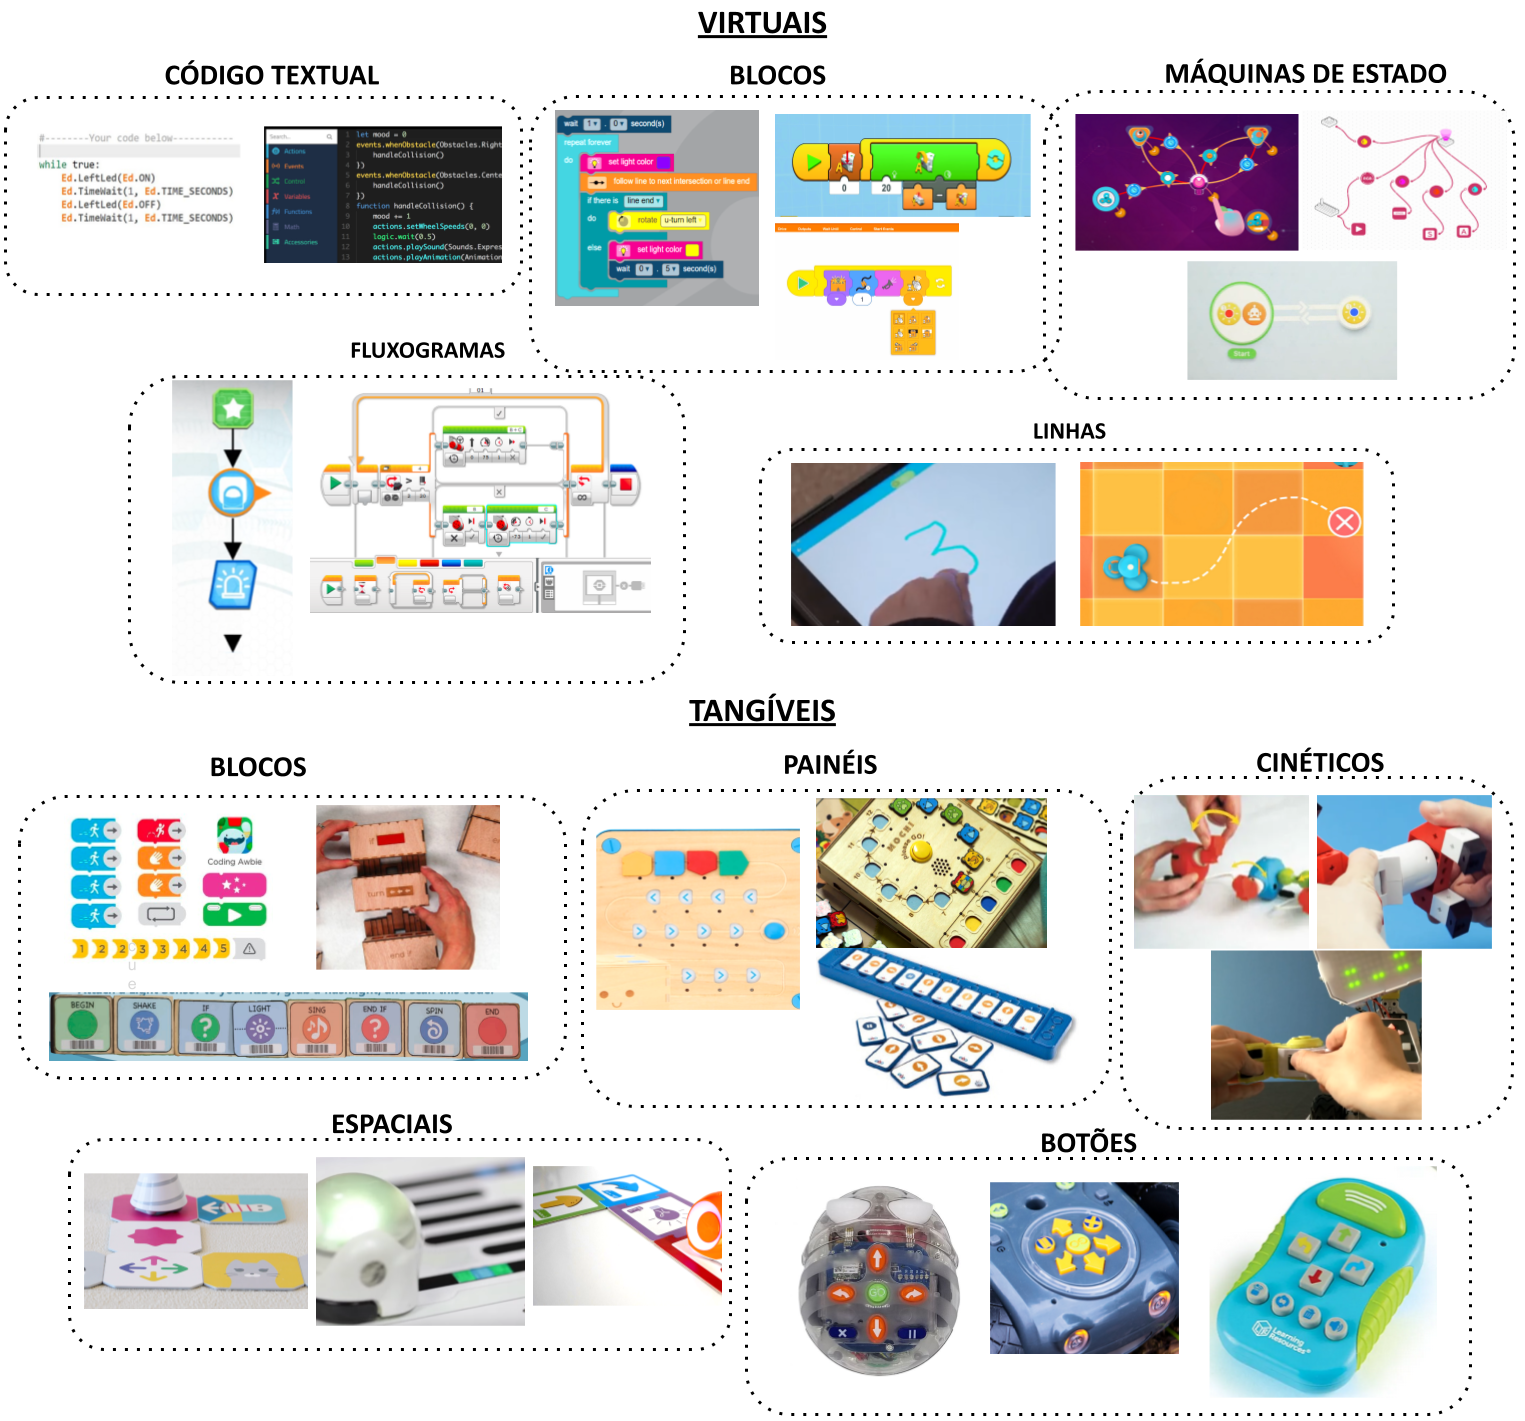
\includegraphics[width=1\linewidth,fbox]{figs/toys_interfaces.png}
    \caption{Agrupamento das interfaces.}
    \label{kj_run}
\end{figure}

O processo resultou em 2 categorias, cada uma com 5 subcategorias. A primeira categoria são as interfaces virtuais, onde há presença de uma tela bidimensional onde os comandos aparecem. A segunda categoria são as interfaces tangíveis, em que a interação ocorre com objetos físicos, como blocos de encaixar ou botões acoplados no brinquedo.

As subcategorias elencadas das interfaces virtuais foram: 
\begin{description}
    \item[Código textual: ] Interfaces que usam código digitado em teclados, como as linguagens de propósito geral. 
    \item[Blocos virtuais: ] Peças de quebra-cabeça que são conectadas e representam estruturas de programação.
    \item[Máquinas de estado: ] Formas geométricas conectadas por linhas, em que cada forma agrupa ações do brinquedo. As linhas representam eventos que provocam a transição entre os estados.
    \item[Linhas: ] Uma linha é desenhada na tela do dispositivo e o brinquedo se move conforme o seu formato.
    \item[Fluxogramas: ] Formas geométricas conectadas por linhas. Cada forma representa uma ação ou uma decisão.
\end{description}

As subcategorias de interface tangível são semelhantes.

\begin{description}
    \item[Blocos físicos: ] Blocos físicos que podem ser interconectados e não precisam ser fixados a um painel. Exemplos: Code a Pillar e KIBO. 
    \item[Painéis: ] Placas de madeira ou de plástico com furos para encaixe de blocos de programação. Exemplos: Cubetto e Mojobot.
    \item[Cinéticos: ] Brinquedos que repetem os movimentos feitos em partes do corpo do brinquedo. Exemplo: Topobo.
    \item[Espacial: ] Brinquedo lê comandos do ambiente usando sensores.
    \item[Botões: ] Botões físicos acoplados ao corpo do brinquedo ou em um controle remoto.
\end{description}

Considerando essa taxonomia, o tipo mais comum de interface de brinquedos programáveis são os blocos virtuais, usada por 30 brinquedos. O segundo tipo mais usado são os botões. Outra tendência observada é o uso de mais de um tipo de interface pelo mesmo brinquedo, a fim de atender um público mais amplo quanto à faixa etária. A \autoref{toys_per_interface_type} descreve o uso de cada um dos tipos de interface.

\begin{figure}[!htbp]
    \centering
    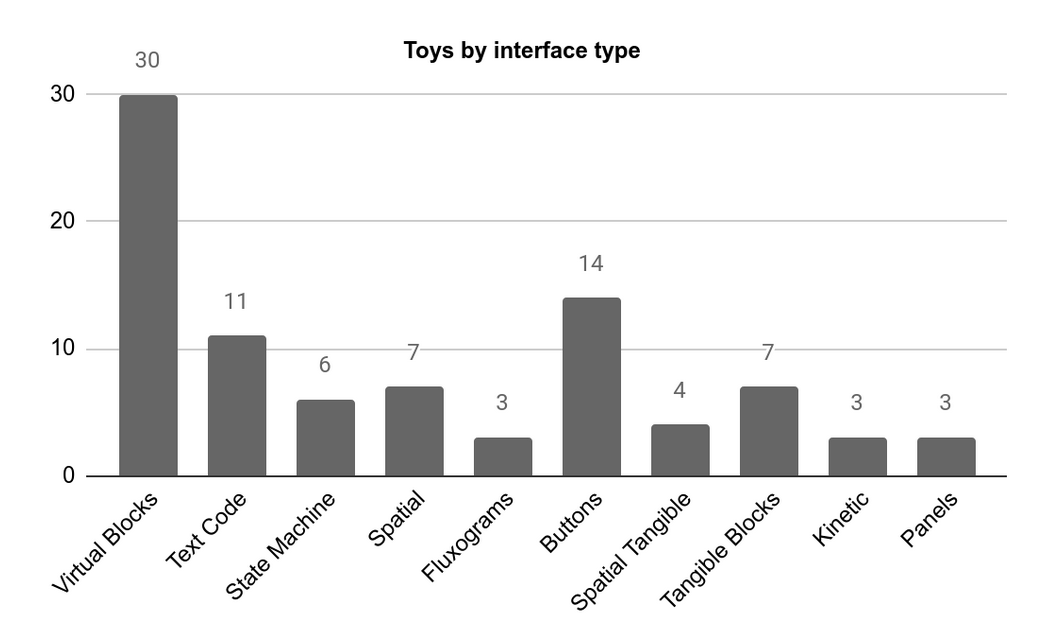
\includegraphics[width=.6\linewidth,fbox]{figs/toys_per_interface_type.png}
    \caption{Brinquedos por tipo de interface.}
    \label{toys_per_interface_type}
    \sourceauthor
\end{figure}

\subsection{QE2 - Como a realidade aumentada é aplicadas em brinquedos programáveis?}
A \ac{RA}, no sentido de combinar objetos virtuais e físicos, é pouco usada em brinquedos programáveis. Dos 56 brinquedos encontrados, apenas 2 seguem essa abordagem: o Botzees e o Augie. Ambos os brinquedos são da empresa \textit{Pai Technology}, a qual apresenta o uso de \ac{RA} como um diferencial da marca.

O tipo de RA utilizado é o \textit{window-on-the-world}, ou seja, um \textit{tablet} ou \textit{smartphone} captura a imagem do brinquedo e associa objetos virtuais à imagem real na tela. No caso do Augie, o brinquedo é captado pela câmera e, ao ter sua posição identificada, personagens aparecem na tela simulando uma batalha com o brinquedo físico. A RA também é usada para mostrar um mapa virtual na tela do \textit{tablet}, e o brinquedo físico percorre esse mapa (\autoref{augie_ar_programming}). O mesmo princípio se aplica ao Botzees. O \textit{smartphone} capta a imagem do brinquedo e mostra a imagem deste ao lado dos blocos virtuais (\autoref{botzees_ar_programming}).

Uma vantagem possível dessa abordagem é a proximidade com que o brinquedo físico e os blocos virtuais aparecem na tela. Isso diminui a necessidade de olhar para dois lugares ao mesmo tempo, ou seja, olhar para a tela do aplicativo e para o ambiente real. Porém não foram encontrados estudos que evidenciem benefícios deste tipo de interface para o aprendizado de programação por crianças. 

\begin{figure}[!htbp]
    \centering
    \begin{subfigure}{.44\textwidth}
        \centering
        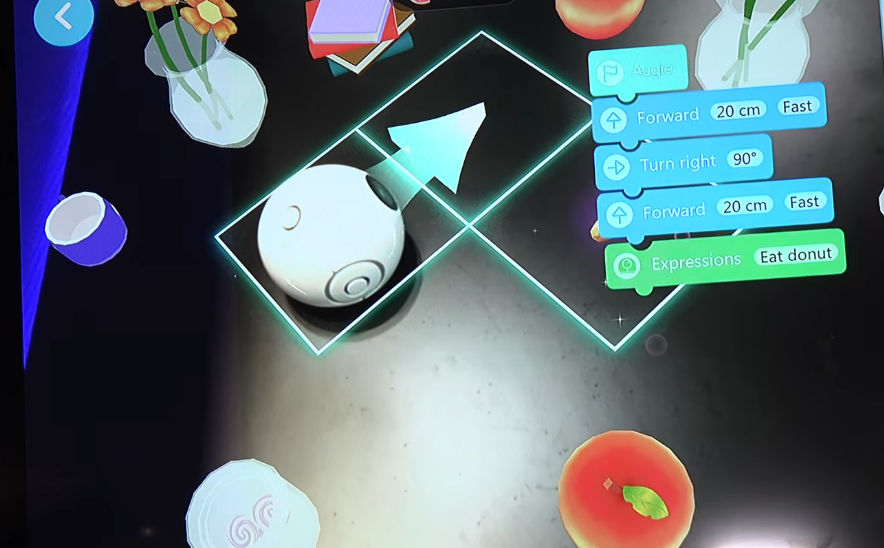
\includegraphics[width=.9\linewidth,fbox]{figs/augie_ar_programming_2.png}
        \caption{Programação do Augie com RA}
        \label{augie_ar_programming}
    \end{subfigure}%
    \begin{subfigure}{.55\textwidth}
        \centering
        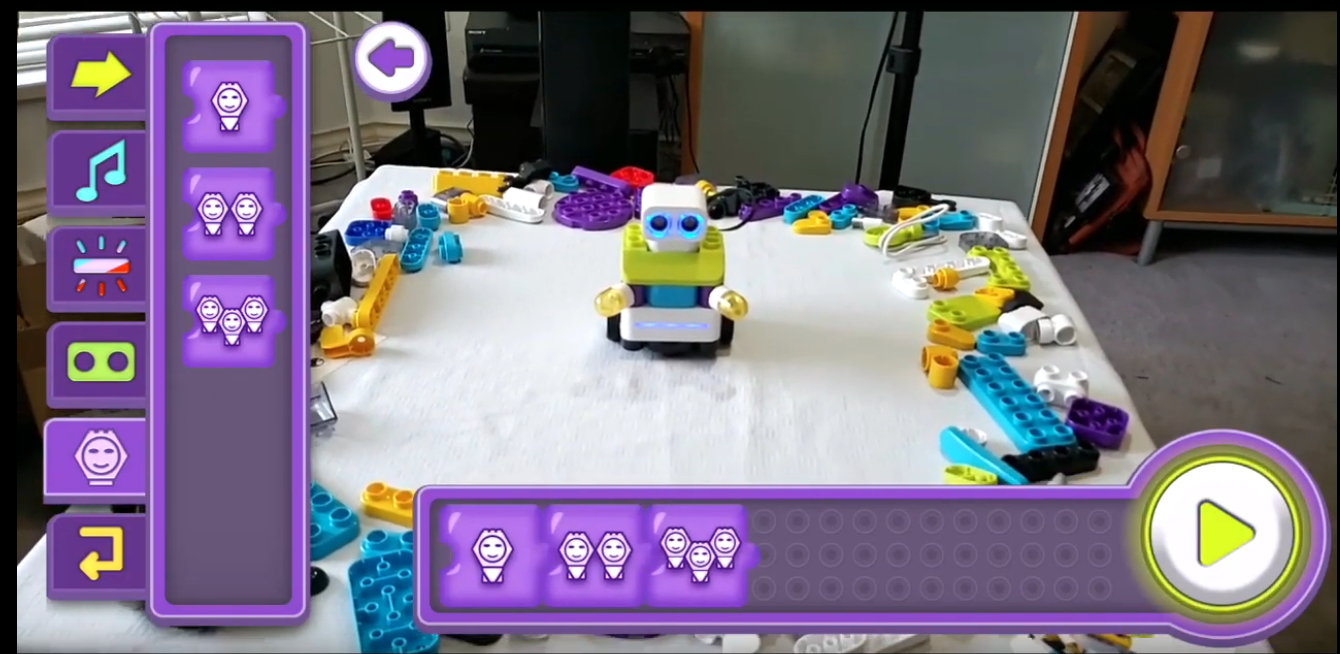
\includegraphics[width=.9\linewidth,fbox]{figs/botzees.png}
        \caption{Programação do Botzees com RA}
        \label{botzees_ar_programming}
    \end{subfigure}
    \caption{Usos de RA com brinquedos programáveis.}
    \label{ar_programming}
\end{figure}

\subsection{QE3 - Quais são os conceitos de algoritmos abordados nas interfaces de brinquedos programáveis?}

A abrangência de conceitos de algoritmos abordados por brinquedos programáveis foi analisada nos seguintes conceitos: variáveis, estruturas de repetição, condicionais, listas, recursividade, paralelismo, sequenciamento, funções, parâmetros e eventos. Aspectos como tipos de dados, constantes, orientação a objetos não foram abordados pois são abstraídos na maioria das interfaces.

\begin{figure}[!htbp]
    \centering
    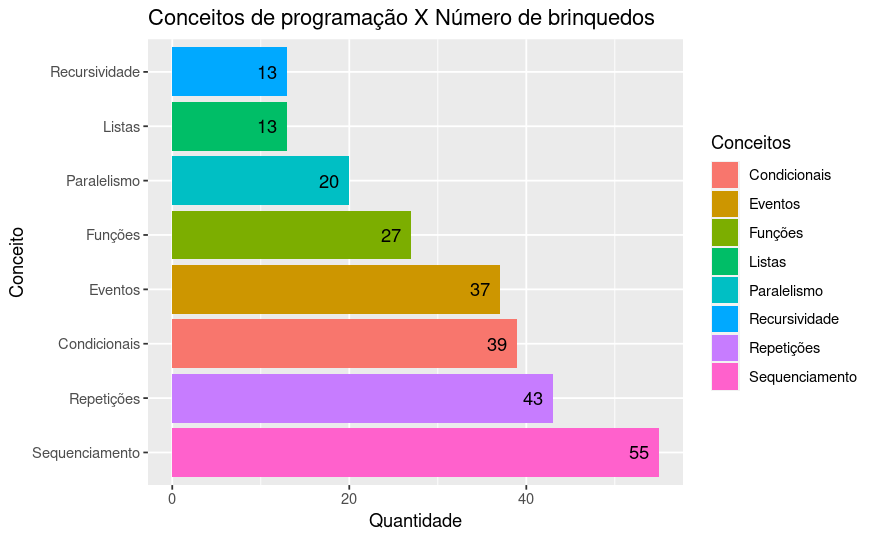
\includegraphics[width=.7\linewidth,fbox]{figs/conceitos_brinquedos.png}
    \caption{Conceitos de programação abordados por brinquedos programáveis.}
    \label{fig:toys_concepts}
    \sourceauthor
\end{figure}

A \autoref{fig:toys_concepts} apresenta o resultado da análise. Como o esperado, o sequenciamento é o conceito mais abordado: criar sequências de comandos a serem executados é intrínseco dos brinquedos programáveis. O segundo conceito mais abordado são repetições, por 76\% dos brinquedos. As estruturas de repetição são normalmente suportadas em interfaces virtuais de programação em blocos. 

Outros dois conceitos interligados são condicionais e eventos. 66\% dos brinquedos disparam algum tipo de evento captado por sensores de luminosidade, proximidade, sons, etc. Esses eventos são usados em condicionais para ações do tipo "se obstáculo à frente", "se luminosidade maior que", entre outros.

Conceitos mais avançados, como paralelismo, recursividade e vetores são suportados pelos brinquedos que tem interfaces de código textual, com suporte a linguagens de propósito geral. Recursividade e vetores são conceitos suportados por 23\% dos brinquedos.

%\section{Comparação dos Trabalhos Relacionados}
%\label{s_c3_comparacao}

%Nesta seção, apresente a análise comparativa dos trabalhos selecionados caracterizando-os em um quadro (conforme exemplificado no \autoref{q_c3-trabalhos}) e posicionando o seu trabalho em relação a eles (na última coluna). Dependendo da quantidade de trabalhos analisados, pode ser necessário elaborar mais de um quadro ou definir uma seção com página no formato paisagem.

%Mesmo que você ainda não tenha apresentado os resultados da sua dissertação no texto, isso conduzirá o restante da leitura, permitindo que você indique a contribuição de cada um dos trabalhos para a solução do problema de pesquisa da sua dissertação e evidencie a sua contribuição, e o diferencial do seu trabalho em relação aos demais. Isso deve ser feito por meio de um texto de discussão apoiado pelos dados apresentados no quadro.

\section{
\chapter{Desenvolvimento}
\label{c_desenvolvimento}

Este capítulo apresenta a interface desenvolvida, denominada de RoPE AR. Primeiramente a \autoref{sec:elementos_interface} descreve a interface do ponto de vista do usuário, ou seja, os elementos com os quais a criança ou o adulto interagem. A seguir a \autoref{sec:detalhes_tecnicos} traz detalhes técnicos das tecnologias utilizadas, como a comunicação Bluetooth entre smartphone e robô.

\section{Elementos da interface}
\label{sec:elementos_interface}
\subsection{Aplicativo}
A interação inicial ocorre quando um adulto usa o aplicativo para conectar o smartphone com o RoPE. Ele é constituído de apenas duas telas. A primeira tela permite conectar o smartphone ao brinquedo (\autoref{fig:app_connection}). Ela mostra um desenho do RoPE e uma lupa indicando a procura pelo brinquedo, ou seja, a conexão com o brinquedo físico. Gravações de uma voz guiam o usuário para que ligue o RoPE acionando seu botão inferior e informam quando a conexão foi estabelecida. Ao se conectar o brinquedo também emite um \textit{feedback} sonoro e luminoso como \i{feedback}.

\begin{figure}[!h]
    \begin{subfigure}{.5\textwidth}
        \centering
        \includegraphics[width=.9\linewidth,fbox]{figs/app_connection.jpeg}
        \caption{Tela de conexão.}
        \label{fig:app_connection}
    \end{subfigure}
    \begin{subfigure}{.5\textwidth}
        \centering
        \includegraphics[width=.9\linewidth,fbox]{figs/app_game.jpeg}
        \caption{Tela de desafio.}
        \label{fig:app_game}
    \end{subfigure}
    \caption{Telas do aplicativo.}
    \label{fig:app_screens}
\end{figure}

A segunda tela aparece após a conexão com o brinquedo. Ela apresenta um desafio contendo uma sequência de mapas (\autoref{fig:app_game}). Cada mapa tem um caminho, uma posição inicial (circulo verde) e um ou mais itens coletáveis. Na direita da tela há um retângulo branco. Ao ser projetada, a cor branca não interfere nas características visuais dos blocos físicos. Manter essas características auxilia na identificação das marcas fiduciais. Por fim, o último elemento da tela são círculos vermelhos que indicam quais blocos fazem parte do algoritmo a ser executado pelo brinquedo. 

Relembrando, a criança não interage com o aplicativo. Toda interação ocorre com o RoPE e com blocos físicos, posicionados no chão. A criança cria algoritmos ao sequenciar os blocos físicos, que são identificados pelo App. Caso exista um algoritmo válido, a luz emitida pelo projetor destaca os blocos do algoritmo.

O brinquedo executa o algoritmo quando a criança pressiona seu botão verde. Ao executar o programa, o brinquedo se move e o aplicativo capta as posições percorridas. Deste modo, consegue identificar se o brinquedo colidiu ou não nos itens coletáveis do mapa. Quando o brinquedo coleta todos os itens, o aplicativo reproduz uma gravação de parabenização, e mostra o mapa seguinte. Caso não existam outros mapas, uma gravação sinaliza que a brincadeira acabou.

\subsection{Elementos tangíveis}
A interface possui quatro tipos de elementos tangíveis: o brinquedo RoPE, os blocos de código, os marcadores de calibragem, e o ativador de depuração  (\autoref{fig:tangible_elements}).
\begin{enumerate}
\item \textbf{Brinquedo RoPE}: Ao brinquedo foi adicionada uma marca fiducial para que seja identificada sua posição. A informação da posição do brinquedo permite à interface reagir a seus movimentos, disparando eventos sonoros e animações. Além da marca fiducial, o brinquedo tem os botões superiores. Por meio do botão verde do brinquedo a criança inicia a execução do algoritmo programado com os blocos de papelão. Os demais botões são usados no modo de depuração. Neste modo, o brinquedo para antes de cada movimento e acende a seta indicando qual será a próxima ação. O brinquedo continua a execução quando o botão é clicado, e assim a criança pode observar a execução passo a passo.
\item \textbf{Blocos de código}:  Há dois tipos de blocos: os direcionais e o bloco de início. Os blocos direcionais tem desenhos que mostram o RoPE fazendo o movimento de andar pra frente, andar para trás, virar a esquerda, e virar à direita. Há também o bloco de início, que corresponde ao botão verde do RoPE e indica o início da execução. Os blocos direcionais devem ser encaixados no bloco de início, formando uma sequência. O formato curvado busca sugerir como deve ser o encaixe entre os blocos. O bloco de início  tem a parte inferior reta para impedir o encaixe de outros blocos incorretamente.
\item \textbf{Marcadores de calibragem}: Marcas fiduciais que identificam os quatro cantos da área projetada. Para projetar os elementos na posição correta o algoritmo precisa mapear a posição de projeção, bem como identificar a distorção de perspectiva resultante. Um adulto responsável por preparar a interface coloca os marcadores nos cantos da área projetada, e a câmera do \textit{smartphone} capta a posição da mesma. Após a captação os marcadores são retirados.
\item \textbf{Ativador de depuração}: O quarto elemento tangível é representado por uma joaninha (em inglês \textit{ladybug}. Essa figura foi selecionada por ser uma figura lúdica e também por ser um inseto, uma referência à origem do termo \textit{bug}. Quando a joaninha está visível o brinquedo RoPE entra em modo de depuração, no qual a execução de cada comando exige que a criança aperte o botão correspondente. Quando não está visível, o brinquedo executa a sequência completa de comandos sem interrupção.
\end{enumerate}

\begin{figure}
\centering
        \includegraphics[width=.9\linewidth,fbox]{figs/tangible_elements.png}
        \caption{Elementos tangíveis. 1 - RoPE. 2 - Blocos de código. 3 - Marcadores de calibragem. 4 - Ativador de depuração.}
        \label{fig:tangible_elements}
\end{figure}
Todos os elementos tangíveis possuem marcas fiduciais de 4cm de diâmetro. Essa medida foi utilizada para facilitar a identificação das mesmas por uma câmera capaz que gera imagens de 1280x720 pixeis durante gravação de vídeo. Essa medida foi obtida de forma empírica, iniciando com 3 cm de diâmetro e aumentando o tamanho até a identificação de todas as marcas presentes no campo de visão da câmera. Um último detalhe é que as marcas são impressas em papel cartão pois este não reflete luz, o que prejudica a captação das marcas.

\section{Aspectos técnicos}
\label{sec:detalhes_tecnicos}
\subsection{Arquitetura}
A arquitetura do projeto possui quatro dispositivos: um smartphone, o brinquedo RoPE, um servidor web e um projetor (\autoref{fig:system_overview}). Estes dispositivos se comunicam por meio de conexão sem fio. Nesta comunicação os dados enviados são as ações executadas pelo brinquedo e as imagens a serem mostradas no tapete.  A seções seguintes apresentam cada um destes componentes.

\begin{figure}[!h]
    \centering
    \includegraphics[width=.8\linewidth,fbox]{figs/system_overview.png}
    \caption{Visão geral dos componentes do sistema.}
    \label{fig:system_overview}
\end{figure}

\subsubsection{Smartphone}
Um smartphone com sistema operacional Android é o componente central, pois coordena a comunicação com o projetor e o servidor web. Dois aplicativos permanecem ativos no smartphone. O primeiro aplicativo é o Mirroring 360, que transmite a tela do smartphone ao projetor via Wi-Fi. Esse aplicativo está disponível na loja de aplicativos da Google, e há diversos aplicativos similares que executam a mesma função. O Mirroring 360 foi selecionado por ser gratuito e não mostrar anúncios.

O segundo aplicativo foi desenvolvido neste trabalho. Ele tem as funções de:
\begin{itemize}
    \item gerar o cenário virtual
    \item captar os blocos tangíveis e, se houver um algoritmo, enviá-lo ao RoPE
    \item detectar colisões entre o RoPE e os elementos virtuais coletáveis
    \item enviar os eventos ocorridos para a CtPuzzle Platform
\end{itemize}

Para isso, o aplicativo é dividido em cinco módulos: Câmera, Detecção de blocos, Análise dos blocos, Registro de interações, e Comunicação com o RoPE . As próximas seções seções apresentam detalhes de implementação destes módulos.

%\begin{figure}
%    \centering
%    \includegraphics[width=0.95\textwidth,fbox]{figs/sequence_diagram.png}
%    \caption{Diagrama de sequência: obtenção de imagem, identificação dos topcodes e análise dos elementos tangíveis.}
%    \label{fig:sequence_diagram}
%\end{figure}

\subsubsubsection{Módulo de Câmera}
\label{sec:camera}

%O diagrama de sequência da \autoref{fig:sequence_diagram} mostra classes desses módulos sendo invocadas. O controle principal solicita o início da captação de imagens, que utiliza conversão de formato YUV para RGB (explicado na \autoref{sec:camera}). Depois da obtenção de imagem, ocorre a identificação dos objetos tangíveis presentes na cena. Por fim ocorre a análise do posicionamento dos objetos para gerar feedbacks visuais.

A câmera capta as imagens utilizadas na identificação dos elementos tangíveis, com os quais a criança interage. Para essa captação o sistema operacional Android oferece dois modos de acesso à câmera: fotografia e vídeo. O modo fotografia obtém imagens com mais resolução, porém imagens maiores também precisam de mais tempo de processamento \footnote{O tempo entre captura e processamento ficou entre 0.5 a 1 segundo no modo fotografia. Essa medição ocorreu por meio de logs com o dispositivo M5c.}. O modo vídeo obtém um fluxo contínuo de imagens, porém em menor resolução. Esta pesquisa usou dois smartphones: um Meizu M5c e um Xiaomi Redmi 8. A \autoref{fig:photo_video_dimensions} mostra, em proporção, as resoluções disponíveis para os dois smartphones utilizados.

% {\renewcommand{\arraystretch}{1.5}
    
%     \begin{table}[!h]
%         \begin{tabular}{|l|c|c|} \hline
%         Modelo         	   & Resolução de foto & Resolução de vídeo (pixeis) \\ \hline
%         Meizu M5C          & 3264 x 2448       & 1280 x 720  \\ \hline
%         Xiaomi Redmi 8     & 4032 x 3016       & 1920 x 1080 \\ \hline
%         \end{tabular}
%         \caption{Resolução de câmera dos smartphones utilizados.}
%         \label{tab:resolutions}
%     \end{table}   
% }

\begin{figure}[!h]
   \centering
   \includegraphics[width=0.6\textwidth,fbox]{figs/photo_video_dimensions.png}
   \caption{Comparativo de dimensões de foto e vídeo para os smartphones utilizados.}
   \label{fig:photo_video_dimensions}
\end{figure}
No modo vídeo o M5c produz imagens de 1280 x 720 pixeis, e o Redmi 8 produz imagens de 1920 x 1080 pixeis. Já no modo foto, o M5c produz imagens de 3264 x 2448 pixeis, e o Redmi 8 produz imagens de 4032 x 3016 pixeis. Após testes empíricos nos dois modos disponíveis, o modo vídeo no Redmi 8 apresentou o maior desempenho entre assertividade na identificação dos blocos e tempo de processamento.

O modo vídeo, entretanto, produz imagens em formato incompatível com exigido pela biblioteca TopCodes. Enquanto a TopCodes processa imagens em formato RGB\footnote{O RGB (\textit{Red, Green, Blue} - Vermelho, Verde e Azul) armazena as informações de cada pixel em 3 bytes, um para R, outro para G e outro para B. O valor de cada byte varia entre 0 e 255, onde 0 significa ausência de cor e 255 significa presença de cor. A cor preta é representada pela ausência das três cores, igual a 0 0 0, e cor branca é a presença total das três cores, igual a 255 255 255. Nesta estratégia cada um dos três bytes tem a informação de luminosidade.}, o formato gerado por vídeo é o YUV\footnote{Y significa luminosidade, e U e V representam intensidade das cores. Essa separação entre luminosidade e cores ocorreu por razões históricas. Os televisores em preto e branco necessitavam apenas da informação de luminosidade, e os televisores coloridos, que surgiram posteriormente, precisavam de canais de cores \cite{jack_video_2001}. O formato YUV manteve o funcionamento das televisões em preto e branco, que decodificavam apenas o canal Y, enquanto os aparelhos coloridos usaram também as informações de cores.
}. Portanto, é preciso converter o formato YUV para RGB, o que ocorre com a seguinte fórmula:

\begin{equation}
\label{equation:yuvrgb}
\centering
\begin{aligned}
R' &= Y + 1.140V \\
G' &= Y - 0.395U - 0.581V \\
B' &= Y + 2.032U
\end{aligned}
\end{equation}

A \autoref{equation:yuvrgb} precisa ser invocada para cada pixel. Para uma imagem de 1920 x 1080 isso significa iterar em um laço de repetição 2073600 vezes. Entretanto ess processo não ocorre apenas em uma imagem , mas sim em um fluxo contínuo de imagens.

Para que este tipo de processamento não cause atrasos perceptíveis para a interação do usuário, o módulo de câmera utiliza a API Renderscript. Essa api é um modo pelo qual o que o sistema Android viabiliza operações computacionais de alto desempenho, geralmente aplicado em processamento de imagens. O ganho de performance decorre da execução de código nativo, que pode ser e executado em modo paralelo na GPU \cite{sams_introducing_2011}. Isso viabiliza que mais e um píxel seja convertido simultâneamente.

\subsubsubsection{Módulo de Detecção de Blocos}

Após a captação da imagem e sua conversão para o formato RGB, o módulo de detecção de blocos processa as imagens a fim de identificar as marcas fiduciais. Os blocos são os objetos tangíveis que contém marcas fiduciais, apresentados na \autoref{fig:tangible_elements}. Este módulo utiliza a biblioteca TopCodes para facilitar a identificação dos objetos da cena. Esta biblioteca possui implementações nas linguagens Java, JavaScript e C++. O uso do algoritmo em Java se mostrou inviável devido à lentidão, restando o uso do algoritmo em C++. 

A tecnologia que viabiliza o uso de C++ em ambiente Android é \textit{Java Native Interface} (JNI). Para utilizar código nativo, uma função do tipo \mintinline{java}{external} é declarada no código Java ou Kotlin e sua implementação ocorre em C++. O \autoref{quadro:jni} demonstra o relacionamento entre ambas as linguagens. O código Kotlin invoca a função \mintinline{java}{external}, cuja implementação é em C++. Os parâmetros que transitam entre os dois ambientes são a altura e a largura da imagem, bem como uma lista de números inteiros que representam os pixeis da imagem no formato RGB.

\begin{quadro}[!h]
    \captionquadro{Ligação entre código nativo escrito e código Kotlin. }
    \begin{minted}[breaklines,frame=single]{kotlin}
    // kotlin (arquivo TopcodesScanner.kt)
    private external fun searchTopCodesNative(imageWidth: Int, imageHeight: Int, imageData: IntArray) : Array<TopCode>
    \end{minted}
    
    \begin{minted}[breaklines,frame=single]{c}
    // c++ (arquivo native-lib.cpp)
    extern "C" 
    JNIEXPORT jobjectArray JNICALL
    Java_topcodes_TopCodesScanner_searchTopCodesNative(JNIEnv *env, __unused 
    jobject _, jint image_width, jint image_height, jintArray image_data) 
    { 
        // uso da biblioteca topcodes em código nativo.
    }
    \end{minted}
    \label{quadro:jni}
\end{quadro}

Por fim, o código nativo retorna a lista de marcas detectadas. Cada marca tem como atributo a coordenada da marca, seu ângulo, tamanho e código identificador. Essas informações podem, então, ser analisadas para compreender o posicionamento dos elementos tangíveis no cenário.

\subsubsubsection{Módulo de Análise de Blocos}
Após a identificação dos blocos, o módulo de análise:

\begin{itemize}
\item analisa se um algoritmo foi construído
\item detecta o posicionamento do brinquedo RoPE sobre o tapete
\item detecta se o bloco ativador de depuração está visível
\end{itemize}

Estas ações são uma parte do código fonte propensa a mudanças. Outros blocos podem ser criados em funcionalidades futuras, exigindo análises específicas. A estrutura de código fonte deve considerar e evitar mudanças constantes em um mesmo arquivo, pois isso provoca o surgimento de erros e código difícil de manter. 
O padrão de projeto Composite foi a solução utilizada para evitar estes problemas. Esse padrão facilita a construção de hierarquias de objetos, construídas com grupos de objetos (composições) e objetos individuais (folhas). Tanto o tipo folha como composição obedecem uma mesma interface, e os objetos do tipo composição podem ter listas de folhas ou outras composições \cite{gamma_design_1994}.

\begin{figure}
\centering
\includegraphics[width=0.8\textwidth,fbox]{figs/composite_diagram.png}
\caption{Aplicação do padrão Composite.}
\label{fig:composite}
\sourceauthor
\end{figure}

No código, o Composite viabiliza compor uma estrutura hierárquica que une analisadores de blocos. A \autoref{fig:composite} demonstra o uso do \textit{pattern}. A classe \mintinline{java}{BlocksAnalyserComposite} é uma composição, e as classes \mintinline{java}{ProgramDetector}, \mintinline{java}{RoPEPositionDetector} e \mintinline{java}{DebugBlockDetector} são folhas. Essas quatro classes implementam a interface \mintinline{java}{BlocksAnalyser}, ou seja, são analisadores de blocos. A primeira classe é um analisador composto pelos três analisadores folha.
O código cliente\footnote{Código que solicita a análise dos blocos.} tem apenas um objeto do tipo \mintinline{java}{BlocksAnalyserComposite}, o qual tem uma lista de analisadores. Quando o código cliente solicita a esse objeto que analise os blocos, este repassa a solicitação a cada um dos analisadores da lista para executarem especializadas (\autoref{quadro:composite}). O código cliente não sabe quais análises ocorrem, e o comportamento do programa pode ser alterado ao adicionar mais analisadores na composição. Isso evita alterações em cada um dos analisadores, que ficam responsáveis por ações específicas, e também evita alterações no código cliente, pois a interface com o composite se mantém inalterada.

\begin{quadro}[!h]
    \captionquadro{Implementação da classe de composição.}
    \begin{minted}[breaklines,frame=single]{kotlin}
    
    class BlocksAnalyzerComposite : BlocksAnalyzer {

        private val analyzers = mutableListOf<BlocksAnalyzer>()

        override fun analyze(blocks: List<Block>) {
            if(blocks.isNotEmpty()){
                // A composição repassa a solicitação de análise a cada um dos analisadores da sua lista.
                analyzers.forEach {
                    it.analyze(blocks)
                }
            }
        }

        fun addBlocksAnalyzer(analyser: BlocksAnalyzer) = analyzers.add(analyser)
        
    }
    \end{minted}
    \label{quadro:composite}
\end{quadro}


\subsubsubsection{Módulo de Registro de Interações - CtPuzzle Platform}
O módulo Log rastreia as interações do usuário e as armazena na plataforma web CtPuzzle Platform\footnote{\url{ctplatform.playerweb.com.br}}. Esta plataforma permite a criação de testes de Pensamento Computacional através da definição de \textbf{mecânicas} de jogos e desafios de lógica. Uma mecânica é um conjunto de atributos, que especificam de maneira abstrata as regras do jogo ou desafio. No caso desta pesquisa, o jogo ou desafio consiste em um mapa, com um caminho a ser percorrido, posições de objetos a serem coletado e um conjunto de comandos esperados como solução. 

Após a definição das mecânica do puzzle, a plataforma permite definir \textbf{itens} que correspondem à instâncias desse puzzle. Similar à fases de um jogo, cada item tem valores concretos de acordo com o que as definições da mecânica\footnote{Pode-se comparar mecânica e item com classe e objeto, na programação orientada a objetos. A classe/mecânica define atributos, e o objeto/item tem valores concretos para estes atributos.}.  Neste trabalho, a mecânica define o puzzle deve ter objetos coletáveis, que o robô deve capturar. Um item especifica que haverá um objeto na posição (2,3) do mapa, e que este mapa terá uma dimensão de 4 por 5. O aplicativo implementa a interface do jogo com base nestas regras. Ao todo são 9 itens, cada um com um caminho e uma maçã a ser capturada. 

Estes itens são por fim agrupados e sequenciados formando uma sequência de fases de um jogo.

Por fim, o aplicativo envia para a plataforma as respostas para cada um dos itens testados, ou seja, para cada fase. Cada resposta possui uma lista de tentativas de solução do desafio, que são os algoritmos executados pelo robô. Isso permite entender como as estratégias de resolução mudaram até a obtenção da solução.

\subsubsection{RoPE: Comunicação Bluetooth}
Para entender como ocorre a comunicação com o brinquedo RoPE via Bluetooth é necessário entender a organização do seu \textit{firmware} e o conceito de comunicação serial. O \textit{firmware} é o programa instalado no chip ATMega3268p, o qual é acoplado à placa principal e coordena as reações aos eventos percebidos pelo brinquedo. As reações possíveis são o acionamento de  luzes, o acionamento dos motores e a emissão de sons. O \textit{firmware} coordena o acionamento dessas ações em eventos de cliques nos botões e de recepção de mensagens na comunicação serial do Arduino.

A comunicação serial possibilita a transferência de dados entre uma placa Arduino e outros computadores ou dispositivos. Todas as placas Arduino possuem ao menos dois pinos para essa comunicação, sendo um para leitura e outro para a escrita. Normalmente a comunicação ocorre por cabos para a transferência de código hexadecimal, o qual gerado em ambientes de desenvolvimento e transferido para a placa para atualização do \textit{firmware}.

Além disso, esses mesmos pinos permitem a comunicação sem fio por Bluetooth ou Wi-Fi por meio da adaptação de módulos. Os módulos são dispositivos de hardware com funcionalidades específicas, não encontradas por padrão em placas Arduino. Um destes módulos é HM-10, destinado a habilitar comunicação Bluetooth de baixo consumo de energia (BLE - \textit{Bluetooth Low Energy}). Esse módulo possui os pinos de energia (VCC), aterramento (GND), leitura (RX) e escrita (TX). Os pinos de leitura e escrita são conectados aos pinos de escrita e leitura do brinquedo RoPE, o que habilita a transferência de dados recebidos via Bluetooth pelo módulo, o qual os repassa via serial para o chip do brinquedo (\autoref{fig_connection_hm10}).

\begin{figure}[!h]
    \centering
    \includegraphics[width=.8\linewidth,fbox]{figs/connection_rope_hm10.png}
    \caption{Conexão entre o módulo HM-10 e a placa do brinquedo RoPE.}
    \label{fig_connection_hm10}
    \sourceauthor
\end{figure}

O \textit{firmware} é responsável por interpretar os dados recebidos na serial. Este é implementado seguindo o paradigma de Orientado a Objetos, a fim de mapear as responsabilidades e componentes físicos existentes no brinquedo. Neste sentido, o código fonte do \textit{firmware} tem classes que correspondem aos componentes de \textit{hardware} como buzzer, CPU, teclado e bateria. A classe \textit{Battery}, por exemplo, monitora o nível da bateria e impede o acionamento do brinquedo quando há pouca energia armazenada.

\begin{figure}[!ht]
    \centering
    \includegraphics[width=.8\linewidth,fbox]{figs/class_diagram_firmware.png}
    \caption{Diagrama de classes do firmware.}
    \label{fig:classes_firmware}
    \sourceauthor
\end{figure}

Seguindo este paradigma, este trabalho adicionou ao código existente uma classe responsável pela comunicação, ou seja, recepção, interpretação e envio de dados por meio da comunicação serial. Essa classe de comunicação permite o registro de caracteres que, ao serem captados, acionam funcionalidades oferecidas pelo brinquedo. A recepção da letra \textit{f}, por exemplo, dispara a ação \textit{adicionar o comando "frente" na sequência de ações}.

Um protocolo de comunicação define os caracteres a serem enviados, bem como uma sequência de caracteres para definir o início de uma mensagem (\autoref{quadro:protocol}). Além disso, o protocolo define mensagens que informam eventos ocorridos no brinquedo, de modo que aplicações externas possam refletir mudanças de estado, como por exemplo destacar um bloco de código em execução.
{\renewcommand{\arraystretch}{1.3}
\begin{quadro}
    \caption{Protocolo de comunicação}
    \label{quadro:protocol}
    \begin{centering}
    \begin{tabular}{|p{.3\textwidth}|p{.6\textwidth}|}
        \hline
        \multicolumn{2}{|c|}{\textbf{Mensagens externas para o RoPE}} \\ \hline
        String           & Ação do RoPE                                \\ \hline
        cmds:            & Indica início de mensagem \\ \hline
        c                & Apaga o programa da memória \\ \hline
        s                & Desativa sons \\ \hline
        S                & Ativa sons \\ \hline
        f                & Adiciona comando "frente" no programa \\ \hline
        b                & Adiciona comando "trás" no programa \\ \hline
        r                & Adiciona comando "direita" no programa \\ \hline
        l                & Adiciona comando "esquerda" no programa \\ \hline
        e                & Executa programa \\ \hline
        a                & Desativa conexão Bluetooth \\ \hline
        x                & Desativa botões direcionais \\ \hline
        X                & Ativa botões direcionais \\ \hline
        \multicolumn{2}{|c|}{\textbf{Mensagens do RoPE para outros dispositivos}} \\ \hline
        Expressão regular & Mudança de estado do brinquedo \\ \hline
        <addi:(f|b|r|l)>  & Comando "frente", "trás", "direita" ou "esquerda" adicionado \\ \hline
        <start\_required>  & Botão "iniciar" pressionado e o brinquedo está em estado de programação externa \\ \hline
        <program:(started|terminated)>  & Notifica início e término de execução. \\ \hline
        <executed:[0-9]{1,2}>  & Notifica início da execução de um comando. \\ \hline
    \end{tabular}
    \end{centering}
    \sourceauthor
\end{quadro}
}


Ao registrar funções disparadas quando do recebimento de caracteres, o código usa o padrão \textit{Observer} \cite{gamma_design_1994}, o que facilita registrar novos caracteres para alterar o comportamento do robô. A limitação do registro de apenas um caractere é que uma letra apenas identifica a função a ser invocada, mas não informa seus parâmetros. Para isso seria necessário o envio de uma letra para identificar a função a ser invocada, seguida de uma lista de valores a serem inseridos nesta função. Essa funcionalidade não foi implementada pois a passagem de parâmetros não é um requisito da aplicação atual.

\begin{quadro}[!h]
\caption{Ligação entre caracteres e funções executadas no brinquedo.}
    \begin{footnotesize}
    \fbox{
        \begin{minipage}{1\textwidth}
      
            {\fontfamily{qcr}\selectfont
                communication.registerCommand('c', programClear);\\
                communication.registerCommand('s', turnSoundsOff);\\
                communication.registerCommand('S', turnSoundsOn);\\
                communication.registerCommand('f', forwardButtonCommand);\\
                communication.registerCommand('l', leftButtonCommand);\\
                communication.registerCommand('r', rightButtonCommand);\\
                communication.registerCommand('b', backwardButtonCommand);\\
                communication.registerCommand('a', inactiveCommunication);\\
                communication.registerCommand('A', activeCommunication);\\
                communication.registerCommand('x', inactiveDirectionalButtons);\\
                communication.registerCommand('X', activeDirectionalButtons);\\
                communication.registerCommand('e', executeButtonExternalAction);\\
            }
    
        \end{minipage}
    }
    \end{footnotesize}
\end{quadro}

\section{Considerações}

Este capítulo descreveu os elementos da interface RoPE AR. Iniciou apresentando os elementos com os quais o usuário interage, que é o aplicativo para Android e os elementos tangíveis. A seguir 
\chapter{Avaliação}
\label{c_avaliacao}
Essa pesquisa seguiu uma abordagem qualitativa exploratória, e buscou gerar dados descritivos e explanatórios. O objetivo foi descrever as interações das crianças com uma interface de RA projetiva durante a programação e depuração de algoritmos em um ambiente educacional infantil. Além disso, os método buscou captar as percepções de professores a respeito da proposta. Neste sentido, a \autoref{sec:contexto} descreve o contexto de realização da pesquisa, a \autoref{sec:participantes} descreve os participantes, e a \autoref{sec:ambiente} detalha o ambiente escolar. Por fim, a \autoref{sec:protocolo} apresenta os instrumentos de coleta.
 
\section{Contexto}
\label{sec:contexto}
\subsection{Município}\\
A coleta de dados ocorreu em um \ac{CDI} no município de Gaspar, no estado de Santa Catarina. Dados do IBGE (Instituto Brasileiro de Geografia e Estatística) permitem comparar o município em relação ao demais municípios do Brasil\footnote{\url{https://cidades.ibge.gov.br/brasil/sc/gaspar/panorama}}. Em aspectos populacionais, a cidade está entre as 10\% mais populosas do Brasil (70 mil habitantes). É um local com alta disponibilidade de emprego, estando entre as 5\% cidades brasileiras com maior ocupação (41,8\% da população).
 
Quanto à saúde, a cidade tem uma taxa de 9,05 mortes a cada 1000 nascidos vivos, o que a coloca na metade inferior do ranking de municípios do Brasil. Por outro lado, está entre os 10\% de cidades brasileiras com maior cobertura de esgotamento sanitário (87,3\%).
 
Em aspectos educacionais, a taxa de escolarização entre 6 e 14 anos é 93.7%, o que é próximo da média brasileira. Já o desempenho no \ac{IDEB} para anos iniciais é maior que 74\% dos municípios brasileiros, tendo nota 6,3. Essa nota diminui nos anos finais (4,7), tendência que também é acompanhada pelos demais municípios.
 
Em resumo, em relação aos demais municípios, percebe-se que é Gaspar é uma cidade populosa, com condições sanitárias adequadas, escolarização média e desenvolvimento educacional de médio a alto. Certamente esses dados não permitem uma visão completa ou profunda do contexto municipal, mas permitem posicioná-lo em aspectos de população, saúde e educação em relação ao Brasil. A próxima seção aprofunda a descrição do CDI onde se deu a pesquisa.
 
\subsection{Centro de Desenvolvimento Infantil}
\label{sec:cdi}
A pesquisa ocorreu em um \ac{CDI} de um bairro urbano, distante aproximadamente cinco quilômetros do centro da cidade. O local foi selecionado por conveniência, facilitado pelo contato com uma professora que leciona no local, o que possibilitou pesquisas em anos anteriores. A pesquisa atual, entretanto, não ocorreu nas turmas desta professora. Além disso, nenhum dos participantes conhecia o brinquedo RoPE. Outro critério para a seleção do centro foi a presença de internet, dado que o projetor e a Ct Puzzle Platform são acessíveis por conexão sem fio local.
 
O \ac{PPP} do \ac{CDI} apresenta dados históricos e da estrutura física do local. O mesmo foi fundado em 1990, sendo uma parceria entre a prefeitura municipal e a associação de moradores do bairro. Atualmente possui 38 colaboradores, que promovem o atendimento de 246 crianças. A idade atendida vai de zero e cinco anos e onze meses, e há 12 turmas organizadas em três grupos etários: Infância I (0 a 2 anos), Infância II (2 a 4 anos) e Infância III (4 a 6 anos). Dentro de cada grupo etário as turmas também são divididas. Na Infância III, por exemplo, há turmas de 4 a 5 e de 5 a 6 anos. O espaço tem 9 salas onde as professoras realizam suas atividades, uma biblioteca com aproximadamente 300 livros infantis, um parquinho, banheiros, sala de coordenação e sala do zelador. Além das salas existentes, está em curso a construção de novos espaços no local onde antes havia o parquinho, o qual foi deslocado para um espaço ao lado do CDI.
 
O \ac{PPP} do \ac{CDI} apresenta um diagnóstico da comunidade, construído a partir de um questionário. O trabalho apresenta gráficos de pizza, que serão analisados visualmente pois não apresentam dados numéricos (\autoref{fig:contexto_ppp}). Aproximadamente 2/3 das crianças moram com pai e mãe, metade vai de carro ao \ac{CDI}, e quase a metade não tem computador em casa. A respeito dos pais, a maior parte auxilia os filhos nas atividades do \ac{CDI} mas não tem disponibilidade em horário comercial. A renda de aproximadamente a metade das famílias é de 1 a 2 salários-mínimos, e a outra metade vai de 2 a 4.
 
\begin{figure}[!htbp]
   \centering
   \begin{subfigure}{.3\linewidth}
       \includegraphics[width=.9\linewidth,fbox]{figs/cdi/mora_com.png}
       \caption{Com quem a criança mora.}
       \label{fig:mora_com}
   \end{subfigure}%
   \begin{subfigure}{.3\textwidth}
       \includegraphics[width=.9\linewidth,fbox]{figs/cdi/meio_transporte.png}
       \caption{Meio de transporte.}
       \label{fig:transporte}
   \end{subfigure}%
  \begin{subfigure}{.3\textwidth}
       \includegraphics[width=.9\linewidth,fbox]{figs/cdi/tem_computador.png}
       \caption{Tem computador em casa?}
       \label{fig:tem_computador}
   \end{subfigure}
   \begin{subfigure}{.3\textwidth}
       \includegraphics[width=.9\linewidth,fbox]{figs/cdi/pai_auxilia_crianca_atividades.png}
       \caption{Auxílio dos pais nas atividades do CDI}
       \label{fig:pai_auxilia_crianca_atividades}
   \end{subfigure}%
   \begin{subfigure}{.3\textwidth}
       \includegraphics[width=.9\linewidth,fbox]{figs/cdi/disponibilidade_pais_horario_comercial.png}
       \caption{Disponibilidade dos pais em horário comercial.}
       \label{fig:disponibilidade_pais_horario_comercial}
   \end{subfigure}%
    \begin{subfigure}{.3\textwidth}
       \includegraphics[width=.9\linewidth,fbox]{figs/cdi/renda.png}
       \caption{Renda mensal familiar.}
       \label{fig:renda}
   \end{subfigure}%
   \caption{Dados do Projeto Político Pedagógico do CDI.}
   \label{fig:contexto_ppp}
\end{figure}
Considerando os dados de ocupação da população, providos pelo IBGE, e os gráficos apresentados no \ac{PPP}, infere-se que as condições de vida na região não são precárias, porém a necessidade de trabalho impede o acompanhamento dos filhos em horário comercial. Em horário compatível, porém, os pais buscam auxiliar os filhos nas atividades escolares.
 
\subsection{Proposta Pedagógica para a Educação Infantil}
Mesmo com as suas particularidades locais, todos os CDIs de Gaspar buscam seguir uma mesma proposta pedagógica alinhada com a rede de ensino do municipal. O documento orientador é a Proposta Pedagógica da Rede Municipal para a Educação Infantil \cite{gaspar_proposta_2010}. Essa proposta foi publicada em 2010, após ser construída coletivamente pelos professores e professoras da Rede Municipal de Educação Infantil. O resultado é um documento que busca nortear o trabalho pedagógico “para e com” as crianças pequenas.
 
Este “norte” tem duas bases principais: os eixos de Linguagens, Interações e Brincadeiras, e a abordagem metodológica de projetos. Quanto aos eixos, o eixo de Linguagens tem como objetivo incrementar as aprendizagens infantis por meio de atividades que envolvam uso do corpo (linguagem motora); exploração dos sons (linguagem musical); exploração de cores, formas e texturas (linguagem plástica); fala e códigos (linguagem oral e escrita) e noções de espaço, quantidade e números (linguagem matemática). O eixo de Interações diz respeito ao planejamento e organização de situações de contato entre criança-criança, criança-adulto e criança-objeto. Por fim, o eixo das brincadeiras busca aumentar o repertório de interações lúdicas entre as crianças, orientando o educador a observar, coordenar ou integrar-se nas brincadeiras.
 
Já a Metodologia de Projetos, segundo a proposta, é uma abordagem que permite combinar as intenções pedagógicas do adulto e também estimular a curiosidade da criança. Esse estímulo se dá ao propor projetos em que há investigação de algum tema ou construção de algo com foco em assuntos do mundo infantil (ver \autoref{fig:tres_porquinhos}). Os temas dos projetos surgem em diálogos durante rodas de conversa, passeios ou brincadeiras. Partindo do interesse das crianças, os projetos seguem uma estrutura com hipóteses, perguntas de pesquisa, descrições e comparações. Não há prazo de início e fim, e também não há necessidade de trabalhar diariamente com projetos. Quando nenhum projeto está em curso, trabalha-se seguindo os eixos de Linguagens, Interações e Brincadeiras.
 
\begin{figure}[!h]
   \centering
   \begin{subfigure}{.45\linewidth}
       \includegraphics[width=.8\linewidth,fbox]{figs/tres_porquinhos.png}
       \caption{Projeto de construção de casa de tijolos (História dos Três Porquinhos).}
       \source{Proposta Pedagógica da Rede Municipal de Educação Infantil de Gaspar (2010). }
       \label{fig:tres_porquinhos}
   \end{subfigure}%
   \hspace{.05\textwidth}%
   \begin{subfigure}{.45\textwidth}
       \includegraphics[width=.8\linewidth,fbox]{figs/projeto_numeros_menor.jpeg}
       \caption{Projeto para assimilação de quantidades. Turma de 4 a 5 anos.}
       \source{O autor.}
       \label{fig:projeto_numeros}
   \end{subfigure}%
\end{figure}
A proposta não menciona diretamente o tema das tecnologias digitais. Palavras como \textit{celular} e \textit{computador} não são citadas. Ainda assim, a relação com o “mundo digital” é aderente aos eixos e abordagens metodológicas propostas. As interações, por exemplo, podem ser favorecidas pelo RoPE AR, quando a criança aperta botões e encaixa blocos que provocam reações em um objeto. Há também o uso de uma Linguagem para comunicar uma sequência de ações a um objeto (o brinquedo RoPE). Por fim, a atividade em si é uma Brincadeira, que segundo a proposta deve envolver elementos acolhedores, desafiadores e inclusivos \cite[p.50]{gaspar_proposta_2010}.



% restaurante, canto caverna, castelo das bonecas, área de animais aquáticos, robô

\section{Participantes da pesquisa}
\label{sec:participantes}

Participaram da pesquisa 20 crianças e 3 professoras de um CDI público, além do pesquisador. As crianças tem entre 4 a 6 anos, e frequentam o CDI no período matutino ou vespertino, em semanas alternadas. Quanto às professoras, são mulheres, com formação em Pedagogia e com mais de 10 anos de dedicação à Educação Infantil. Elas declaram ser inábeis para trabalhar com tecnologias digitais "avançadas", mas usam softwares como editores de texto e navegadores de internet para planejar as atividades com as crianças. O pesquisador é um homem de 26 anos, com formação em Ciência da Computação e experiência em desenvolvimento de softwares empresariais.

A participação das professoras e crianças se deu em três salas. A primeira sala atende crianças entre 5 e 6 anos (5-6A), enquanto as outras duas atendem crianças entre 4 e 5 anos (4-5A e 4-5B). Cada sala recebe crianças diferentes no período matutino e vespertino.

No primeiro dia da pesquisa, a atividade ocorreu na sala de 5-6A, durante a tarde. No segundo dia a visita ocorreu na sala 4-5A. Por fim, no terceiro dia, a sala visitada foi a 4-5B, tanto de manhã quanto à tarde. Deste modo, quatro grupos de crianças participaram (\autoref{quadro:participants}):

 \begin{quadro}[!h]
 		\setlength{\extrarowheight}{3pt}
        \begin{center}
        \caption{Encontros e participantes}
        \label{quadro:participants}
        \begin{tabular}{@{}llcccc@{}}
            \toprule
            Grupo & Encontro & Turma                    & Meninas & Meninos & Professoras \\ \midrule
            1     & Dia 1    & 5 a 6 anos - Tarde       & 3       & 2       & Daiana e Maria \\
            2     & Dia 2    & 4 a 5 anos A - Tarde     & 0       & 3       & Paula e Joana \\
            3     & Dia 3    & 4 a 5 anos B - Manhã     & 4       & 2       & Vera e Lúcia \\
            4     & Dia 3    & 4 a 5 anos B - Tarde     & 2       & 4       & Vera e Lúcia \\ \midrule
            4 grupos   & 3 dias & 5 turmas              & 9       & 11      & Seis professoras \\ \bottomrule 
            \end{tabular}
        \end{center}
        \sourceauthor
    \end{quadro}

A distribuição por sexo ficou balanceada, com 9 meninas e 11 meninos. Já a distribuição por idade tendeu a concentrar-se entre 4 e 5 anos (\autoref{fig:ages}), com mediana de 4,58 e média 4,71. Isso é compreensível pois os experimentos ocorreram em duas salas com crianças de 4 a 5 anos e em apenas uma sala com crianças de 5 a 6 anos.

\begin{figure}[!htpb]
    \centering
    \includegraphics[width=.6\linewidth,fbox]{figs/ages.png}
    \caption{Distribuição de idades.}
    \sourceauthor
    \label{fig:ages}
\end{figure}

Cada sala possui uma professora e uma assistente, denominadas aqui de professoras. Todas são mulheres, e possuem de 4 a 28 anos de experiência de trabalho com crianças. Das seis professoras participantes, três responderam diretamente a entrevistas e outras três colaboraram em algum momento por meio de comentários a respeito do projeto ou auxiliando na comunicação com as crianças. Os nomes utilizados no texto são fictícios, a fim de evitar a identificação dos participantes
 
O recrutamento, portanto, se deu por conveniência. As crianças participantes frequentavam o ambiente no dia da visita do pesquisador. Não houve distinção de sexo ou presença/ausência de deficiência intelectual. A ordem de participação das crianças se deu com o pesquisador solicitando a participação de crianças e as professoras selecionando as mesmas. As crianças que quiseram participar antes da solicitação não foram impedidas. Deste modo, não houve um controle rígido do acesso à interface, mas sim uma organização para evitar mais de três crianças utilizando ao mesmo tempo. Quanto às professoras, participaram das entrevistas as responsáveis pela turma em questão ou as que se sentiram confortáveis em responder.

\section{Ambiente}
\label{sec:ambiente}
As atividades ocorreram em três salas comumente frequentadas pelas crianças. Em todas as salas o projetor ficou em um suporte, posicionado ao lado de uma fonte de energia e afastado de janelas e portas. As luzes das salas foram apagadas, mas isso não modificou o ambiente a ponto de torná-lo escuro (ver \autoref{fig:setting}). No chão, à frente do projetor, foram fixadas duas cartolinas brancas para receber as imagens projetadas. Ao lado do projetor um notebook foi posicionado para servir como câmera. 

\begin{figure}[!h]
    \centering
    \includegraphics[width=0.8\textwidth,fbox]{figs/setting_projector.jpg}
    \caption{Posicionamento do projetor.}
    \label{fig:setting}
\end{figure}

As crianças continuaram suas atividades junto às professoras enquanto o pesquisador organizava os equipamentos. Era perceptível a curiosidade a respeito dos materiais e da figura do pesquisador, tanto pelos olhares quanto por perguntas feitas às professoras. Ao lado da sala da turma 4-5A há um espaço externo gramado. Neste ambiente a professora continuou as atividades no espaço externo, e a programação do RoPE ocorreu dentro da sala com a outra professora presente. As outras duas salas tem espaços amplos, e todas as crianças permaneceram no ambiente durante a atividade. Enquanto duas ou três crianças participavam da pesquisa, as demais continuavam suas atividades em outro ponto da sala.
 
O CDI tem rede de internet sem fio, porém a qualidade do sinal é variável em diferentes salas. Especificamente a sala 4-5A apresenta problema de quedas constantes de conexão. Esse problema foi mencionado pelas professoras e ocorreu durante a conexão do projetor na rede local. As demais salas visitadas, porém, tem conexão estável.

\section{Coleta de Dados}
\label{sec:protocolo}
A coleta de dados gerou três artefatos: vídeos das interações de crianças com a RoPE AR, entrevistas com as professoras que acompanharam essas interações, e a lista dos algoritmos criados pelas crianças, registrados na CtPuzzle Platform. 

\subsection{Vídeos de interações}
A gravação das interações ocorreu logo após a organização do ambiente. Foram gravadas interações de crianças, as quais trabalharam em duplas, trios ou individualmente, solucionando desafios de programação e depuração. Um protocolo definiu as etapas e os materiais\footnote{
    Materiais utilizados:
    \begin{itemize}
        \item Projetor (UC46)
        \item RoPE
        \item Smartphone Android (Modelos testados: M5c e Redmi 8)
        \item Duas cartolinas brancas (coladas no chão, receberam a imagem projetada)
        \item Suporte para o projetor
        \item Blocos de papelão
        \item Folha de consentimento
        \item Conexão com a internet
        \item Notebook (webcam para gravação dos vídeos)
    \end{itemize}
} a serem usados durante essas interações. Apesar de definir a sequência de ações, o protocolo não impediu flexibilizá-las, de modo a se adaptarem às sugestões das crianças, dificuldades, curiosidades, e restrições de tempo existentes.

\begin{enumerate}
    \item Seleção: a seleção das crianças participantes em cada atividade se deu com o pesquisador na sala de aula, perguntando quais crianças gostariam de iniciar a participação na atividade. As professoras então selecionaram as crianças, em grupos de 2 ou 3, escolhendo as que estavam mais próximas umas das outras. Na sala 3 houve alternância de crianças entre os grupos, de modo que crianças entraram e saíram durante a atividade, mas procurando manter um número máximo de 3 crianças simultâneas. Na sala 2 as professoras selecionaram as crianças que consideram ter mais e menos dificuldades de compreensão.
    
    \item Ambientação: a ambientação ocorreu como uma conversa inicial entre pesquisador e as crianças, sentados em tapetes emborrachados, próximos ao projetor. O pesquisador perguntou se elas conheciam algum robô. Elas então responderam com frases como \fala{o meu robô sai luzes}, ou \fala{eu lembro daquele robô daquele filme}. Após isso, as crianças foram instigadas a descrever a aparência e as ações do robô. Por fim, o pesquisador apresentou o RoPE, e falou que ele seria “programado” usando os bloquinhos de papelão.
    
    \item Reconhecimento dos blocos: para cada um dos cinco blocos, em ordem aleatória, as crianças responderam a pergunta \fala{o que vocês acham que ele [o robô] está fazendo neste desenho aqui?}. A intenção foi ouvir as respostas, sem julgamentos. Em caso de respostas como \fala{ele está olhando pro lado}, o pesquisador perguntou pra que lado ele estava \fala{olhando}\footnote{Nos desenhos que representam o robô \destaque{girando}.}. Os blocos ficaram ao alcance das crianças, e se observou como as mesmas os manipulavam e se identificavam alguma relação com os botões do RoPE. Buscou-se permitir liberdade durante essas interações: em certa ocasião, por ter blocos repetidos, as crianças acharam que os mesmos representavam um jogo da memória, o qual foi imediatamente jogado.
    
    \item Programação: o aplicativo e a projeção foram ligados, e as crianças descreveram o que viam na área projetada. O pesquisador explicou às crianças que a tarefa consistia em ajudar o RoPE andar pelo caminho marrom e pegar a maçã, e para isso deveriam usar os blocos. Para a primeira maçã, o pesquisador explicou o funcionamento, colocando o RoPE na posição inicial, encaixando o bloco Frente no bloco Início e apertando o botão Iniciar do RoPE. As crianças então usaram os blocos e programaram o robô para coletar as próximas quatro maçãs (\autoref{quadro:fases_programacao}).
    
    A complexidade da solução de cada uma das fases apresentadas é crescente. Enquanto a primeira fase exige apenas um comando, a segunda exige dois. A terceira fase também exige dois comandos, porém acrescenta o comando de giro. Além do maior número de comandos, a orientação da criança em relação ao RoPE é outro fator que dificulta a resolução. Nas fases 1 e 2 a criança programa o robô estando na mesma orientação que ele. Nas fases 3 a 5, porém, o robô está com seu lado direito voltado para a criança, e portanto ela precisa imaginar-se em outra perspectiva ou se mover para a mesma orientação que o brinquedo\footnote{Piaget e Inhelder (1981) citam a dificuldade que crianças têm de imaginar-se em outra perspectiva (egocentrismo).}.
    
    Dúvidas e erros surgiram com frequência durante a programação, e o pesquisador auxiliou fazendo perguntas e dando exemplos quando necessário, e explicando as regras e direções.
    
    \item Depuração: Nesta etapa as crianças foram questionadas a encontrar erros em um algoritmo criado pelo pesquisador. Por quatro vezes, este sequenciou blocos de modo que o brinquedo não coletasse a maçã (\autoref{quadro:fases_depuracao}). Se, apenas observando a sequência, as crianças não encontraram o erro, o pesquisador solicitou para apertarem o botão Iniciar para ver o robô andar de modo incorreto. As crianças então editaram a sequência de blocos. Nos casos em que a edição do programa ainda não corrigiu o erro, o pesquisador reposicionou o brinquedo no ponto inicial. Enquanto o objetivo da etapa de programação foi a criança \destaque{construir} algoritmos, a intenção da fase de depuração foi favorecer a \destaque{avaliação} do algoritmo, de modo que que as crianças pudessem olhar, discutir, modificar e testar o programa para eliminar o bug e resolver o problema.

\end{enumerate}

\begin{quadro}[htbp]
    \captionquadro{Fases de programação}
    \label{quadro:fases_programacao}
    \begin{longtable}{ | m{.2\textwidth} | m{.5\textwidth} | m{.2\textwidth} | }
        \hline
        \textbf{Fase}  & \textbf{Descrição} & \textbf{Solução esperada} \\ \hline
        \endhead
        
        %%%%%%%%%%%%%%%%%%%
    
        \includegraphics[width=.9\linewidth]{figs/prog/1.png} &
    
        \textbf{Fase 1}: 
        Primeira fase e a mais simples. O desafio é andar apenas um passo à frente. A intenção é que a criança compreenda que o robo se move em correspondência ao bloco encaixado, e que o início da execução ocorre ao apertar o botão verde do robô. &
        
        Frente

        \\ \hline
    
        %%%%%%%%%%%%%%%%%%%
    
        \includegraphics[width=.9\linewidth]{figs/prog/2.png} &
    
        \textbf{Fase 2}: 
        A ideia aqui é que a criança compreenda que o robô faz mais de um passo por vez. Precisa justapor dois blocos frente para alcançar o objetivo. & 
        
        Frente, frente

        \\ \hline
    
        %%%%%%%%%%%%%%%%%%%
    
        \includegraphics[width=.9\linewidth]{figs/prog/3.png} &
    
        \textbf{Fase 3}: 
        Nesta fase é adicionada o movimento de giro. A maçã aparece do lado direito do robô, que está virado para frente. &

        Direita, frente
        
        \\ \hline
    
        %%%%%%%%%%%%%%%%%%%
    
        \includegraphics[width=.9\linewidth]{figs/prog/4.png} &
    
        \textbf{Fase 4}:
        A solução desta fase emprega os mesmos comandos que a Fase 2. A diferença é a orientação provável do robô em relação à criança. Se a criança estiver na frente da área projetada, então verá a lateral direita do RoPE. Na Fase 2 criança e robô estão em orientações iguais. &

        Frente, frente
        
        \\ \hline
    
        %%%%%%%%%%%%%%%%%%%
    
        \includegraphics[width=.9\linewidth]{figs/prog/5.png} &
    
        \textbf{Fase 5}: 
        Esta é a fase de programação que exige maior número de comandos (três). Além disso a criança precisa imaginar a posição do robô após o giro, para então decidir o comando a ser usado em seguida (frente).
        &
        Frente, esquerda, frente 
        
        \\ \hline
        
    \end{longtable}
\end{quadro}

\begin{quadro}[htbp]
    \captionquadro{Fases de depuração}
    \label{quadro:fases_depuracao}
    \begin{longtable}{ | m{.2\textwidth} | m{.5\textwidth} | m{.1\textwidth} | m{.1\textwidth} |}
        \hline
        \textbf{Fase}  & \textbf{Descrição} & \textbf{Solução esperada} & \textbf{Tipo de erro} \\ \hline
        \endhead
        
        %%%%%%%%%%%%%%%%%%%
    
         \includegraphics[width=.9\linewidth]{figs/debug/1.png} &
    
         \textbf{Fase 6}: 
         A maçã está logo à frente, porém o algoritmo tem um giro à esquerda. & 
         
         Frente & Comando incorreto
 
         \\ \hline
     
         %%%%%%%%%%%%%%%%%%%
     
         \includegraphics[width=.9\linewidth]{figs/debug/2.png} &
     
         \textbf{Fase 7}: 
         Nesta fase o erro é o comando de giro. O robô precisa girar à esquerda, mas o comando utilizado é o de girar à direita. &
 
         Esquerda, frente & Comando incorreto
         
         \\ \hline
     
         %%%%%%%%%%%%%%%%%%%
     
         \includegraphics[width=.9\linewidth]{figs/debug/3.png} &
     
         \textbf{Fase 8}:
         O erro nesta fase está na ordem dos comandos utilizados. Se o brinquedo avança duas vezes ele passa da posição onde deve girar à direita. A tarefa consiste em reordenar os comandos já existentes, em vez de adicionar ou remover comandos. &
 
         Frente, direita, frente & Ordem dos comandos
         
         \\ \hline
     
         %%%%%%%%%%%%%%%%%%%
     
         \includegraphics[width=.9\linewidth]{figs/debug/4.png} &
     
         \textbf{Fase 9}: 
         Tarefa de maior dificuldade em todas as etapas, pois exige quatro comandos. Assim como na fase 8, o erro está na ordem dos comandos utilizados.
         &
         Frente, direita, frente, frente & Ordem dos comandos
         
         \\ \hline
     
         %%%%%%%%%%%%%%%%%%%

    \end{longtable}
\end{quadro}

Nas situações em que todas as fases foram concluídas, ou se percebeu que a criança perdeu o interesse na atividade, ou ao final do tempo disponível, o pesquisador agradeceu às crianças, e perguntou se o vídeo da atividade poderia ser usado no seu trabalho. Para isso apresentou uma folha pequena, contendo um rosto alegre e um triste. As crianças então pintaram um dos dois rostos como forma de consentimento. Vale ressaltar que tanto na etapa de programação quanto de depuração, não foi exigida a finalização de todas as fases. Pesquisador e professora decidiram interromper as atividades em casos onde as crianças apresentaram sinais de cansaço ou perderam atenção à tarefa.

Além de não ser exigida a finalização das tarefas, as trajetórias de cada fase serviram como uma sugestão, e não como uma restrição. Ocorreram modificações em que a criança sugeriu um outro ponto de partida ou um caminho mais longo. O aceite ou não destas modificações foi negociado, a fim de haver tentativas nos caminhos pré-definidos e também nos caminhos sugeridos pela criança. Da mesma forma, foi permitida a resolução do problema em etapas, quando a criança programou o brinquedo para andar até metade do caminho, por exemplo, e depois programou os demais passos.

\subsection{Entrevistas com as professoras}
As entrevistas com as professoras ocorreu individualmente, após as atividades com as crianças. O local da entrevista foi o ambiente escolar, enquanto as crianças prosseguiam com outras atividades, acompanhadas por outra professora. 

A entrevista ocorreu de forma semi-estruturada \cite{boni_aprendendo_entrevistar_2005}, com cinco questões abertas previamente definidas (\autoref{quadro:perguntas}). O objetivo das perguntas foi explorar o contexto de trabalho do professor, sua visão a respeito da relação entre crianças e tecnologias digitais, e por fim explorar sua visão sobre a atividade proposta com a RoPE AR. Com consentimento das professoras, os áudios das entrevistas foram gravados e posteriormente transcritos (\autoref{apendice_transcricoes}).

\begin{quadro}[!h]
    \captionquadro{Questionário com as professoras}
    \label{quadro:perguntas}
    {{\renewcommand{\arraystretch}{1.5}
    \begin{longtable}{| m{.5\linewidth} | m{.5\linewidth}| }
        \hline
        Pergunta & Motivação \\ \hline
        \pergunta{Você poderia falar sobre suas experiências e seu dia a dia do seu trabalho voltado à Educação Infantil?} & Compreender as experiências passadas e o contexto de trabalho da professora. \\ \hline

        \pergunta{O que você pensa sobre o contato de crianças com tecnologias digitais?} & Identificar sentimentos do professor em relação à tecnologia e também identificar os dispositivos citados. \\ \hline        

        \pergunta{Que importância você daria para a \destaque{visibilidade} no aprendizado das crianças?} & Verificar se a opinião das professoras se alinha com a proposta da interface. \\ \hline

        \pergunta{Você poderia pensar em alguma atividade usando os mesmos princípios propostos na atividade de hoje, seguindo a ideia de projetar imagens no chão e ter essa interação com um robô?} & Compreender a percepção do professor sobre a aplicabilidade da proposta. \\ \hline

        \pergunta{Que tipos de problemas você percebe na proposta? Quais aspectos poderiam melhorar? } & Identificar falhas da interface na visão do professor. \\ \hline

    \end{longtable}
    }
\end{quadro}

\subsection{Registro de respostas na CtPuzzle Platform}
Como descrito na seção \autoref{sec:ctpuzzle}, a CtPuzzle Platform é uma plataforma que possibilita configurar mecânicas de puzzles com o objetivo de criar testes para avaliação do \ac{PC}. A RoPE AR representa uma mecânica em que há um mapa, um ponto inicial, e um caminho a ser percorrido.

\begin{figure}[!htpb]
    \centering
    \includegraphics[width=.5\linewidth,fbox]{figs/mecanica.png}
    \caption{Especificação da mecânica.}
    \sourceauthor
    \label{fig:mecanica}
\end{figure}

Após definir os atributos da mecânica (a estrutura que representa as fases do jogo, itens do teste, etc) a plataforma possibilita configurar itens com estes atributos. Estes itens são agrupados em testes. As fases de programação e depuração (\autoref{quadro:fases_programacao} e \autoref{quadro:fases_depuracao}) compõem um teste de 9 itens.

Por fim, cada item tem uma \destaque{resposta esperada}. No caso da RoPE AR, a resposta esperada, para cada fase, é formada por uma sequência de comandos correspondentes a movimentos que o RoPE precisa fazer para alcançar o objetivo. Para cada um dos 9 itens, a comparação entre a resposta esperada e a \destaque{resposta dada} produz um \destaque{escore}. Ele representa a assertividade na solução do problema. Essa comparação se dá numa função de cálculo de escore. A \autoref{fig:item_configurado} mostra a fase 1 configurada na plataforma e instanciada pela RoPE AR: a resposta esperada é um avanço à frente.

\begin{figure}[!htpb]
    \centering
    \includegraphics[width=.6\linewidth,fbox]{figs/item_configurado.png}
    \caption{Item configurado na plataforma e instanciado no aplicativo RoPE AR.}
    \sourceauthor
    \label{fig:item_configurado}
\end{figure}

Ressalta-se que, durante a resolução do desafio, é comum a criança realizar mais que uma tentativa. Em cada tentativa ela insere os comandos e pressiona o botão iniciar. A cada início de execução a lista de comandos é armazenada em uma lista de tentativas. Essa lista de comandos usados nas tentativas é utilizada no cálculo do escore.

\section{Análise dos dados}

O processo de análise dos vídeos ocorreu de modos: indutivo e dedutivo. Na análise indutiva os vídeos foram assistidos repetidas vezes, sem uma definição antecipada de códigos\footnote{O Qualcoder, um software do tipo \acro{CAQDAS}, gratuito e de código aberto, serviu como ferramenta de codificação.}. Foram marcados trechos nos quais as crianças transitaram de estados de repouso para estados ativos, considerando suas gesticulações e falas. No decorrer dos vídeos surgiram novos códigos, conforme o olhar do pesquisador se voltou para aspectos que surgiram em cada filmagem. A partir do terceiro vídeo (\autoref{fig:codificacao}), por exemplo, aparecem trechos marcados em amarelo que são códigos ligados a "mediações de um adulto", pois neste caso as professoras interagiram diretamente durante a brincadeira.

\begin{figure}[!htpb]
    \centering
    \includegraphics[width=1\linewidth,fbox]{figs/codificacao_aberta.png}
    \caption{Marcações de trechos dos vídeos em cores que indicam seu código.}
    \sourceauthor
    \label{fig:codificacao}
\end{figure}

Esse processo de "codificação aberta"\ permitiu identificar códigos e organizá-los em categorias. As categorias identificadas foram \destaque{Interação com os botões}, \destaque{Interação com os blocos}, \destaque{Interação entre crianças}, \destaque{Depuração}, \destaque{Estratégias de solução de problema}, \destaque{Percepção de realidade aumentada} e \destaque{Mediações de um adulto}. Como foco do trabalho, foram analisadas as categorias relacionadas a interação com os blocos, realidade aumentada e depuração. 

\begin{figure}[!htpb]
    \centering
    \includegraphics[width=1\linewidth,fbox]{figs/categorias.png}
    \caption{Categorização dos códigos.}
    \sourceauthor
    \label{fig:codificacao}
\end{figure}

A análise dedutiva tem como base o método de análise das filmagens seguido por \citeonline{santana_alise_2015} e \citeonline{blikstein_analyzing_2014}. Esses autores analisam vídeos em que estudantes resolvem desafios de montagem de artefatos físicos, como um brinquedo programável ou uma estrutura em palitos. Nestes trabalhos as ações dos estudantes são codificadas de acordo com uma máquina de estados, em que os estudantes podem estar no estados como Modificar, Planejar, Executar, Refazer e Repousar. Esta pesquisa se apoia no mesmo método por entender que a atividade proposta às crianças envolve a mesma combinação de manipulações físicas e raciocínio lógico voltado à resolução de um problema.

\section{Considerações}

Este capítulo apresentou o ambiente, os participantes, e a coleta de dados da interação com uma interface tangível de programação em blocos, associada a realidade aumentada projetiva. Em resumo, os dados obtidos são vídeos, entrevistas e registros de log, obtidos durante três visitas a um centro de desenvolvimento infantil. O número de participações não é significativo numericamente\footnote{Participação direta de 20 crianças e 3 professoras.}, mas a gravação de vídeos totalizou 4,5 horas de dados passíveis de análise qualitativa, descrita no próximo capítulo.
%% ----------------------------------------------------------------------- %
% Arquivo: cap.tex
% ----------------------------------------------------------------------- %
\chapter{Resultados}
\label{c_cap5_resultados}

% Fotos iluminação

%Este capítulo é dedicado à apresentação e à discussão de resultados experimentais de modo a permitir que se possa avaliar a contribuição do trabalho, o alcance dos seus objetivos e a verificação das hipóteses de pesquisa.

%Os experimentos realizados devem seguir um método científico (o qual deve ser descrito) e os seus resultados devem ser apresentados e discutidos pelo autor. Usualmente, utilizam-se tabelas, quadros e gráficos para apresentar os resultados experimentais, sendo que análise é feita de forma textual, conduzindo a discussão à verificação das hipóteses estabelecidas no início da pesquisa.

%_________________________
\section{Resultado dos Experimentos}
\label{s_c5_experimentos}

Esta seção descreve os resultados obtidos a partir de tal e tal...




%_________________________
\subsection{Experimento 01}
\label{ss_c5_CT01}

Os detalhes deste experimento são apresentados no \autoref{q_c5_CT01} de exemplo, que segue abaixo:

\


\begin{quadro}[!htbp]
 \caption{Caso de Teste 01 - exemplo do CT 01}
 \label{q_c5_CT01} 
 \begin{center}
 \begin{footnotesize} 

\begin{tabular}{|p{3.2cm}|p{13cm}|}
\hline
Tipo de teste & Funcional \\ \hline
Objetivo & texto \\ \hline
Pré-requisitos & texto \\ \hline
Dados de entrada & texto \\ \hline
Resultados esperados & texto \\ \hline
\end{tabular}
 
 \end{footnotesize}
 \end{center} 
 \raggedright Fonte: Elaborado pelo próprio autor. 
\end{quadro}


\noindent \textbf{Descrição do experimento 01:} aqui está toda a descrição do experimento...



%_________________________
\subsection{Experimento 02}
\label{ss_c5_CT02}

Descrição do experimento 02.




%_________________________
\subsection{Análise dos Experimentos}
\label{ss_c5_analise-experimentos}

Conclusão da análise feita...



%_________________________
\section{Avaliação da pesquisa de satisfação}
\label{s_c5_pesquisa}

Esta seção apresenta a avaliação da pesquisa de satisfação, realizada em um período de dez (10) dias, para o protótipo XYZ desenvolvido. O \autoref{apendice_f} apresenta o formulário de satisfação...., e o \autoref{apendice_g} apresenta as respostas coletadas...

A pesquisa foi respondida por vinte (20) profissionais de TI (tecnologia da informação) que trabalham em instituições governamentais e por treze (13) profissionais de TI que trabalham para empresas privadas, somando trinta e três (33) avaliações. 

%_________________________
\subsection{Avaliação dos Resultados}
\label{ss_c5_avaliacao-pesquisa}


\begin{enumerate}
    %Pesquisa de satisfação - experimentação 01
    \item Identificar tal e tal coisa.
    
    Descrição das análise...
\end{enumerate}
    
    
%_________________________
\section{Comparação com os trabalhos relacionados}
\label{s_c5_trab-relacionados}

Este trabalho, apresentou uma proposta XYZ, etc, etc, etc...


%_________________________
\section{Considerações}
\label{s_c5_consideracoes}

Este capítulo pode ter uma última seção como esta denominada ``Considerações'' ou ``Discussão'' consolidando a análise dos resultados.
%% ---
% Conclusão
% ---
\chapter{Conclusão}
\label{c_conclusao}

%Quais problemas este trabalho trata
A questão que norteia esta pesquisa é como unir as vantagens das interfaces virtuais e tangíveis para facilitar o aprendizado de programação por crianças. A busca por experiências de interação benéficas ao aprendizado inicia desde a graduação do autor, na qual foi desenvolvido um aplicativo para programar e ver o algoritmo da memória no RoPE. Entretanto, os testes daquela etapa e estudos subsequentes indicaram que telas não são o tipo de interface mais adequado a crianças pequenas, as quais preferiram usar os botões físicos do brinquedo.

Como alternativa ao smartphone, foram investigadas interfaces tangíveis de programação em blocos. As interfaces tangíveis ofereceram vantagens como a possibilidade de interação coletiva e intuitiva. Nessa etapa porém, percebeu-se a dificuldade das crianças sequenciarem blocos para formar um algoritmo. Essa dificuldade se deu tanto pelo encaixe invertido dos blocos, quanto pela aparente incoerência na sequência de encaixe.

Na tentativa de contribuir para o campo de design de interação, que estuda este tipo de problema, o \autoref{c_fundamentacao_teorica} trouxe a visão dos teóricos que iniciaram o estudo com foco no desenvolvimento da criança. Piaget observou o desenvolvimento das estruturas cognitivas, e afirma que há operações mentais não realizáveis sem esses estruturas. Papert avançou neste estudo e observou como materiais externos contribuem para a formação das estruturas mentais, incentivando a abordagem por projetos significativos. Bruner teoriza sobre as formas de representação do conhecimento, e concorda que as experiências sensoriais concretas devem embasar o raciocínio formal subsequente.

O Pensamento Computacional foi abordado em seus quatro pilares \cite{brackmann_desenvolvimento_2017}: abstração, decomposição, reconhecimento de padrões e algoritmos. Após isso, foram analisados conceitos ligados à criação de interfaces de programação para crianças: brinquedos programáveis, interfaces tangíveis, programação em blocos e marcas fiduciais.

O estudo sobre o estado da arte se dividiu em três partes: pesquisas de interfaces com crianças, mapeamento industrial e trabalhos relacionados. O resultado mais relevante percebido é que há uma grande variedade de brinquedos programáveis disponíveis no mercado, porém o uso de realidade aumentada nesses brinquedos é escasso. 
O objetivo 1 \textit{(mapear os principais tipos de interfaces de brinquedos programáveis existentes)} foi alcançado nessa etapa. Não foi encontrado outro mapeamento abrangente com foco nessas interfaces. A análise dos resultados indicou aumento do número de brinquedos lançados a partir de 2013, quando também aumentou o interesse pelo assunto \acl{PC}. Os tipos de interfaces mais usados são virtuais, e a realidade aumentada é pouco explorada.

O segundo objetivo \textit{(implementar um sistema de registro de interações com o brinquedo RoPE)} é considerado atendido por meio da implementação de uma \ac{API}\footnote{\url{https://github.com/cesarviana/rope_api}}. Em pesquisas anteriores, o autor precisou anotar manualmente ações ocorridas com o brinquedo. Esse tipo de coleta é propensa a erros de anotação e demanda tempo. O método automatizado pode ser útil para outras pesquisas. 

O terceiro objetivo \textit{(construir uma interface de realidade aumentada projetiva para o brinquedo programável RoPE)} foi atendido parcialmente. A estrutura da interface (projeção, captura de blocos, identificação da área projetável e projeção de elementos virtuais na posição desejada) foi implementada. Um mini-projetor de 1200 lumens produziu imagens visíveis em ambientes internos iluminados. Os blocos com marcas fiduciais com diâmetro de 3cm foram identificados sem problemas por uma câmera com resolução 8 megapixels de resolução. Porém essa parte técnica ainda não é a interface. Ainda é preciso implementar a comunicação Bluetooth entre o brinquedo e o smartphone, e avaliar o uso por crianças.

Por fim, o quarto objetivo \textit{(planejar e aplicar um protocolo de experimentos para coletar eventos de interação com a interface)} teve apenas o planejamento executado. O \autoref{c_avaliacao} descreve a intenção de se utilizar a abordagem centrada no usuário, o que inclui design iterativo e observações empíricas, bem como os aspectos definidos a priori para serem observados. O planejamento da atividade para detectar dificuldade com localização e direções foi apresentado como uma sequência de 9 atividades, em que a criança programa o brinquedo em orientações variadas. 

%O que foi feito até o momento (cap 2, 3 e 4)

%Este trabalho

%Quais os próximos passos (com base no cap 4)

%Resultados esperados... no modelo Univali está assim:

%Este capítulo deve apresentar uma síntese sobre o trabalho desenvolvido, realizando uma análise a respeito do cumprimento dos objetivos estabelecidos e da verificação da hipótese de pesquisa inicial. Cada objetivo deve ser analisado, identificando-se o grau de atendimento (parcial ou integral), os problemas encontrados e as soluções adotadas, e justificando o porquê do não cumprimento integral (quando for o caso). Não devem ser apresentadas justificativas baseadas em dificuldades de natureza pessoal (ex. falta de tempo).


%_________________________
\section{Contribuição da Dissertação}
\label{c_conclusao-contribuicao}

%Nesta seção, devem ser destacadas as principais contribuições do trabalho. Deve se identificar a relevância técnico-científica da pesquisa realizada, assim como os seus impactos social, ambiental e econômico (quando aplicável). Principalmente, deve-se ressaltar a contribuição do trabalho em relação ao estado da arte. Também podem ser identificados resultados alcançados quanto à publicações e patentes depositadas.

A idealização de uma ferramenta de representação externa de realidade aumentada é uma das contribuições deste trabalho até o momento. Não se encontrou nenhum brinquedo que utilize essa abordagem, que pode representar uma inovação.

Também se considera uma contribuição a implementação do sistema de registro de interações. Esse sistema foi desenvolvido utilizando ferramentas comumente utilizadas no mercado de trabalho, o que facilita encontrar desenvolvedores que possam manter e evoluir o sistema. Deste modo, o sistema poderá ser utilizado em pesquisas futuras.

O mapeamento de 56 brinquedos programáveis em uma planilha pública\footnote{url{https://bit.ly/35cUbZ1}} também é um subproduto que poderá ser útil para pesquisas futuras. O maior número de brinquedos analisados em pesquisas \cite{hamilton_emerging_2020,yu_review_2019} foi 30, e portanto os resultados obtidos são mais abrangentes. Além dos 56 brinquedos, há uma lista de brinquedos encontrados que não foram analisados, mas que constituem o corpus de resultados. O fato da planilha ser pública e manter o histórico de alterações permite adição de novos registros sem risco de perder a informação atual.

%_________________________
\section{Trabalhos Futuros}
\label{c_conclusao-trabalhos-futuros}

%Esta seção deve identificar possíveis trabalhos que possam ser realizados a partir do desdobramento da pesquisa feita na dissertação. Procure discutir esses trabalhos como oportunidades de pesquisa que possam ser aproveitadas tanto por você como por outras pessoas.

%Caso queira listar essas oportunidades, anteceda a lista por um parágrafo introdutório, como, por exemplo: “Ao longo do desenvolvimento deste trabalho, puderam ser identificadas algumas possibilidades de melhoria e de continuação a partir de futuras pesquisas, as quais incluem:”. Depois do parágrafo inicial, você pode listar as melhorias e continuações que podem ser feitas a partir do trabalho desenvolvido, mas procure comentar um pouco sobre cada proposta, mostrando que você já saberia como começar aquela nova pesquisa.

A principal continuação deste trabalho será executar o design iterativo e as avaliações descritas no \autoref{c_avaliacao} para responder as hipóteses de pesquisa. Para isso é necessário executar o plano de avaliação descrito no \autoref{c_avaliacao}.

Foram vislumbradas algumas possibilidades de investigação futuras a esta pesquisa. Uma é verificar como as cores dos botões influenciam na comunicação de locais e direções. Poderia se criar um brinquedo com todos os botões da mesma cor e observar como adulto e criança se comunicam durante a construção de um algoritmo. Isso poderia evidenciar a importância das cores das interfaces de programação para crianças.

Outra possibilidade também é avaliar formas alternativas de comunicar algoritmos, como a fala ou gestos por exemplo. Tendo em vista que é possível programar o RoPE por Bluetooth, um adulto escondido pode observar a criança enquanto ela fala ou gesticula e programar o brinquedo de acordo. Isso poderia gerar \textit{insights} de formas mais naturais da criança programar.

Um estudo abrangente, com mais crianças, também é um trabalho futuro útil para verificar a atração e o engajamento obtido com a interface. \citeonline{horn_comparing_2009} posicionaram uma interface em um museu e observaram variáveis como tempo de uso e colaboração dos visitantes.

Por fim, a possibilidade de criar mapas virtuais que tenham reações aos movimentos do brinquedo programável também é um trabalho a ser desenvolvido. Identificar a posição do brinquedo e modificar seu ambiente permite criar jogos e desafios dinâmicos. A aplicação a atividades de aprendizado específicas precisa ser avaliada, para indicar se vale a pena ou não prosseguir com essa abordagem de uso de \acl{RA}.


% ---
% Finaliza a parte no bookmark do PDF
% para que se inicie o bookmark na raiz
% e adiciona espaço de parte no Sumário
% ---
\phantompart

% ----------------------------------------------------------
% ELEMENTOS PÓS-TEXTUAIS
% ----------------------------------------------------------
\postextual

% ----------------------------------------------------------
% Referências bibliográficas
% ----------------------------------------------------------
\bibliographystyle{abntex2-alf}
\bibliography{references}

% ----------------------------------------------------------
% Glossário
% ----------------------------------------------------------
%
% Consulte o manual da classe abntex2 para orientações sobre o glossário.
%
%\glossary

% ----------------------------------------------------------
% Apêndices
% ----------------------------------------------------------

\begin{apendicesenv}

% Imprime uma página indicando o início dos apêndices
    \setlength\afterchapskip{\lineskip}
    % ----------------------------------------------------------------------- %
% Arquivo: 20_apendiceA.tex
% ----------------------------------------------------------------------- %
\chapter{Strings de Busca para Revisão Sistemática da Literatura}
\label{apendice_a}

\begin{longtable}{|p{.2\textwidth}|p{.7\textwidth}|}
\hline
\textbf{Base} & \textbf{String} \\ \hline
ACM Digital Library & \textit{"query": { AllField:((children OR kindergarten OR “childhood education”)
AND (activities OR "pedagogic practices" OR "curriculum") AND (robotics
OR "programmable toy" OR "computational toy") AND ("computational
thinking") AND (algorithm* OR program*) ) AND Title:(NOT (survey OR
secondary OR middle OR "high school")) }
"filter": { Article Type: Research Article, Publication Date: (01/01/2015 TO
06/30/2020), ACM Content: DL }} \\ \hline

ERIC & \textit{((children OR kindergarten OR "childhood education")  AND (robotics OR "programmable toy" OR "computational toy") AND ("computational thinking"))
Tags: “Since 2016”, “Early Childhood Education”, “Journal Articles”} \\ \hline

IEEE Xplore & (
"Full Text .AND. Metadata":children OR 
"Full Text .AND. Metadata":kindergarten OR 
"Full Text .AND. Metadata":"childhood education"
) AND
(
"Full Text .AND. Metadata":activities OR 
"Full Text .AND. Metadata":"pedagogic practices" OR 
"Full Text .AND. Metadata":"curriculum"
) AND
(
"Full Text .AND. Metadata":robotics OR 
"Full Text .AND. Metadata":"programmable toy" OR 
"Full Text .AND. Metadata":"computational toy"
) AND
(
"Full Text .AND. Metadata":"computational thinking"
) AND NOT
(
"Document Title":"high school" OR
"Document Title":"survey" OR
"Document Title":"secondary education" OR
"Document Title":"undergraduate" OR
"Document Title":"middle" OR
"Document Title":"teacher"
)
\\ \hline

ScienceDirect & Terms:((children OR kindergarten OR "childhood education")  AND (robotics OR "programmable toy" OR "computational toy") AND ("computational thinking"))

Years: 2015-2020 \\ \hline

\end{longtable}


% \includepdf[pages=1,scale=1]{pdf/exemplo.pdf}
% se o documento tiver mais páginas pode-se colocar assim: pages=1-2
% mesmo que o documento tenha mais de 2 páginas...
    \chapter{Requisitos do Aplicativo}
\label{apendice_requisitos}
Os requisitos são histórias de usuário conforme o modelo:
	\textit{Eu, como [papel], (preciso|gostaria) [funcionalidade] para [benefício]}.
A vantagem deste modelo é que ele mostra claramente quem precisa da funcionalidade e qual a justificativa. 

\begin{itemize}
\item RF01 – Eu, como professor, gostaria que o sistema não listasse dispositivos além dos que são brinquedos RoPE, para facilitar a seleção.
\item RF02 – Eu, como professor, gostaria que o celular retornasse para a tela inicial caso a conexão seja perdida, para que seja possível reconectar.
\item RF03 – Eu, como criança, preciso que a sequência de blocos de papelão seja transferida ao RoPE como um algoritmo, para que possa programá-lo sem tocar no celular.
\item RF04 – Eu, como criança, preciso ver projetado no chão uma marcação indicando quais blocos fazem parte do algoritmo que estou construindo, para saber quais blocos serão executados e quais não serão executados.
\item RF05 – Eu, como criança, preciso que os comandos executados pelo brinquedo sejam destacados, para que eu saiba qual bloco corresponde a qual movimento do brinquedo.
\item RF06 – Eu, como pesquisador, preciso que os programas criados pelas crianças estejam disponíveis para consulta posterior, para que sirva como insumo de análise. 
\item RF07 - Eu, como professor/pesquisador, gostaria de ativar a execução passo a passo (depuração), para a criança perceber o efeito de cada comando.
\end{itemize}

Já os requisitos não funcionais não estão relacionados a serviços, mas sim a propriedades de segurança, confiabilidade e tempo de resposta. Além disso, os requisitos não funcionais podem afetar a arquitetura geral de um sistema.

\begin{itemize}
    \item RNF1 – Eu, como pesquisador, preciso que o sistema funcione em dispositivos com Android 6.0, para suportar ao menos 70\% dos dispositivos Android.
    \item RNF2 – Eu, como criança, preciso que a luminosidade do projetor seja suficiente para eu visualizar a projeção em ambientes claros a uma distância de 1 metro entre a lente e a superfície de projeção, para possibilitar o uso em salas de aula.
    \item RNF3 - Eu, como criança, preciso que o tempo de detecção e destaque dos blocos seja menor que 500ms, para não prejudicar a usabilidade. 
\end{itemize}
    \includepdf[pages=-]{pdf/tcle.pdf}
    \chapter{Módulos do aplicativo}
\label{apendice_c}
\begin{figure}[!h]
\includegraphics[width=0.9\textwidth,fbox]{figs/app_modules.png}
\caption{Módulos do aplicativo de realidade aumentada.}
\end{figure}

A organização em módulos facilita o reuso do código por trabalhos futuros. Um módulo possivelmente útil é o de comunicação com o RoPE, que abstrai a complexidade de utilização do Bluetooth. Duas tecnologias essenciais para a execução do projeto foram o Render Script e a \textit{Java Native Interface} (JNI). O Render Script foi utilizado para converter imagem produzida pela câmera de formato YUV para RGB, exigido pela biblioteca Topcodes. O JNI permitiu invocar código nativo (escrito em C++), o que diminuiu o tempo de identificação dos topcodes.

Os módulos de detecção de blocos e análise de blocos se diferenciam pelo que o primeiro recebe uma imagem e transforma em objetos tratados pelo aplicativo, como blocos, marcas de calibragem e objeto RoPE. O módulo de análise possui um conjunto de analisadores, que observam o posicionamento desses objetos e emitem eventos. Um exemplo de analisador é o \mintinline{java}{ProgramDetector}, que observa se há uma sequência de blocos encaixados formando um algoritmo e então notifica o controle principal, que envia o algoritmo ao RoPE.

    \chapter{Prototipação}
\label{apendice_e}
A prototipação validou o uso do mini-projetor UC46. Este possui uma potência de 1200 lumens, e havia preocupação quanto à qualidade da imagem gerada. O teste ocorreu em uma sala de 25 metros quadrados, com uma lâmpada de LED, de 7W e luminosidade de 7 lumens, e uma janela parcialmente aberta (Figura \ref{fig:projection}). A incidência de luz externa (porta aberta) sobre a projeção prejudicou a qualidade da imagem, porém com a porta fechada o contraste obtido viabilizou a continuidade do projeto.
% preocupação com luminosidade
\begin{figure*}[h]
    \centering
    \begin{subfigure}{.33\textwidth}
        \centering
        \includegraphics[width=.9\linewidth,fbox]{figs/projection.png}
        \caption{Projeção em ambiente iluminado por lâmpada de 700 lumens}
        \label{fig:projection}
    \end{subfigure}%
    \begin{subfigure}{.33\textwidth}
        \centering
        \includegraphics[width=.9\linewidth,fbox]{figs/projection_day.png}
        \caption{Projeção com a incidência de luz externa}
        \label{fig:projection_day}
    \end{subfigure}%
    \begin{subfigure}{.33\textwidth}
        \centering
        \includegraphics[width=.9\linewidth,fbox]{figs/projection_night.png}
        \caption{Projeção sem incidência de luz externa}
        \label{fig:projection_night}
    \end{subfigure}%
    \caption{Qualidade da projeção em diferentes condições luminosas.}
    \sourceauthor
    \label{fig:proj_light}
\end{figure*}
% estrutura de pvc
A estrutura para posicionar o projetor usa PVC e não utiliza cola, para permitir reprodução. O projeto da estrutura foi feito em 3D e busco eliminar ao máximo o uso de materiais. A rigidez da estrutura também foi testada para verificar se não cairia para os lados.
% correção do posicionamento

A prototipação também permitiu corrigir o posicionamento da imagem captada pela câmera. Devido à inclinação entre a câmera e a superfície de projeção, a visão da câmera fica em perspectiva. Porém essa perspectiva precisa ser eliminada para encontrar a posição correta dos blocos no mapa (Figura \ref{fig:homography}). Isso é feito criando uma matriz homográfica \cite{dubrofsky_homography_2009}. 

\begin{figure*}[!htpb]
    \centering
    \includegraphics[width=0.7\textwidth, fbox]{figs/homography.png}
    \caption{Inclinação entre câmera, projetor e superfície.}
    \label{fig:homography}
\end{figure*}

Protótipos dos blocos de papelão (Figura \ref{fig:paper_blocks}) produzidos tem cores correspondentes às cores dos botões do brinquedo RoPE. O tamanho é 7,5x10cm e o diâmetro da marca fiducial é 2,5cm, de modo que a câmera reconhece os blocos a 100cm de distância. Posteriormente o diâmetro foi aumentado para 4cm.

\begin{figure*}[!htpb]
    \centering
    \includegraphics[width=0.7\textwidth, fbox]{figs/paper_blocks.png}
    \caption{Blocos de papel e projeção de um indicador para o local do próximo bloco.}
    \label{fig:paper_blocks}
\end{figure*}
    %\chapter{Mini-Projetor}
\label{apendice_projetor}

\begin{figure}[!h]
\includegraphics[width=0.9\textwidth,fbox]{figs/projetor.jpg}
\caption{Mini-projetor UC46. }
\source{Amazon.com}
\end{figure}

\begin{longtable}{|p{.2\textwidth}|p{.7\textwidth}|}
    \hline
    \textbf{Especificação} & \textbf{Valor} \\ \hline
    Lumens & 1200 \\ \hline
    Dimensões & 20.83 x 16 x 7.87cm \\ \hline
    Peso & 952.54 g \\ \hline
    Conexões & HDMI, USB, Cartão SD, VGA \\ \hline
    Tamanho projeção & Até 130 polegadas \\ \hline
\end{longtable}
    %\chapter{Entrevistas com as professoras}
\label{apendice_transcricoes}

\textbf{Dia 1}

[Pesq] Vocês poderiam falar um pouco sobre o trabalho de vocês, quantos anos são professoras, como é a atividade aqui, pra que eu entenda um pouco e possa conhecer.

[Prof\_1] Uhum. Ah... 
    
[Pesq] É informal.

[Prof\_1] Tá. Eu vou falando e você vai me perguntando. 
    
[Pesq] Uhum, sim.

[Prof\_1]  Eu trabalho na rede a 8 anos, estou no 8º ano, sou formada em pedagogia, tenho pós graduação em Educação Anos Iniciais e Educação Infantil, e.. essa turma aqui é dos 5 a 6 anos, é a primeira vez que pego essa turma aqui mas eu já trabalhei com todas as turmas, todas as idades. Eu gosto muito, eu me identifico muito, eu me identifico com a turma do pré. Porque daí é o letramento...
    
[Pesq] Então já começa trabalhar com o alfabeto, isso?

[Prof\_1] É.. Não é o alfabeto, é uma introdução né, a alfabetização que a gente chama é só lá na escola
    
[Pesq] Só pode conhecer as letras assim...

[Prof\_1] Pode, reconhecer, escrever o nome... cores.
    
[Pesq] Você já tem experiência a bastante tempo né, o que você pensa sobre as crianças usando tecnologia?

[Prof\_1] Eu acho bom, muito interessante. No meu TCC eu fiz ludicidade na Educação Infantil, então a tecnologia é bem importante. É interessante introduzir isso. 
    
[Pesq] E como você acha que ela pode contribuir ou não contribuir pro desenvolvimento da criança?

[Prof\_1] Eu penso que sim, porque é uma forma educativa de inserir eles na informatização, porque em casa o celular e a tecnologia é só voltada pra YouTube, coisas que não são tão úteis. E se a gente puder introduzir isso de uma forma que eles procurem no Google o conhecimento, informática.. isso é bem legal. Interessante. Mudar o foco do YouTube...
    
[Pesq] E qual a importância que você daria para as crianças estarem vendo as coisas. Por exemplo, se eu vou tentar explicar alguma coisa só falando será que isso é suficiente ou será que eu mostrar pra criança uma imagem.. de que modo isso influencia no aprendizado dela. 

[Prof\_1] Ah, eu acho importantíssimo, porque eu sou visual, eu aprendo muito mais olhando e ouvindo, presencial. Tirar dúvidas né, na hora.
    
[Pesq] E na questão dos materiais, se vou tentar explicar alguma coisa só falando ou tendo algum objeto que eu possa apontar e querer explicar algo mostrando aquilo pra criança. 

[Prof\_1] Ah sim, é a ludicidade né, tem que mostrar, aprende muito mais. 
    
[Pesq] É isso que estou tentando né. O robô pode ser programado usando os botões, mas a criança não vê o que está sendo programado. Ela pode apertar várias vezes os botões e esquecer. E aí, usando os blocos, o que estou tentando trazer..

[Prof\_1] É na prática né..
    
[Pesq] .. é que ela tá vendo..

[Prof\_1] Não, isso é fundamental, eu acho bem interessante.
    
[Pesq] Pensando neste projeto específico, o que você achou ele? A respeito da aplicabilidade, se fosse pra ser usado aqui.. ou em alguma outra sala de aula, será que seria usável, pra alguma atividade semelhante, usando essa ideia de projetar a imagem e ter um robozinho se mexendo...

[Prof\_1] Eu acho bem legal, porque é convidativo para eles assim. Isso poderia ser usado como se a gente colocasse um reto-projetor pra eles?
    
[Pesq] Sim, a diferença é...

[Prof\_1] Tu tá encontrando ali pelo celular.
    
[Pesq] Tá no celular, só que a criança não interage com o celular, ela interage com o celular.

[Prof\_1] E com a imagem..
    
[Pesq] E com a imagem. Quando o robô chega naquela posição o celular entende e daí ele dá um feedback, faz um som do robô comendo a maçã. Mas isso poderia ser evoluído, por exemplo, passou em cima de uma ponte, faz o barulho da ponte, ou chegou no número 3, fala "chegou no numero 3", ou se tem um obstáculo faz o robô parar, porque não pode passar ali.

[Prof\_1] É como um jogo né.
    
[Pesq] Uhum.

[Prof\_1] É um jogo... bem legal, de comandos né.
    
[Pesq] E alguma sugestão que você daria que pudesse melhorar o projeto, ou a ideia. ou alguma coisa que você já viu, que pudesse ser mais útil pra vocês e pro desenvolvimento da criança. Teria alguma sugestão, "ah muda isso".

[Prof\_1] Ah, não sei dizer, isso é novo pra mim... eu nunca tinha visto isso...
    
[Pesq] Estou tentando trazer uma proposta nova...

[Prof\_1] Já tinha visto Prof\_2? 

[Prof\_2] Não, isso é totalmente novo pra gente. Isso é totalmente novo, acredito que daqui mais um tempo vai ser super necessário e a gente torce pra que isso realmente acontece porque hoje a tecnologia está influenciando todas as áreas e acho que a educação tanto infantil como anos iniciais.. tem que ser tudo tecnológico hoje.
    
[Pesq] Eu imagino pro desenvolvimento depois de adulto..

[Prof\_2] É, deixa te contar uma história. Estou na faculdade também, estou no último período de pedagogia. E quando eu comecei fazer os estágios eu penei muito, até hoje. Eu vou fazer um curso, nem que seja básico de informática, pra estar, ali pelo menos pra conhecer algumas coisas.
    
[Pesq] Edição de...

[Prof\_2] Exatamente... Então eu acho isso muito importante, tem que ter inserido já bem antes
    
[Pesq] E o desenvolvimento do raciocínio lógico também.. das direções... A parte que eu desenvolvi foi essa ideia da projeção e da comunicação com o celular. Mas o robô já existem a bastante tempo, e é usado em outras creches em Balneário e Itajaí, só o robô. As crianças adoram.

[Prof\_2] Imagina.
    
[Pesq] A minha parte foi uma parte pequena no projeto, e estou testando essa nova abordagem, isso que estou tentando avaliar. Minha parte foi só um pedacinho.

[Prof\_2] Mas que não deixa de ser importante né.


\textbf{Dia 2}

[Pesq] São umas perguntas bem gerais, só para eu conhecer do trabalho, porque a pesquisa é qualitativa, então eu tenho que entender não só sobre o projeto, mas também sobre o contexto geral. Primeiro eu gostaria de perguntar se posso gravar isso porque depois é melhor..

[Prof\_3] É melhor pra transcrever né, pq se a gente for anotando perde muita coisa né.

[Pesq] Eu me acostumei muito a digitar, então só pra escrever (no papel)... Então. Eu gostaria que você falasse sobre o teu trabalho.. Quanto tempo tem contato com as crianças, eu percebi que é bastante tempo né, que tu trabalha com crianças.

[Prof\_3] Sim, aham. Bom eu já trabalho com crianças desde 1992. Comecei só na Educação Infantil, e aí depois na Secretaria da Educação, com a Educação Infantil, coordenando todas as... e aí a gente começou o processo de fazer uma proposta pedagógica, que até então não tinha, então a gente conduziu, fez formação, tudo pra montar a proposta né. E depois eu saí da Secretaria, voltei pra sala de aula. Desde 2014 então eu estou em sala de aula, com as várias turmas. Então a gente planeja,.. a gente usava a proposta pedagógica, que é as Linguagens, Brincadeiras e Interações, e depois quando teve agora a BNCC a gente tá seguindo os campos de experiências, os 5 campos de experiências.

[Pesq] Quando que entrou em vigor essa parte da BNCC.

[Prof\_3] Oficialmente foi ano passado, então a gente teve que seguir a proposta, porque a gente usou bastante documentos do MEC também pra elaborar né. Então ela é próxima à BNCC, só que ela trabalhava mais com os conceitos né, e a BNCC trabalha mais com os campos de experiência amplos e com os objetivos que ali tem né... por faixa etária né...

[Pesq] A BNCC não fala como tem que ser feita a atividade...

[Prof\_3] Não, ela tem objetivos e a gente, como professora, tem a liberdade de escolher qual a atividade que mais próxima ou mais no contexto né. Então, como a gente aqui construiu os cantos, todos esses cantos que tem aqui foram ideias das crianças né. A BNCC fala dos espaços como forma educativa também né. Então a gente pega das crianças pra ampliar, então todos esses espaços são sugestões que eles deram. Então aqui no robô, que eles queriam um robô. E aí eu disse "mas como a gente vai fazer um robô" e eles "ah, a gente vai fazer com um controle remoto", e disse "mas a gente não tem essa tecnologia, como a gente podia fazer?". Aí um disse "ah, coloca fios, tem que colocar fios" e eu disse "mas a prof não entende de elétrica".

[Pesq] Eu lembro que ontem eu tirei a extensão da mochila e o menino falou "olha quanto fio!".

[Prof\_3] Aham. Então eles entendem que há uma coisa de funcionamento né, que tem que ter fios, que tem que ter... mas aí a gente construiu então de sucatas, pra guardar os carrinhos, porque esse canto aqui eles gostam muito que tem os carrinhos né, tem as pistas que a gente ganhou de doação, então eles amam isso. A gente fez pra organizar mais né. Então ele não tem uma funcionalidade assim, remota né.

[Pesq] Mas ele já entendem que...

[Prof\_3] Sim, eles já entendem que existe uma tecnologia. Então eu trouxe pra eles também um vídeo sobre os robôs né.. eles assistiram, então a gente vai ampliando, traz do mundo deles pra ampliar um pouco mais.

[Pesq] Isso era um filme, eu sei que tem aquele filme dos robôs.

[Prof\_3] Não, é mais tecnológico assim, a gente trouxe robôs de verdade.

[Pesq] Tu já falou um pouco sobre isso né, mas o que tu pensa sobre as crianças tendo contato com tecnologia em geral?

[Prof\_3] Eu acho fantástico, é uma pena que nós não temos né. Na rede pública é mais difícil porque ter mais equipamentos né, de pesquisa com as crianças, como uma mesa digital, isso é muito custoso né, pro município ter. A gente sabe que nem temos espaço pra isso, tem que ter uma sala especial porque os materiais são caros e não dá pra ficar aqui e ali, se perdem e não tem contato. Mas isso é interessante trazer né, porque outra pessoa que tenha o entendimento isso eu achei muito legal assim, porque eles gostaram assim, eles ficaram vidrados naquele robozinho. "E como é que comeu a maçã" eu achei engraçado né ele olhou por baixo onde é que vai a maçã né. Mas eu acho que ainda é um pouco distante. Talvez né daqui mais algum tempo, quando isso ficar mais acessível. Porque eu sei que um laboratório, informática e tudo, digital, isso é um investimento alto né, então fica mais nas universidades. Eu sei que na Furb, a gente foi lá ver essa mesa digital. É muito legal. Porque nós professores, nós não temos a formação tecnológica né. Então pra gente lidar com o computador... Agora o município nos disponibilizou um computador. Ele é um chrome book. Só que nós não sabemos lidar. Eu fiquei no meu computador mesmo, porque ele não tem o pacote windows. Então, como é que a gente, que mal sabe mexer naquele, vai aprender a mexer com esse tipo.. Que vai ter que armazenar em outro tipo de formato... aí como vou fazer os vídeos, porque a gente faz vídeo, a gente faz vídeo, a gente elabora várias coisas né. Eu já fazia antes, sempre usei um pouco de vídeo com as crianças né, filmava e tudo mais. Mas agora com a pandemia, foi muito mais necessário tá disponibilizando isso né. Porque quando eles estavam em "home-office", a gente fazia vídeos pra explicar o que era a brincadeira. Pra eles nos verem, pra lembrar de nós. Então, tudo isso pra, isso tudo é difícil pra gente pegar esse fio da meada, de montar né...

[Pesq] É complexo né...

[Prof\_3] É difícil, e demora porque quando você vai editar né. Porque quando você vai editar... A edição leva muito tempo.. então cortar.

[Pesq] Então eles deram um computador pra cada professora?

[Prof\_3] Pra cada professora.

[Pesq] Mas não deram formação pra crianção de...

[Prof\_3] Sim, prometeram que vão dar uma formação. Então eu só não devolvi o notebook pra eles, porque a gente assina um termo que se acontecer alguma coisa nós temos que pagar. Então, eu vou esperar a formação, pra ver se eu consigo... se não for vantajoso eu vou devolver. Então esse tipo de coisa é bastante complicado né. Então eu que mais ou menos né.. sou meio burrinha na questão de... gosto muito de tecnologia, uso bastante, mas ainda não tenho toda... imagina quem tem mais dificuldade. Porque teve professoras que tinham muita dificuldade, então isso é complicado né. Então eu acho que na formação do professor hoje em dia, na formação universitária, tem que ter a formação de tecnologia. Tem que ter na grade, porque isso é imprescindível. A gente viu agora né, nesses tempos, que é importante a gente ter esse tipo de formação na própria formação do professor inicial. 

[Pesq] Uma coisa que você falou né, de ter um laboratório de informática e tal né.. eu li um artigo, sobre o RoPE, em que ai idéia é inverter essa lógica do laboratório de informática. Vamos dizer, uma escola, tem 45, 50 minutos de aula. O professor ele quer fazer uma atividade no laboratório de informática, até todo mundo sentar, ir e voltar meia hora de aula perdida. E aí ela fala que a ideia do RoPE é inverter, trazer a informática pra dentro da sala. Claro que esse negócio que eu fiz não é tão portátil assim, mas o robô em si ele é pequeno. Podia ter três, quatro aqui e as crianças brincando. Claro que não é "oh", um computador né que a criança faz tudo.

[Prof\_3] Mas é legal isso mesmo, tirar um pouco essa questão de ficar na máquina sentado e olhando pra algo. Ter um concreto no caso, ele é tipo, ele é 4D, ele tá ali junto com as crianças. (Diferente de) que ficar clicando ali na setinha né. Isso é interessante, pros menores ia ser interessante também. E pros maiores seria como o mecanismo que isso acontece né.

[Pesq] Por dentro ali né?

[Prof\_3] Ahan.

[Pesq] Na verdade até a gente aprende com o robô lá na universidade. Eu tô aprendendo, to mexendo dentro dele ali, essa semana deu um erro que não conseguia gravar mais nada nele e tive que ir lá em balneário, pedir ajuda pro Eng\_0, que foi o cara que projetou, e ele me mostrou um monte de coisa, como fazia né, porque já tinham tido esse mesmo erro. Uma vez ficaram um mês, vi eles batendo cabeça e daí ele resolveu. Eu não tenho um mês. Eu também to aprendendo, só que um nível mais pra dentro do robô.

[Prof\_3] O legal né, como eu tava falando pra você né. Pros menores é interessante eles seguirem um circuito completo, como eu falei pra você né. Eles vão seguir aquele roteiro pra poder encontrar, pra poder fazer todo o trajeto. É melhor pro entendimento deles. E aí então, pros pequenos... Porque no caso você tá fazendo essa pesquisa com todos... só a partir de quatro anos.

[Pesq] Eu to testando, na verdade, a ideia de quatro a seis. Mas é testar essa abordagem né. Talvez pra quatro não seja interessante, ou será que ajuda a criança mais velha entender, ou mais nova... 

[Prof\_3] Ou trazer várias facetas, na mesma atividade vários níveis.

[Pesq] No caso o robô em si ele é programado pelos botões originalmente, e tem a teoria de design que fala que as coisas tem que estar visíveis. E o que eu vejo é que nem sempre o programa está visível por meio dos botões, principalmente pra programas mais longos. Então a criança vai lá, apertou vários botõezinhos, então ela esquece aquilo, ou ela não consegue alterar. Então a ideia dos blocos é permitir que isso se torne mais visível. O programa, é um algoritmo que a gente fala, é uma sequência de passos. A única diferença é que ela tá visível por meio dos blocos, tanto a estrutura, que é a sequência de um bloquinho depois do outro, quanto a execução, que seria "esse bloco que está executado agora".

[Prof\_3] Ah tá, porque mais fácil de fazer a leitura. Aquela leitura que coloca quando você junta a programaçãozinha aqui embaixo ele já lê e já executa né.

[Pesq] Isso, pra criança conseguir perceber né. Aquelas marquinhas redondinhas, o ideal é que nem tivesse aquilo. Eu tive que usar por questão de tecnologia, pra conseguir implementar né. Então a ideia é a criança conseguir entender que o algoritmo é aquela sequência de blocos, e qual que está sendo executado.

[Prof\_3] Mas eu acho que foi bem legal assim, mesmo tendo assim alguns que são menores, mas eu acho que deu pra eles estarem fazendo né, eu acho que foram bem assim (risos).

[Pesq] Eu também achei. O Menino\_M achei que não ia conseguir e conseguiu.

[Prof\_3] Conseguiu? Ah que bom, que ele tem bastante dificuldade de entendimento assim. Mas que bom.

[Pesq] Tem mais duas perguntas aqui. A importância que tu dá pra questão da visibilidade, das coisas estarem visíveis pra criança conseguir pegar na mão, o quão importante isso é pra criança entender...

[Prof\_3] Ah, sim. Pros menores, até a criança de sete, oito anos, é sempre concreto né, é sempre a partir daquele material, que ele possa pegar, visualizar, pra ele internalizar. Porque o abstrato assim, ficar explicando muito, eles não vão conseguir fazer a associação. Eles precisam associar que uma coisa é ligada a outra. Então eles tem pegar, eles tem que sentir, eles tem que ver. Então essa forma ali eles conseguiram ter os comandos na hora. E no computador ele vai ter só uma setinha, que ele vai né, e vai colocar né, tipo clicar. E aqui não, ele vai ter que fazer algo, teve que construir algo e entender aquilo pra depois programar né. 

[Pesq] Eu vi que tem uns pedacinhos de madeira ali né, perguntei pra Prof\_6, sobre o quela aquilo né, ela falou que é sobre o contato com a natureza.

[Prof\_3] Isso, é um outro elemento. A gente está acostumado com plástico. Então plástico, madeira, são outras possibilidades de construção. Esses dias ele tava fazendo um prédio, disse que tava fazendo um prédio. Ele empilhou todos os toquinhos assim. Então é isso mesmo, é construir ou construir uma cerca. O bloco é essa tentativa. Ele não é um objeto muito estruturado. A criança tem que ter contato com objetos não estruturados. Então ele não tem forma, ele não deve pra um devido fim. Ele vai montar uma estrutura a partir daquele objeto que não tem formato. Ele que vai ter que imaginar e dar forma aquele objeto. Então o objeto não estruturado é imprescindível que tenha no espaço de educação. 

[Pesq] Um objeto que não foi decidido que...

[Prof\_3] É, ele não tem uma função. Então, "ah, isso aqui é um jogo" então tu vai completar assim. Ele é um material que dá pra fazer mil coisas.

[Pesq] Algo aberto...

[Prof\_3] Isso, aberto. 

[Pesq] Então no caso essa atividade que trouxe tá um pouco estruturada né.

[Prof\_3] É estruturada, tem objetivos e regras. Tens que montar primeiro, ver a sequência ali, então pra ele estrutura isso... por isso que os menores não tem essa... eles vão lá, vão brincar né, os menores. Os maiores vão entender que tem uma regra, se só pode apertar "esse botão", se "só pode seguir esse trajeto", "não pode fazer diferente". Então ele tem uma estrutura, e um formato a seguir. E outros objetos, como esse ali (gravetos de madeira) não, você vai ter que criar e você vai ter que fazer. Então ele vai ter contato com tudo isso. Eles vão começar a perceber né. E nessa questão das regras, de jogos, dessas atividades que tem objetivo, eles vão aos poucos entendendo. Tem coisas que posso fazer assim, tenho a liberdade de criar, e tem coisas que não, tenho que pensar, tenho que seguir certas regrinhas pra chegar no objetivo. Até conseguir alcançar.

[Pesq] Eu estou fazendo um trabalho voltado pra crianças, mas não tenho muito contato com criança né. Tenho um sobrinho de 8 anos...

[Prof\_3] É porque quem tá na academia, quem lida com as outras áreas, mesmo professor "de área né", ele não vai ter essa didática que a gente tem diferente. Ele vai tentar ver o desenvolvimento infantil, como que eles vão aprender, de que forma... Mas isso é interessante porque vocês também contribuem conosco né, porque a gente não tem essa visão que vocês tem né. De elaboração, de estruturação de pensamento. Assim, criar este tipo de jogo. Então é uma coisa muito legal. Então a gente vai ver se isso tem coerência ou não né. Aplicando com as crianças. Alguma coisa a gente pode achar que vai dar certo e as vezes não gosta. Mesma coisa a gente. As vezes a gente planeja e eles não gostam. Então não foi "aquilo tudo". Há momentos em que acontece isso também com a gente. A mesma coisa é o desenvolvimento de um jogo, depois tu vai testar pra ver se realmente pega esse público, se este público vai conseguir, pra poder aprimorar né, é bem isso mesmo.

[Pesq] Aqui eu cheguei, na outra sala, e funcionou tudo bem. Aqui já tive bem mais dificuldade.

[Prof\_3] Essa sala aqui eu não sei, se é porque ela fica bem no meio e pega bem a banda das duas, e sempre não consegue (conectar no wi-fi). É bem difícil. Até o datashow também é.

[Pesq] Vocês usam? (datashow).

[Prof\_3] Sim, mas agora ele está com uns probleminhas técnicos. O mouse né, ele não tem o plug que você pode comprar. Você vai ter que levar na assistência técnica pra poder soldar porque ele é interno. O fiozinho é interno. Não dá pra gente usar. 

[Pesq] Talvez usar televisão.. tem TV aqui..

[Prof\_3] É, essa é antiguinha, mas a mais moderna fica ali fora.

[Pesq] Nessa ideia de projetar as coisas no chão e ter uma interação 

[Prof\_3] isso é legal, isso é muito bom, gostei bastante. Eu achei que você ia colocar ali, como a gente tá acostumado né. Mas no chão foi muito legal...

[Pesq] E tu imaginas alguma atividade, que você falou né sobre não ser estruturado, onde as crianças pudessem inventar alguma atividade que usasse essa ideia de projeção, e de ah, perceber que uma coisa chegou perto da outra e fazer um som. Tu imagina alguma atividade que desse pra fazer, usando isso?

[Prof\_3] Usando esse... essa tecnologia de projetar e fazer uma brincadeira. 

[Pesq] Isso.

[Prof\_3] Ah, legal... Poderia ser... tem que pensar né... Poderia até fazer esse jogos de tabuleiros, jogos de tabuleiro. Dependendo onde você vai tem que avançar na casa, retroceder, voltar no jogo... que é interessante também né pros menores, porque eles gostam bastante. Tem jogos mais simples, jogos mais complexos. Tipo um caça palavras ali, pras crianças que são alfabetizadas seria interessante. E daí eles vão descobrir uma letra, uma palavra, ou a figura e ter que descobrir... igual eu fiz com eles ontem, tipo uma caça ao tesouro. A gente escondeu os dinossauros e aí eu gravei num aplicativo o monstrinho falando que escondeu e tinha pistas. Aí tinha várias perguntas. Então pode desenvolver um jogo que tenha essas perguntas e eles vão ter que adivinhar onde está e voltar no jogo. Então você faz um jogo aqui parado e um jogo iterativo procurando coisas. "Em certo local", e dá as características do local pra criança pensar, qual é esse local que tem essas características? Ah, tá lá, lá está a pista. Pega a pista e volta no tabuleiro. Faz uma jogada de várias coisas. Aí tem mais outra pista, em outro local. Vai ter que decifrar um enigma... então na verdade dá pra usar essa mesma tecnologia nesse sentido né. Ou montar as peças do próprio robô, pros mais avançados. Cada local tem uma parte da peça que vai dar início pra continuar o jogo.

[Pesq] Algo que não fica só parado.

[Prof\_3] Não, fica dinâmico. Você vai ter que movimentar a escola toda. E pode outras turmas participarem, de vários enigmas, de várias coisas. Pode ser a escola inteira no mesmo jogo. Então cada sala vai ter uma tarefa diferente. E no final soma os pontos pra ver quem foi a turma que teve mais pontos que acertou. E pode ter vários temas. Por exemplo. O nosso projeto de instituição é sobre música. É ligado à música na Educação Infantil, e são várias possibilidades. Esse é o nosso tema. Então a gente faz atividades voltado a isso. Então se a escola tem esse tipo de jogo iterativo, que possa incluir, cada escola possa agregar, pode desenvolver e movimentar a escola toda naquela jogo ali. Um único jogo, várias participações. Pra vocês que vão pensar na tecnologia a ser desenvolvida...

[Pesq] Pois é, muitas vezes a gente sabe como fazer, mas "o que" fazer é o mais difícil. Faltam ideias.

[Prof\_3] Mas tem vezes que parece que o cérebro secou, não tem mais nada. Eu acho que assim são os escritores né. As vezes eu tô inspirada, como eu vi agora um outro jogo bem legal que a gente vai fazer também, de perguntas e respostas num boliche. A gente vai usar não um boliche, mas outros tubos. Foi uma ideia que eu vi e pensei que a gente pode adaptar pro que a gente tá estudando sobre os dinossauros e aí a gente vai poder perguntar e saber um pouco deles. Cada vez que eles vão derrubando, cai e a pergunta é colocada pras equipes. Foi uma inspiração. Ainda bem que encontrei isso, foi um outro jogo, de outra coisa, mas que me inspirou a fazer. Assim a gente vai, a gente se inspira em alguma coisa e "ah, ainda bem que veio isso". Senão a gente fica sem ideias.

[Pesq] Um teórico que a gente estuda, o pai da informática na educação, o Seymour Papert, fala sobre as ideias poderosas. Tem toda um sequencia sobre o que é uma ideia poderosa. Por exemplo, a escrita. É algo que te ajuda a pensar. Não tá ligada a uma cultura específica, serve pra todas as culturas. Serve pra construir coisas, inventar coisas. São blocos de palavras que vai montando ao infinito de textos, de livros. Tem mais uns critérios... O LEGO por exemplo, permite criar coisas infinitas. E da mesma forma esta ideia que tu falou, é uma atividade que podes utilizar pra qualquer tema, qualquer pergunta. A programação. Assim como a escrita, tu consegue criar infinito algoritmos.

[Prof\_3] Isso aí acho tão... a gente que é leiga, olha assim, nossa, aquelas várias sequencias, aquelas coisas... Fica assim "nossa".

[Pesq] A gente tem essa ideia de que é difícil... Eu entrei num curso de informática por acaso. Quando eu ia jogar no computador, desligava o computador porque não sabia fechar a tela. As vezes não é tão complicado. Querendo ou não, o que a gente fez hoje foram algoritmos.

[Prof\_3] Olha, interessante.

[Pesq] É uma sequência de passos, pra chegar num objetivo. A nossa vida são muitos algoritmos. Ah, vou botar uma roupa. A gente segue um algoritmo que é uma sequência de passos pra gente conseguir resolver um problema. Você pensando na tua aula, tem uma sequencia de passos pra resolver. As vezes, a gente pensar um pouco melhor, ah, posso fazer isso antes, ou isso depois, ou duas coisas ao mesmo tempo. Minha mãe faz isso sem ninguém ter ensinado, ela estudou até a terceira série. Ela bota uma coisa pra começar, e vai fazer outra porque consegue fazer mais de uma coisa ao mesmo tempo. Isso são algoritmos, a única diferença é a forma como a gente escreve, que não é no computador.

[Pesq] Alguma ideia que passaram na minha cabeça, sobre aplicabilidade deste projeto. Gostaria de ver se achas que tem lógica ou não. Outros blocos que daria pra colocar, pro brinquedo rope poderia agir diferente. Um deles eu pensei, seria um bloco de caneta. A criança colocaria o bloco, e a partir daquele bloco, onde ele andasse iria fazer um risco. Seria o baixar a caneta. Como se tivesse uma caneta dentro dele. E teria outro bloco de erguer a caneta, que a partir dali ele iria parar de desenhar. Seria algo sem um objetivo dado, a criança poderia desenhar o que quisesse. 

[Prof\_3] Ela é que vai riscar...

[Pesq] Teria um bloquinho de caneta. Teria um desenho que seria uma caneta abaixada. A partir daqui ele baixaria a caneta, mas ele não tem uma caneta de verdade. 

[Prof\_3] Ele vai marcar, mas virtualmente, isso? Aí vai ficar o rastro do trajeto que ele fez? Ah, interessante também. 

[Pesq] Isso serviria pra desenhar qualquer coisa. Poderia ter um bloco pra dizer quando ele vai girar, em vez de girar 90 graus. Dizer, ah, ele vai girar mais que 90, então ele em vez de desenhar um quadrado, ele vai desenhar um triângulo por exemplo. Outros blocos que imagino. Poderia ter blocos de som, talvez. Ele chegou ali, ele faz um som, que a criança pode gravar talvez.

[Prof\_3] Ou ele fez um som e aparece... vamos supor, se for um instrumento musical, se aparece um som daquilo ele pode estar identificando, por exemplo, deu um som de trovão, tem a figura do trovão e ele vai ter que associar. É um outro jogo no mesmo (estilo), mas com outra função, que eu posso associar. Porque quem tá fazendo associação de sons, né, discriminação auditiva, brincadeiras de discriminação auditiva, ele pode chegar em determinado local, fazer um som, e daquilo a criança vai ter identificar qual é pra seguir adiante. É um outro objetivo dentro desse que tu falou. Ou até uma letra. Ele chega até uma letra, ele faz o som. Ou até um número. Pode ter vários tipos. Perguntas e respostas. Você pode usar pra vários fins. Então você pode, ter várias funções, pra ajudar o professor na sala. Como você falou, em vez de eu sair pra ir na sala de informática, vem pra auxiliar naquilo que o professor tá dando. Porque as vezes é difícil você fazer a multidisciplinaridade que falam. Mesclar os temas. Porque os conceitos são juntos, a gente que separa para fins didáticos. E você fica naquilo. Uma coisa não tem conexão com a outra. E aí num jogo assim ele vai ter a conexão de todas, de ciência com matemática... As coisas não são dissociadas, a gente dissocia e o cérebro fica todo embananado, são coisa juntas né. Então essa seria uma questão que vocês poderiam estudar neste sentido, de ajudar o professor a fixar os conteúdos com essas perguntinhas, que essa coisa que o robozinho vai... Porque não é só comer a maçã, ele tem que comer a maçã e cumprir certas coisas. E pode associar, além da brincadeira, ele vai ter conhecimento. Algo que não é massante, ele vai brincar, que vai ser legal, que vai descobrir. Porque criança gosta muito de enigmas. Associar isso a enigmas pra descobrir, pra ir... Ele vai fazer a marquinha da caneta, e com isso ele vai mudando de sequência, pode mudar de cor. 

[Pesq] Obrigado pela ajuda, vai ser muito útil...

[Prof\_3] Ah, que bom. Então certo. Se precisar de alguma coisa...
[fim


\textbf{Dia 3}

[Pesq] Então, fiz umas perguntas, pois eu falei né, que pesquisa é qualitativa. Eu preciso ter uma noção geral de como é, não apenas este trabalho que desenvolvi. Então eu queria que você falasse um pouco sobre o teu trabalho, de quanto tempo trabalha com crianças, e como é a rotina.

[Prof\_4] Deixa eu te falar. A gente aqui trabalha com uma professora e com uma auxiliar. Então a professora gerente da sala é ela, eu sou só a auxiliar. Apesar de eu ser formada e pós graduada em pedagogia. Tu não tem problema disso?

[Pesq] Não.. Eu não sabia qual era a professora, e como falei contigo primeiro...

[Prof\_4] Porque ela não gosta, não entende muito de tecnologia, ela disse "fica pra ti"... porque a gente trabalha bem em conjunto assim, eu e ela.

[Pesq] Legal, também posso perguntar algo pra ela então depois..

[Prof\_4] É, não sei se ela quer responder...

[Prof\_5] Pode ser...

[Prof\_4] Disse pra ele, que a gente trabalha bem em conjunto.

[Prof\_5] É, a gente trabalha juntas, então o que ela falar tá perfeito. Tá bom pode ficar a vontade.

[Pesq] Então, é sobre isso né, como é a rotina, de como é o trabalho com as crianças.. 

[Prof\_4] Neste ano tu quer saber?

[Pesq] No geral, desde quanto tempo trabalha com crianças, qual é tua experiência...

[Prof\_4] Eu já to trabalhando com Educação Infantil já faz uns 15 anos. Vim morar pra cá, já comecei, fiz a faculdade de pedagogia, sou pós graduada em gestão, orientação e supervisão. Aí fiquei sete anos afastada da sala, fiquei na direção, fiquei como diretora da creche do Bairro\_1, não se se tu conhece. 

[Pesq] Estudei no IFSC, mas não conheço.

[Prof\_4] É bem em frente. Tem a escola e tem a creche. Eu fiquei sete anos de secretária, depois fiquei quatro de diretora, daí eu vim, fiquei de diretora da creche ali da Marinha, ali onde chamam de Marinha. Aí eu cansei, daí tava com saudade de ficar na sala, e como moro aqui pertinho vim pra cá. Voltei pra sala em 2017. Que é o que eu gosto, estar com eles, esse retorno deles que eles te deram hoje assim, eu sou apaixonada. Por mais que eles não saibam, mas como eu disse, eles acabam dando umas dicas, eles soltam umas coisas que a gente nem imagina né. As vezes a gente faz um planejamento e sai exatamente outro porque eles vem com ideia que a gente nem pensou que a gente nem imaginava que eles iam perceber, então acabam mudando assim, mas isso é o que me faz me apaixonar pela Educação Infantil assim, essa falta de maldade que eles tem né, porque eles fazem as coisas por pura inocência. Então a nossa rotina agora com a pandemia mudou um pouquinho, então a gente tá com a turma dividida. Essas crianças vem essa semana, depois ficam em casa e vem o outro grupo. Então é uma experiência nova também que a gente tá vivenciando né, devido à pandemia. Eu começo aqui no CDI às 8, aí eles tem o café da manhã, depois tem o planejamento. Vinte pras onze é o almoço deles, eles almoçam escovam o dente e começam ir embora. À tarde vem uma outra turma, daqui a pouquinho eles vão pro café, às 15 horas. E também né, nos outros dias que tu não tá aqui a gente faz o planejamento, faz outras coisas, faz bastante brincadeira. Essa idade que eles tão vai de 4 a 5 anos. Tem os que fizeram 4 anos até 31 de março, agora a partir de abril a gente tem aqueles que vão começar fazer 5 anos. Aí a gente já iniciou bastante assim, a questão de números né, mas tudo brincando né. Esse trabalho aqui eles que foram no computador, eles pintaram, eles foram colocando as quantidades, a letra dos nomes, a gente começou com a inicial. Então é uma amostra pra eles de como que é a diferenciação de números, de letras, mas nada alfabetizando, porque eles vão ter tempo bastante pra isso. Então é tudo em cima de brincadeiras, de jogos, como tu trouxe pra gente, foi bem legal. Como te disse, o olhar pedagógico ali são cores, são números ali, como eles contaram quantas vezes vai pra frente, quantas vezes vai pra trás, achei bem bacana assim, bem legal. Eles terem que pensar se vai passar da maçã, vai ter que voltar, vai ter que virar, vai ter que... acho que ali trabalha muita coisa junto, muita coisa num brinquedo só, achei bem bacana assim. Então é o que a gente trabalha aqui, é a brincadeira, o quebra cabeça... é montar pecinhas, é eles contarem o que vai precisar pra montar, o que vai precisar ter.

[Pesq] Eu percebi que tinha uns quebra-cabeças sobre a mesa, tive a impressão de que conseguiram encaixar bem as pecinhas (do projeto), apesar de não ser um formato bem certinho como no quebra-cabeça... Eles foram encaixando naturalmente.

[Prof\_4] É como eu te disse hoje de manha. Devido à pandemia, como eles ficaram em casa um ano, a gente percebeu que esse ano tá bem diferenciado. Quando eles passavam de uma turma pra outra, iam mais ou menos igual, todos sabendo a primeira letra do nome.. todos sabendo os números de 0 a 9 né, e esse ano não, esse a gente percebeu bastante diferença por eles terem ficado esse ano em casa. Então veio, como hoje de manhã a Menina\_0, a Menina\_1, que já pegaram né, a Menina\_2, já tão sabendo os números, já sabem as letras, então são crianças que talvez os pais ficaram mais em cima em casa, fizeram as atividades online... E aí já tem esses, como tu viu a tarde, que já tiveram um pouquinho mais de dificuldade né, de raciocínio, de manter a questão de quantidade, esse ano de pandemia a gente notou bastante essa diferença.

[Pesq] Tem um impacto grande na criança.

[Prof\_4] Isso. Também é entendível né, porque muitos pais saíam pra trabalhar, e as crianças ficavam com vó, não conseguiam acompanhar as atividades online que a gente mandava pra casa... e aí faz falta né essa convivência, porque acaba um ensinando o outro. "Ah, esse aqui é 2 porque tem duas coisas", mesmo que eu não digo mas tem um que já se mete, já diz e em casa não tem isso né. Então a gente esse ano tem essa missão de igualar um pouquinho eles, pra ano que vem que eles vão pro pré, que ainda é aqui, e depois eles vão pra escola. 

[Pesq] O que você pensa sobre as crianças desta idade (4 a 5) tendo contato com tecnologia. 

[Prof\_4] Ah, eu acho necessário. Eu acho necessário mas também tem que ter o equilíbrio assim. Tu não pode deixar a criança só com tecnologia, vamos supor, o celular, que é o que eles tem em mãos, né, que a gente viu que foi o que aconteceu com alguns, que passaram a pandemia toda com o celular na mão, tem que ter o equilíbrio, mas também acho que com a pandemia a tecnologia veio mais ainda né, e a gente viu até com os professores. Como eu te disse, a Prof\_5 já é uma pessoa um pouquinho mais velha, então ela tem grandes dificuldades com a tecnologia. A gente até recebeu da prefeitura uns chrome books, então eu estou dando bastante, apesar de eu não ter esse conhecimento todo, porque eu já me acho ultrapassada né, mas aí ela eu tô ajudando bastante ela nessa questão, porque o chrome book é um pouquinho diferente. Mas eu disse pra ela, depois que aprender a mexer ele é muito prático, porque fica tudo gravado no drive, do drive já consigo mandar imprimir, então achei ele bem prático. Mas de todas as professoras aqui, eu acho que só nós estamos usando o chrome book, porque as outras tem essa dificuldade. Então eu penso que se as crianças que estão nascendo, que estão nessa idade, não tiverem contato com a tecnologia, vão chegar umas pessoas mais velhas igual nós assim né, meio que analfabetos na tecnologia, e eu acho que a pandemia veio para a tecnologia ainda mais pra nossas vidas, porque tudo hoje em dia né.. A gente mesmo teve que se adaptar à aulas online, à internet, à plataforma, e aí que vai né. Eu acho que eles precisam estar por dentro disso tudo senão ficam pra trás no mercado de trabalho também.

[Pesq] Uma coisa que defendo neste trabalho, na questão dos bloquinhos, é a visibilidade. A criança poder ver os blocos, e poder ver o programa que ela tá criando. Diferente de tá inserindo o programa nos botões, e não ver esse programa criado. Uma outra criança que tá ali do lado ela também pode ver esse programa. Eu queria saber tua visão a respeito de outras atividades que envolvem essa questão da visibilidade, onde a criança tem contato com algo que ela está vendo na frente dela, o que isso impacta nas outras atividade.

[Prof\_4] Eu acho que isso entra no equilíbrio também, porque aí eles não ficam só na tecnologia, mas eles precisam vivenciar e visualizar com os bloquinhos, então não fica só no apertar o botão, como no celular, pode ver que eles apertar, apertar ali né. Então se tu não chamar a atenção ali pros bloquinhos... Então acho que é o equilíbrio ali da tecnologia, não fica só no apertar o botão, mas sim em terem que olhar os bloquinhos, ter que visualizar, ter que fazer a sequencia, pra tecnologia poder andar né. Acho que faz eles pensarem, faz terem que prestar atenção nos bloquinhos, e dá o equilíbrio da tecnologia.

[Pesq] Eu vejo essa questão por exemplo aqui nesse painel. Tem os números né. Tá uma coisa bem exposta, a criança chega e tá vendo isso na frente dela, diferente de falar "um", o que é um? 

[Prof\_4] E até foi engraçado ontem, isso aqui foi uma proposta de três dias. Primeiro eles pintaram o cartaz, que a ideia era eles escreverem os números, alguns conseguiram definir um pouquinho mais, alguns não, e aí depois eu chamei, foram só três lá no computador da secretaria, pra imprimir os números né. Eu disse "Vamos com a Prof\_4 lá", e eles "fazer o que?" "Imprimir os números no computador, vai sair numa impressora", e eles "você vai deixar nós mexer no computador?" Parece uma coisa que vocês não podem tocar. "Sim, a gente vai mexer", mostrei onde ficavam os números. Então acho que é interessante eles escreverem, pintar com lápis, com caneta, como foi no nosso tempo, mas é interessante também eles irem lá e ver que os números saem de uma maquina também né.

[Pesq] A gente olha e não percebe os detalhes... Tem um número desenhado ali.. 

[Prof\_4] Como eu disse, eu as vezes não vou perceber no teu trabalho tecnológico algumas coisas como você não vai perceber no trabalho pedagógico outras. 

[Pesq] Nessa ideia de projetar alguma coisa no chão, e ter essa interação de um robô, onde se tem a percepção de algo que chegou perto de algo, e aí acontece um evento. No caso ali é um robô que chega perto da maçã, e aí faz o som de comer a maçã. Tu imagina, alguma atividade que pudesse usar esse mesmo princípio, desta mecânica, vamos dizer assim? Uma imagem, um cenário no chão, e algumas coisas espalhadas assim que pudessem interagir.

[Prof\_4] É, tipo se fosse uma contação de história? Vai contando uma história e o robô vai demonstrando um cenário, vai chegando perto do cenário e vai fazendo um personagem da história. Eu pensaria nisso... Tipo um lobo, chegou no mato e o robô segue o lobo, algo assim, e vai chegando...

[Pesq] Por exemplo, se chegou perto do lobo, faz o barulho do lobo... 

[Pesq] Que problemas que tu imagina que este tipo de projeto pode ter no dia a dia, aqui, vamos dizer, de uma creche, no teu trabalho, que sugestões poderia dar pra melhorar o projeto. Pra melhorar em algum aspecto. 

[Prof\_4] Eu não vi problema nenhum... na minha área pedagógica... na tua área as vezes tu pode ter percebido algumas mudanças em algumas coisas, mas assim... 

[Pesq] Uma apreensão que eu tinha é, pela estrutura a criança derrubar e quebrar o projetor.

[Prof\_4] Mas aí, vamos supor que tu deixasse esse equipamento na minha mão. Antes de tudo isso eu iria explicar pra eles que isso ali é um projetor, que teriam que cuidar pra não bater, porque também a gente trabalha com projetor na parede né, então quando a gente traz a gente diz que só a prof pode mexer, eles não podem mexer. A gente tá usando o chrome book agora, então eles também tem esse contato assim. Eu não vejo como um perigo pra eles. Isso não ia cair em cima de uma criança e machucar. No máximo iria quebrar, no máximo teria um prejuízo. A gente se preocupa mais se fosse uma coisa muito pesada e poderia machucar uma criança. A gente iria trabalhar com eles o cuidado com o equipamento. Tu viu que foi o que gerou bastante curiosidade pra eles né. Porque quando eles chegaram aqui, eles questionaram o que que era. E a outra professora disse que tu iria mostrar um robô e imaginaram que isso ali fosse o robô. Por isso ficaram com toda essa expectativa, porque imaginam que o robô grande... 

[Pesq] Até na sala da Prof\_3 eles fizeram um robô lá... 

[Prof\_4] Eu acho que isso aqui, daqui pra frente, vai render outros planejamentos, porque daí vão começar a perguntar, disso, vão começar lembrar.. Os pais vão vir nos questionar, porque daí eles chegam em casa e começam a conversar. E daí da fala deles, do questionamento, a gente dá uma continuidade no planejamento. 

[Pesq] Acho que, nossa, vocês me ajudaram de mais assim. Existe a parte de programação, e etc. Mas isso não vai ser nem de longe o forte do trabalho, vai ser o que eu peguei aqui, o que aconteceu. Vão me perguntar como as crianças reagiram.

[Prof\_4] Mas eles são muito imprevisíveis, não são?

[Pesq] Pois é, e as vezes a resposta que parece óbvia falam algo totalmente diferente.

[Prof\_4] Por isso estava sentido contato assim, na direção você trabalha mais com os adultos, a prefeitura, os pais, os funcionários, então chegou num ponto que o adulto me encheu o saco assim, aí quando voltei pra sala assim tem muitas vezes que tenho que sair, virar e rir, porque não pode dar aquela confiança todas, aí a gente ri assim, depois volta... Mas é bem apaixonante..

[Pesq] Agradeço a ajuda.

[Prof\_4] A gente achou bem bacana também. A gente abre as portas aí. A professora liberando, se tu precisar voltar.. estamos aí.
[fim]
\end{apendicesenv}
% ---


% ----------------------------------------------------------
% Anexos
% ----------------------------------------------------------

% ---
% Inicia os anexos
% ---
%\begin{anexosenv}

% Imprime uma página indicando o início dos anexos
%\partanexos

%\setlength\afterchapskip{18pt}
%\include{30_anexoA}

%\end{anexosenv}

%---------------------------------------------------------------------
% INDICE REMISSIVO
%---------------------------------------------------------------------

\phantompart
\printindex

\end{document}